% Root File for a UC Dissertation / Thesis
% UCD thesis class: c/o Shwaine <shwaine@shwaine.com>
%
% modified by Dylan Beaudette, 2006,2010
% modified  and source uploaded to github by Alex Mandel, 2014
% Source code available at http://github.com/wildintellect/ucdthesis
\documentclass[12pt]{ucdthesis}
%\documentclass[10pt,twoside,final]{ucdthesis}
% \documentclass[10pt,twoside,draft]{ucdthesis}
% \documentclass[10pt,oneside,final]{ucdthesis}

% TODO: this makes strange things happen in the header...
% this is the version that grad studies wants
% \documentclass[11pt,oneside,final]{ucdthesis}

% when we are giving people drafts, use more of the page:
% \usepackage[letterpaper,left=0.75in,right=0.75in,top=1.25in,bottom=0.5in]{geometry}
% need this for the \foreach command
\usepackage{tikz}
\usetikzlibrary{calc,shapes,arrows,positioning}

% Turn on single spacing with \ssp.
% Turn on double spacing with \dsp.
% By default, your dissertation is double spaced, as is required by UCD.

% spacing in figures and tables and their captions can be
% changed here (\ssp for single-space, empty for same as surrounding
% text); for this to work, the command \figsp has to be included
% in every figure and table right after the \begin{figure}
% \def\figsp{\ssp}
%\def\figsp{}
\usepackage{setspace}
\makeatletter
\let\@currsize\normalsize
\makeatother
\setstretch{1.667}


% useful for drafts
% line numbers:
% http://www.ctan.org/tex-archive/help/Catalogue/entries/lineno.html
%
% \usepackage{lineno}

%
% SVN integration
%
% \usepackage{svnkw}

% customized headers
%
% http://www.ctan.org/tex-archive/help/Catalogue/entries/fancyhdr.html
% \usepackage{fancyhdr}

% a better verbatim environment: c/o Pete Dirac
% use like this:
%   \begin{Verbatim}[fontsize=8]
%       foobar
%    \end{Verbatim}
% \usepackage{fancyvrb}


% more flexible math support
\usepackage{amsmath}

% allow some pages to be landscape
\usepackage{lscape}

% more flexible definition of table environments
\usepackage{ctable}

%need this for \includegraphics{}
\usepackage{graphicx}

%enable the listings package specifically for including programming code
\usepackage{listings}

%Special hack to make code listings not break pages, fyi they must be short then
\usepackage{float}
\floatstyle{plain} % optionally change the style of the new float
\newfloat{Code}{H}{myc}

%test alternative to listings package minted which requires the python pygments package
%minted was installed to latex by hand
%\usepackage{minted}

% TODO: use the new subfig package instead
% http://www.ctan.org/tex-archive/macros/latex/contrib/subfig/
%
%use this to put figures side by side
\usepackage{subcaption}

 % PDF links --- > breaks with some bibliography entries
% \usepackage{hyperref}

% nice looking, parenthetical references
%\usepackage[sorting=nyt,natbib=true,citestyle=authoryear,bibstyle=authoryear,maxnames=3,refsection=chapter,backend=biber]{biblatex}
%\usepackage[sorting=nyt,natbib=true,citestyle=authoryear,bibstyle=authoryear,maxnames=3,refsection=chapter]{biblatex}

\usepackage[utf8]{inputenc}
\usepackage[english]{babel}

\usepackage{natbib}
\renewcommand\bibname{References}
\def\newblock{\hskip .11em plus.33em minus.07em}
\bibliographystyle{abbrvnat}
\setcitestyle{authoryear, open={(},close={)}}
%\usepackage{chapterbib} % incompatible with biblatex
%\bibliography{dissertation}
%\addbibresource{dissertation.bib}
%\defbibheading{bibliography}{%
%	\section{References}
%	}
	
% bibliography can be single-spaced for UC thesis format
%\appto{\bibsetup}{\ssp}
	

%make the index
% \usepackage{makeidx}
% \makeindex

% custom colors
\usepackage{color}
% make a color for comments
\definecolor{MyDarkBlue}{rgb}{0,0.08,0.45}

% customized captions with bold label and small, italic text
% table captions are located above tables
% http://www.kronto.org/thesis/tips/custom-captions.html
% http://www.ctan.org/tex-archive/macros/latex/contrib/caption/
% does this have any effect?
%\usepackage{caption}
% \renewcommand{\captionfont}{\small\itshape}
%
\usepackage[hypcap,font=singlespacing]{caption}
%\usepackage{subcaption}
% modern method for setting up captions\
\captionsetup{margin=10pt,font=small,labelfont=bf}
%
% fix so that table captions have correct spacing
\captionsetup[table]{position=top}



% %
% %  fit more material on the page:
% %
%
% reset some float-controlling parameters
\renewcommand{\floatpagefraction}{0.8}	% require fuller float pages

% N.B.: floatpagefraction MUST be less than topfraction !!
\renewcommand{\topfraction}{0.9}	% max fraction of floats at top
\renewcommand{\bottomfraction}{0.8}	% max fraction of floats at bottom


% PDF formatting options, indexing, hyperlinking, with control over link style
%Set PDF Metadata
\title{What is concurrent bandwidth feedback, does it do anything, and should I care?}
\author{John A. Karasinski}
\makeatletter
\usepackage[pdftex,
            pdfauthor={\@author},
            pdftitle={\@title},
            %pdfsubject={Subject},
            %pdfkeywords={Comma, List, Keywords},
            %pdfproducer={Latex with hyperref, or other system},
            %pdfcreator={pdflatex, or other tool}
            ]{hyperref}
\makeatother
\hypersetup{
	%driver=pdftex,
	colorlinks=true,
	urlcolor=blue,
	linkcolor=blue,          % color of internal links
    citecolor=blue,        % color of links to bibliography
    filecolor=magenta
}

%Use an additional package to make bookmarks point to the top to tables, figures and listings
\usepackage[all]{hypcap}

%Alex's customizations
\usepackage{indentfirst} %Indents first paragraph of chapter
\usepackage{datatool} %Allows import of csv and other data-tables
\usepackage{varwidth}
\usepackage{color}
\usepackage{rotating}

\graphicspath{{./figures/}{./plots/}}

\newcommand{\tablepath}{./tables}

\makeatletter
\newcommand{\includetable}[1]{%
  \@ifundefined{tablepath}{%
    \InputIfFileExists{#1}{}{}%
  }{%
    \InputIfFileExists{\tablepath/#1}{}{\InputIfFileExists{#1}{}{}}%
  }
}
\makeatother

\usepackage{booktabs}
\usepackage{dcolumn}
\newcolumntype{.}{D{.}{.}{-1}}

% more space between table rows
\renewcommand{\arraystretch}{1.2}

\usepackage{csquotes}
\renewcommand\mkbegdispquote[2]{\leavevmode\llap{``}}
\renewcommand\mkenddispquote[2]{#1''#2}


% Disable todonotes for not draft
\usepackage[obeyDraft]{todonotes}
\newcommand{\tinytodo}[1]
{\todo[size=\small]{\linespread{1.0}%
\selectfont%
#1%
\par
}}

\usepackage{mathtools}

\usepackage{enumitem}

\usepackage{multirow}

\usepackage{makecell}

\usepackage{nameref}

\usepackage{siunitx}
\DeclareSIUnit\inch{in}
\DeclareSIUnit\feet{ft}
\DeclareSIUnit\foot{ft}
\DeclareSIUnit\bps{bps}
\DeclareSIUnit\bits{bits}

\hyphenation{NASA-TLX}

%\usepackage[maxfloats=58]{morefloats}

\renewcommand\bibname{References}

\usepackage{flexisym}

%%% Document Portion:
\begin{document}


%
%% Title, Front Matter, and Abstract:
% Declarations for Front Matter
\title{Concurrent Bandwidth Feedback for Complex Manual Control Tasks}
\author{John A. Karasinski}

% Choices are September, December, March, June
\degreemonth{June}
\degreeyear{2020}

\committee{Stephen K. Robinson}{Ron A. Hess}{Zhaodan Kong}{}{}

%Your Graduate Group
\officialmajor{Mechanical and Aerospace Engineering}
\graduateprogram{Mechanical and Aerospace Engineering}

%%%%%%%%%%%%%%%%%%%%%%%%%%%%%%%%%%%%%%%%%%%%%%%%%%%%%%%%%%%%%%%%%%%%%%%%
\abstract{Abstract.}

\acknowledgments{
  Thank you to my fellow Human/Robotics/Vehicle Integration and Performance Lab members, who elevated this work with their high standards.
  Thank you to Professor Robinson, who provided the inspiration for this project and has guided me throughout the whole process.
  Thank you to my committee members, Professor Hess and Professor Kong, who provided support in shaping the research.
  Thank you to Richard Joyce and Sarah O'Meara, who were always willing to discuss research over coffee.\\
  \\
  Thank you to the San Jose State University Research Foundation, who provided financial support.
  Thank you to the Link Foundation, who selected me for the Advanced Training and Simulation Fellowship and provided financial support.
  Thank you to NASA Ames Research Center's Human Systems Integration Divison for having me as a Pathways Intern, providing financial support, and the knowledge and expertise of your wonderful staff.\\
  \\
  Thank you to the subjects who volunteered their time and made this research possible.\\
  \\
  Thank you to my family, without whom I would, quite literally, not be here.
}


%
% the chapters
%

% set page style:
% make the chapter and section smaller, chapter and section numbers are removed
% fancyplain will keep the page numbers at the bottom of all pages
%\pagestyle{fancyplain} %Note the \fancyplain command !!!
%\renewcommand{\chaptermark}[1]{\markboth{\small{#1}}{}}
%\renewcommand{\sectionmark}[1]{\markright{\small{#1}}{}}


% TODO: this is only for draft copies !!
% start line number printing
%
% \linenumbers


\chapter{Introduction}

\section{Motivation}
\label{sec:intro_overview}
We aim to improve performance and decrease learning times for novice operators of highly complex motor control tasks.
We are specifically interested in modeling and improving human performance in flight tasks, which generally require extensive training to master.
The Federal Aviation Administration (FAA), for instance, requires a minimum of 1,500 hours as a pilot to captain a U.S. airline~\citep{FAA}.
Being able to decrease this training time could lead to significant savings in cost, and the predictive ability provided by modeling human performance allows for safer operation of the aircraft.

A variety of skills can be classified as motor control tasks, such as playing tuba, pole vaulting, or flying an aircraft.
An individual's performance in any of these skills can change dramatically as they transition from a novice to an expert through training.
We are interested in measuring and modeling this performance as it changes over the course of the training process.

Humans rely on several kinds of feedback during training to improve their performance in motor control tasks.
Feedback can be largely grouped into two types: internal, or intrinsic feedback, and external, or extrinsic feedback.
Intrinsic feedback is anything a person can infer using their senses: the feel of the valves of the tuba as you play, the sense of balance mid-jump, or the sound the aircraft engine makes during a climb.
Extrinsic feedback, conversely, is provided by an external source, often in the form of an expert instructor.
Extrinsic feedback comes in a variety of forms, and has a long history of improving performance in a large variety of motor control tasks.

We will focus on a specific type of extrinsic feedback, which is known as concurrent bandwidth feedback (CBF).
Concurrent feedback is provided in real-time, as an operator is completing a task.
Bandwidth feedback is provided when a objective particular value deviates outside a designated range or bandwidth.
Concurrent bandwidth feedback is, therefore, feedback provided to an operator in real-time when a signal deviates out of a predefined range.
This type of feedback has been shown to improve performance in many simple motor control tasks, but has not been investigated in complex, high degree of freedom tasks.

It is important to note that this feedback should be thought of as qualitative feedback, not as an additional form of quantitative guidance.
We are not interested in adding additional displays or gauges to control interfaces, but would prefer to modify existing indicators, during training, to better inform an operator as to how well they are performing a task.
Despite extensive evidence as to the effectiveness of this feedback, the mechanism by which performance is improved has yet to be explained, nor integrated into human performance models.
We will attempt to explain why this feedback is effective in enhancing learning and integrate this explanation into a model.

\section{Background}

\subsection{Augmented Feedback}
\subsection{Pilot Modeling}
\begin{figure}[tb]
    \begin{center}
        \includegraphics[width=0.8\linewidth]{figures/Introduction/Screen_Shot_2018-07-25_at_10_37_08_AM.png}
        \caption[Variables affecting the pilot/vehicle system]{Variables affecting the pilot/vehicle system, from~\citep{mcruer_mathematical_1974}.}
        \label{figure:mcruer1974}
    \end{center}
\end{figure}

In addition to popularizing the concept of feedback, the creation of control theory in the early 1940s also provided the tools required for the mathematical modeling of the human pilot.
At the time, new weapons were being created for World War 2 which could only be used effectively with trained operators working in tandem with the machine.
While it was thought that a human could be viewed as a unique kind of servomechanism in the control feedback loop, it was still unclear what factors affected human performance.
Early work by Tustin and others extended the control theory framework and applied these theories to actual human operators~\citep{tustin_investigation_nodate}.
Particular interest was focused on ``attempt[ing] to find the laws of relationship of movement and error. In particular, it was hoped that this relationship [would] be approximately linear and so permit well developed theory of `linear servomechanisms' to be applied to manual control in the same way as it applies to automatic following~\citep{tustin_investigation_nodate}.''
This would allow for the prediction of human performance and the ability to predict the limits of human control.

These early works were summarized in McRuer's 1957 report, ``Dynamic Response of Human Operators''~\citep{mcruer_dynamic_1957}.
This work evaluated measurements for single-input/single-output (SISO) manual control systems and developed predictive models consistent with this data.
Indeed, McRuer writes, ``[i]t is possible, without doing violence to the data, to obtain describing functions which are generally applicable to the results of the many diverse experiments~\citep{mcruer_dynamic_1957}.''
The report concludes by describing a hypothetical transfer function of the human operator which includes a time delay, a neuromuscular lag, and a gain.
McRuer's early model of the complete pilot/vehicle system is presented in Figure~\ref{figure:mcruer1974}.
McRuer revisited these results in 1974, after three decades of supporting engineering and experimental psychology experiments and was able to further generalize these results to a wide variety of system dynamics~\citep{mcruer_mathematical_1974}.
In his study, McRuer completed a detailed analysis which included the human response to proportional, rate/velocity, and acceleration type controlled element dynamics, see Table~\ref{table:mcruer1974a}.
The result of this report was the now famous ``crossover model,'' which relates the operator and controlled element transfer characteristics by the equation
\begin{align}
    Y_c(jw) Y_p(jw) = \dfrac{w_c e^{-jw \tau_e}}{jw}
\end{align}
where $Y_c$ is the controlled element transfer function, $Y_p$ is the approximate human operator transfer function, $w_c$ is the crossover frequency, and $\tau_e$ is the effective time delay of the pilot.
The crossover model is so named as it allows for linear behavior at approximately -20 dB/decade slope in the region of the crossover frequency.
The approximate human operator response to several controlled element transfer functions and their combined open-loop transfer function are presented in Table~\ref{table:mcruer1974b}.
Modeling the human pilot with the crossover enabled a more complete view of the complete pilot/vehicle system, and allowed for human factors recommendations towards the design of new vehicles.
Even today, the crossover model is used as the standard for describing pilot/vehicle systems at the crossover frequency~\citep{mcruer_human_1965, mcruer_mathematical_1974, xu_review_2017}.

\begin{table}[tb]
    \centering
    \includetable{intro-idealized-control-elements.tex}
    \caption[Example Applications of Idealized Controlled Element Forms]{Example Applications of Idealized Controlled Element Forms, adapted from~\citep{mcruer_mathematical_1974}.}
    \label{table:mcruer1974a}
\end{table}

\begin{table}[tb]
    \centering
    \includetable{intro-human-operator-characteristics.tex}
    \caption[Summary of Human Operator Approximate Characteristics]{Summary of Human Operator Approximate Characteristics, adapted from~\citep{mcruer_mathematical_1974}.}
    \label{table:mcruer1974b}
\end{table}

The continued demand for human pilot models for use in informing vehicle design, as well predicting, preventing, and explaining accidents has led to a variety of more complex pilot models since the creation of the crossover model.
A recent review by Xu et al. in 2017 surveyed the state of the art in human pilot modeling and grouped existing models into three classes of models based on: control theory, human physiology, and intelligence techniques~\citep{xu_review_2017}.
Classical models based on control theory include the McRuer crossover model and optimal control models by Kleinman et al. developed in the early 1970s~\citep{kleinman_optimal_1970, baron_optimal_1970}.
Of these three overarching sets of models, the models based on human physiology are of the greatest interest here.
Models based on human physiology were developed to understand human pilot perception and control behavior, and include the Hess structural model~\citep{hess_structural_1980, hess_model_1990, hess_unified_1997}, Hosman's descriptive model~\citep{hosman_pilots_nodate, hosman_pilots_1999}, and the biodynamic model~\citep{griffin_validation_2001}.
Recent intelligence models take advantage of techniques including fuzzy control and neural networks~\citep{zaychik_conspectus_2006, gestwa_modelling_2003}.

\begin{figure}[tb!]
    \begin{center}
        \includegraphics[width=0.8\linewidth]{figures/Introduction/Screen_Shot_2018-07-31_at_11_21_44_AM.png}
        \caption[The Hess Structural Model of the Human Pilot]{The Hess Structural Model of the Human Pilot, from~\citep{hess_unified_1997}.}
        \label{figure:structuralmodel}
    \end{center}
\end{figure}

While the McRuer was very successful in predicting pilot behavior, it it did not attempt ``to describe the underlying structure which contributes to human pilot dynamics~\citep{hess_structural_1980}.''
For this reason, the Hess Structural Model is of particular interest due to the incorporation of multiple sensory channels and models of visual acuity and the time-varying human pilot~\citep{hess_modeling_2009}.
The Structural Model includes the effects of the neuromuscular system, the force-feel characteristics of the input device, and the contributions of proprioceptive, vestibular, and visual feedback, see Figure~\ref{figure:structuralmodel}.
One of the key strengths of the Structural Model is the relatively few number of free parameters that need to be set to predict pilot performance.
The model has been used in predicting and evaluating handling qualities and pilot-induced oscillation rating levels for helicopters, Boeing 747, Lockheed C-5A, and twin ducted-fan aircraft~\citep{hess_analytical_2013, andreea-irina_prediction_2014, grant_handling_2015}.
Hess has also investigated how pilot control characteristics change with time due to flight anomalies, changing flight dynamics, and sudden increases in task demand~\citep{hess_modeling_2009, hess_modeling_2016}.
The results of this model have been compared to the results of a human-in-the-loop simulation for a well trained subject, and showed good comparison~\citep{hess_modeling_2016}.
Recent work from Bachelder et al. has included modifications to the Structural Model to link pilot performance and workload and to enable the modeling of pulsive pilot behavior~\citep{bachelder_modeling_2017, bachelder_linking_2018}.

\subsection{Summary}
We propose to run human-in-the-loop subject testing experiments to understand the effects of concurrent bandwidth feedback, and to integrate the effects of this feedback into a human performance model.
To investigate the two Aims outlined below, we completed four experiments and the development of a model.

\begin{description}[align=left]
    \item [Aim One] Investigate the effects of concurrent bandwidth feedback on human performance and workload effects in complex manual control task.
    \item [Aim Two] Extend the Hess Structural Model of the human pilot to include the effects of concurrent bandwidth feedback.
\end{description}

Concurrent bandwidth feedback has been used in a large variety of motor control tasks, and has generally been found to improve performance.
Until recently, however, only simple tasks such as physical movements or low-dimensional pursuit tasks have been investigated.
More recent works, including the lane-keeping task by de Groot et al., and our previous work with the SAFER task, have indicated that concurrent bandwidth feedback can also be quite effective for complex tasks.
Unlike simple tasks, in which the guidance hypothesis dominates when feedback is removed, there is some evidence that concurrent bandwidth feedback can be removed after training without a loss of performance.
The decrease in required learning time, improved performance, and decreased workload seen in the SAFER task show that concurrent bandwidth feedback may prove to be most useful very early in training when subjects are first exposed to complex, highly dynamic tasks.
As concurrent bandwidth feedback can improve performance without an increase in workload, it may prove a useful technique for training other complex manual control tasks.

There has been considerable improvement in the field of pilot modeling since McRuer's crossover model, especially with models that incorporate human physiology.
The Structural Model, in particular, has been very effective in predicting pilot performance, handling qualities, pilot-induced oscillation rating levels, and workload for a variety of system dynamics.
None of these pilot models, however, are able to include the effects of concurrent bandwidth feedback.
The performance improving effects of this feedback, seen throughout the literature, make this a compelling feature to be incorporated into a pilot model.

\section{Research Questions}
\label{sec:intro_questions}
We are interested in measuring, modeling, and predicting the effects of concurrent bandwidth feedback (CBF) on human performance in complex manual control tasks.
To this end, this proposed research includes two research aims.
These aims build on each other, starting with a compensatory tracking task, extending to surface electromyography and aircraft flight tasks, and finishing with a theoretical model.
\begin{description}[align=left]
    \item [Aim One] Investigate the effects of concurrent bandwidth feedback on human performance and workload effects in complex manual control task.
    \item [Aim Two] Extend the Hess Structural Model of the human pilot to include the effects of concurrent bandwidth feedback.
\end{description}

There are a number of research questions that we intend to answer by completing these aims, which include:
\begin{enumerate}
    \item Can concurrent bandwidth feedback improve performance of complex manual control tasks?
          \begin{enumerate}
              \item Can CBF reduce the required training time to peak performance?
              \item Can CBF be removed after reaching peak performance without reducing subject performance (i.e., does the guidance hypothesis not hold)?
              \item Does CBF improve performance in transfer of training tasks?
              \item Can performance be increased without increasing workload?
          \end{enumerate}
    \item Can we develop a model of human performance which includes the effects of concurrent bandwidth feedback?
          \begin{enumerate}
              \item Can we use this model to estimate operational limits?
          \end{enumerate}
\end{enumerate}

\section{Summary}
We have introduced our goals and motivation for the design and use of the concurrent bandwidth feedback, a techique for enhancing motor control training without inducing higher levels of workload.
The background for the experimental work has been described and the open research questions that we explore in this work have been summarized.
In the following chapters, we first present a systematic assessment of current and upcoming human automation/robotic integration technologies and research topics (Chapter~\ref{chapter:tradestudy}), then report on four experiments involving augmented feedback (Chapters~\ref{chap:3dtracking}-\ref{chapter:aircraftfeedback}), propose a theoretical model which explains the observed effects of the feedback (Chapter~\ref{chapter:modeling}), and summarize our findings and proposed future work (Chapter~\ref{chap:conclusion}).

\chapter{Background}
\label{chap:background}

%!TEX root = ../main.tex
% \documentclass[float=false, crop=false]{standalone}
% \usepackage[subpreambles=true]{standalone}
% \begin{document}

\section{Background}
\subsection{Augmented Feedback}

\subsection{Pilot Modeling}
\begin{figure}[tb]
    \begin{center}
        \includegraphics[width=0.8\linewidth]{figures/Screen_Shot_2018-07-25_at_10_37_08_AM.png}
        \caption{Variables affecting the pilot/vehicle system, from~\citep{mcruer_mathematical_1974}.}
        \label{figure:mcruer1974}
    \end{center}
\end{figure}

In addition to popularizing the concept of feedback, the creation of control theory in the early 1940s also provided the tools required for the mathematical modeling of the human pilot.
At the time, new weapons were being created for World War 2 which could only be used effectively with trained operators working in tandem with the machine.
While it was thought that a human could be viewed as a unique kind of servomechanism in the control feedback loop, it was still unclear what factors affected human performance.
Early work by Tustin and others extended the control theory framework and applied these theories to actual human operators~\citep{tustin_investigation_nodate}.
Particular interest was focused on ``attempt[ing] to find the laws of relationship of movement and error. In particular, it was hoped that this relationship [would] be approximately linear and so permit well developed theory of `linear servomechanisms' to be applied to manual control in the same way as it applies to automatic following~\citep{tustin_investigation_nodate}.''
This would allow for the prediction of human performance and the ability to predict the limits of human control.

These early works were summarized in McRuer's 1957 report, ``Dynamic Response of Human Operators''~\citep{mcruer_dynamic_1957}.
This work evaluated measurements for single-input/single-output (SISO) manual control systems and developed predictive models consistent with this data.
Indeed, McRuer writes, ``[i]t is possible, without doing violence to the data, to obtain describing functions which are generally applicable to the results of the many diverse experiments~\citep{mcruer_dynamic_1957}.''
The report concludes by describing a hypothetical transfer function of the human operator which includes a time delay, a neuromuscular lag, and a gain.
McRuer's early model of the complete pilot/vehicle system is presented in Figure~\ref{figure:mcruer1974}.
McRuer revisited these results in 1974, after three decades of supporting engineering and experimental psychology experiments and was able to further generalize these results to a wide variety of system dynamics~\citep{mcruer_mathematical_1974}.
In his study, McRuer completed a detailed analysis which included the human response to proportional, rate/velocity, and acceleration type controlled element dynamics, see Table~\ref{table:mcruer1974a}.
The result of this report was the now famous ``crossover model,'' which relates the operator and controlled element transfer characteristics by the equation
\begin{align}
Y_c(jw) Y_p(jw) = \dfrac{w_c e^{-jw \tau_e}}{jw}
\end{align}
where $Y_c$ is the controlled element transfer function, $Y_p$ is the approximate human operator transfer function, $w_c$ is the crossover frequency, and $\tau_e$ is the effective time delay of the pilot.
The crossover model is so named as it allows for linear behavior at approximately -20 dB/decade slope in the region of the crossover frequency.
The approximate human operator response to several controlled element transfer functions and their combined open-loop transfer function are presented in Table~\ref{table:mcruer1974b}.
Modeling the human pilot with the crossover enabled a more complete view of the complete pilot/vehicle system, and allowed for human factors recommendations towards the design of new vehicles.
Even today, the crossover model is used as the standard for describing pilot/vehicle systems at the crossover frequency~\citep{mcruer_human_1965, mcruer_mathematical_1974, xu_review_2017}.

\begin{table}[tb]
    \centering
    \caption{Example Applications of Idealized Controlled Element Forms, adapted from~\citep{mcruer_mathematical_1974}}
    \label{table:mcruer1974a}
    \small
    \begin{tabular}{p{.2\linewidth} *{2}{p{.3\linewidth}}}
        \toprule
            Controlled Element Form & Aerospace Control & Automobile Control \\
        \midrule
            $K_c$ & Attitude control with ACAH system & Speed control \\
            $\dfrac{K_c}{s}$ & Attitude control with a rate command system & Heading control at low to moderate speeds \\
            $\dfrac{K_c}{s^2}$ & Attitude control of a spacecraft with damper off & Longitudinal position control \\
        \bottomrule
    \end{tabular}
\end{table}

\begin{table}[tb]
    \renewcommand{\arraystretch}{2}
    \centering
    \caption{Summary of Human Operator Approximate Characteristics, adapted from~\citep{mcruer_mathematical_1974}}
    \label{table:mcruer1974b}
    \small
    \begin{tabular}{*{3}{c}}
         \toprule
            \thead{Controlled Element\\ Transfer Function\\ $Y_c$} & \thead{Approximate Human Operator\\ Transfer Function\\ $Y_p$} & \thead{Open-Loop\\ Transfer Function\\ $Y_c Y_p$} \\
        \midrule
            $K_c$ & $\dfrac{K_p e^{-\tau_1 s}}{s}$ & $\dfrac{w_c e^{-\tau_e s}}{s}$ \\
            $\dfrac{K_c}{s}$ & $K_p e^{-\tau_2 s}$ & $\dfrac{w_c e^{-\tau_e s}}{s}$ \\
            $\dfrac{K_c}{s^2}$ & $K_p s e^{-\tau_3 s}$ & $\dfrac{w_c e^{-\tau_e s}}{s}$ \\
        \bottomrule
    \end{tabular}
\end{table}

The continued demand for human pilot models for use in informing vehicle design, as well predicting, preventing, and explaining accidents has led to a variety of more complex pilot models since the creation of the crossover model.
A recent review by Xu et al. in 2017 surveyed the state of the art in human pilot modeling and grouped existing models into three classes of models based on: control theory, human physiology, and intelligence techniques~\citep{xu_review_2017}.
Classical models based on control theory include the McRuer crossover model and optimal control models by Kleinman et al. developed in the early 1970s~\citep{kleinman_optimal_1970, baron_optimal_1970}.
Of these three overarching sets of models, the models based on human physiology are of the greatest interest here.
Models based on human physiology were developed to understand human pilot perception and control behavior, and include the Hess structural model~\citep{hess_structural_1980, hess_model_1990, hess_unified_1997}, Hosman's descriptive model~\citep{hosman_pilots_nodate, hosman_pilots_1999}, and the biodynamic model~\citep{griffin_validation_2001}.
Recent intelligence models take advantage of techniques including fuzzy control and neural networks~\citep{zaychik_conspectus_2006, gestwa_modelling_2003}.

\begin{figure}[tb!]
    \begin{center}
        \includegraphics[width=0.8\linewidth]{figures/Screen_Shot_2018-07-31_at_11_21_44_AM.png}
        \caption{The Hess Structural Model of the Human Pilot, from~\citep{hess_unified_1997}.}
        \label{figure:structuralmodel}
    \end{center}
\end{figure}

While the McRuer was very successful in predicting pilot behavior, it it did not attempt ``to describe the underlying structure which contributes to human pilot dynamics~\citep{hess_structural_1980}.''
For this reason, the Hess Structural Model is of particular interest due to the incorporation of multiple sensory channels and models of visual acuity and the time-varying human pilot~\citep{hess_modeling_2009}.
The Structural Model includes the effects of the neuromuscular system, the force-feel characteristics of the input device, and the contributions of proprioceptive, vestibular, and visual feedback, see Figure~\ref{figure:structuralmodel}.
One of the key strengths of the Structural Model is the relatively few number of free parameters that need to be set to predict pilot performance.
The model has been used in predicting and evaluating handling qualities and pilot-induced oscillation rating levels for helicopters, Boeing 747, Lockheed C-5A, and twin ducted-fan aircraft~\citep{hess_analytical_2013, andreea-irina_prediction_2014, grant_handling_2015}.
Hess has also investigated how pilot control characteristics change with time due to flight anomalies, changing flight dynamics, and sudden increases in task demand~\citep{hess_modeling_2009, hess_modeling_2016}.
The results of this model have been compared to the results of a human-in-the-loop simulation for a well trained subject, and showed good comparison~\citep{hess_modeling_2016}.
Recent work from Bachelder et al. has included modifications to the Structural Model to link pilot performance and workload and to enable the modeling of pulsive pilot behavior~\citep{bachelder_modeling_2017, bachelder_linking_2018}.


%!TEX root = ../main.tex
% \documentclass[float=false, crop=false]{standalone}
% \usepackage[subpreambles=true]{standalone}

% \begin{document}
\section{Problem Statement}
\subsection{Motivation}
We aim to improve performance and decrease learning times for novice operators of highly complex motor control tasks.
We are specifically interested in modeling and improving human performance in robotic arm tasks, which generally require extensive training to master.
The robotic arm on the International Space Station (ISS), for instance, requires hundreds of hours of training time for astronauts to reach proficiency.
Being able to decrease this training time could lead to significant savings in cost, and the predictive ability provided by modeling human performance allows for safer operation of the robotic arm.

A variety of skills can be classified as motor control tasks, such as playing tuba, pole vaulting, or flying an aircraft.
An individual's performance in any of these skills can change dramatically as they transition from a novice to an expert through training.
We are interested in measuring and modeling this performance as it changes over the course of the training process.

Humans rely on several kinds of feedback during training to improve their performance in motor control tasks.
Feedback can be largely grouped into two types: internal, or intrinsic feedback, and external, or extrinsic feedback.
Intrinsic feedback is anything a person can infer using their senses: the feel of the valves of the tuba as you play, the sense of balance mid-jump, or the sound the aircraft engine makes during a climb.
Extrinsic feedback, conversely, is provided by an external source, often in the form of an expert instructor.
Extrinsic feedback comes in a variety of forms, and has a long history of improving performance in a large variety of motor control tasks.

We will focus on a specific type of extrinsic feedback, which is known as concurrent bandwidth feedback (CBF).
Concurrent feedback is provided in real-time, as an operator is completing a task.
Bandwidth feedback is provided when a objective particular value deviates outside a designated range or bandwidth.
Concurrent bandwidth feedback is, therefore, feedback provided to an operator in real-time when a signal deviates out of a predefined range.
This type of feedback has been shown to improve performance in many simple motor control tasks, but has not been investigated in complex, high degree of freedom tasks.

It is important to note that this feedback should be thought of as qualitative feedback, not as an additional form of quantitative guidance.
We are not interested in adding additional displays or gauges to control interfaces, but would prefer to modify existing indicators, during training, to better inform an operator as to how well they are performing a task.
Despite extensive evidence as to the effectiveness of this feedback, the mechanism by which performance is improved has yet to be explained, nor integrated into human performance models.
We will attempt to explain why this feedback is effective in enhancing learning and integrate this explanation into a model.

\subsection{Research Aims}
We are interested in measuring, modeling, and predicting the effects of concurrent bandwidth feedback (CBF) on human performance in robotics manual control tasks.
To this end, this proposed research includes three research aims.
These aims build on each other, starting with a compensatory tracking task, extending to a robotics task, and finishing with a descriptive model describing both.
The first aim is complete, and the second and third aims are in progress.
\begin{description}[align=left]
\item [Aim One] Investigate the effects of concurrent bandwidth feedback on human performance and workload effects in a three-axis manual tracking task.
\item [Aim Two] Investigate the effects of concurrent bandwidth feedback on human performance and workload effects in a robotics track and capture task.
\item [Aim Three] Extend the Hess Structural Model of the human pilot to include the effects of concurrent bandwidth feedback.
\end{description}

There are a number of research questions that we intend to answer by completing these aims, which include:
\begin{enumerate}
\item Can concurrent bandwidth feedback improve human performance in a three-axis manual tracking task?
\begin{enumerate}
\item Do 3D augmented reality displays show improved performance compared to traditional 2D displays?
\item Can performance be increased without increasing workload?
\end{enumerate}
\item Can concurrent bandwidth feedback improve performance of simulated robotics tasks?
\begin{enumerate}
\item Can CBF reduce the required training time to peak performance?
\item Can CBF be removed after reaching peak performance without reducing subject performance?
\item Can performance be increased without increasing workload?
\end{enumerate}
\item Can we develop a descriptive model of human performance which includes the effects of concurrent bandwidth feedback?
\begin{enumerate}
\item Can we use this model to estimate operational limits?
\end{enumerate}
\end{enumerate}

The remainder of this proposal is divided into three sections: a literature review, the proposed research, and a timeline.


%!TEX root = ../main.tex
% \documentclass[float=false, crop=false]{standalone}
% \usepackage[subpreambles=true]{standalone}

% \begin{document}

\section{Proposed Research}
We propose to run human-in-the-loop subject testing experiments to understand the effects of concurrent bandwidth feedback, and to integrate the effects of this feedback into a human performance model.
To investigate the three Aims outlined in the Problem Statement, we propose two experiments and the development of a model.

\begin{description}[align=left]
\item [Experiment One] investigates if concurrent bandwidth feedback can be used to teach novice subjects to improve performance in a three-axis manual tracking task.
\item [Experiment Two] investigates if concurrent bandwidth feedback can decrease the required learning time to peak performance in a simulated robotic arm track and capture task.
\item [The Model] will extend Professor Hess' structural model of the human pilot to include the effects of concurrent bandwidth feedback.
\end{description}

Concurrent bandwidth feedback has been used in a large variety of motor control tasks, and has generally been found to improve performance.
Until recently, however, only simple tasks such as physical movements or low-dimensional pursuit tasks have been investigated.
More recent works, including the lane-keeping task by de Groot et al., and our previous work with the SAFER task, have indicated that concurrent bandwidth feedback can also be quite effective for complex tasks.
Unlike simple tasks, in which the guidance hypothesis dominates when feedback is removed, there is some evidence that concurrent bandwidth feedback can be removed after training without a loss of performance.
The decrease in required learning time, improved performance, and decreased workload seen in the SAFER task show that concurrent bandwidth feedback may prove to be most useful very early in training when subjects are first exposed to complex, highly dynamic tasks.
As concurrent bandwidth feedback can improve performance without an increase in workload, it may prove a useful technique for training other robotics tasks.

There has been considerable improvement in the field of pilot modeling since McRuer's crossover model, especially with models that incorporate human physiology.
The Structural Model, in particular, has been very effective in predicting pilot performance, handling qualities, pilot-induced oscillation rating levels, and workload for a variety of system dynamics.
None of these pilot models, however, are able to include the effects of concurrent bandwidth feedback.
The performance improving effects of this feedback, seen throughout the literature, make this a compelling feature to be incorporated into a pilot model.

\subsection{Experiment Two}
\begin{figure}[tb]
    \begin{center}
        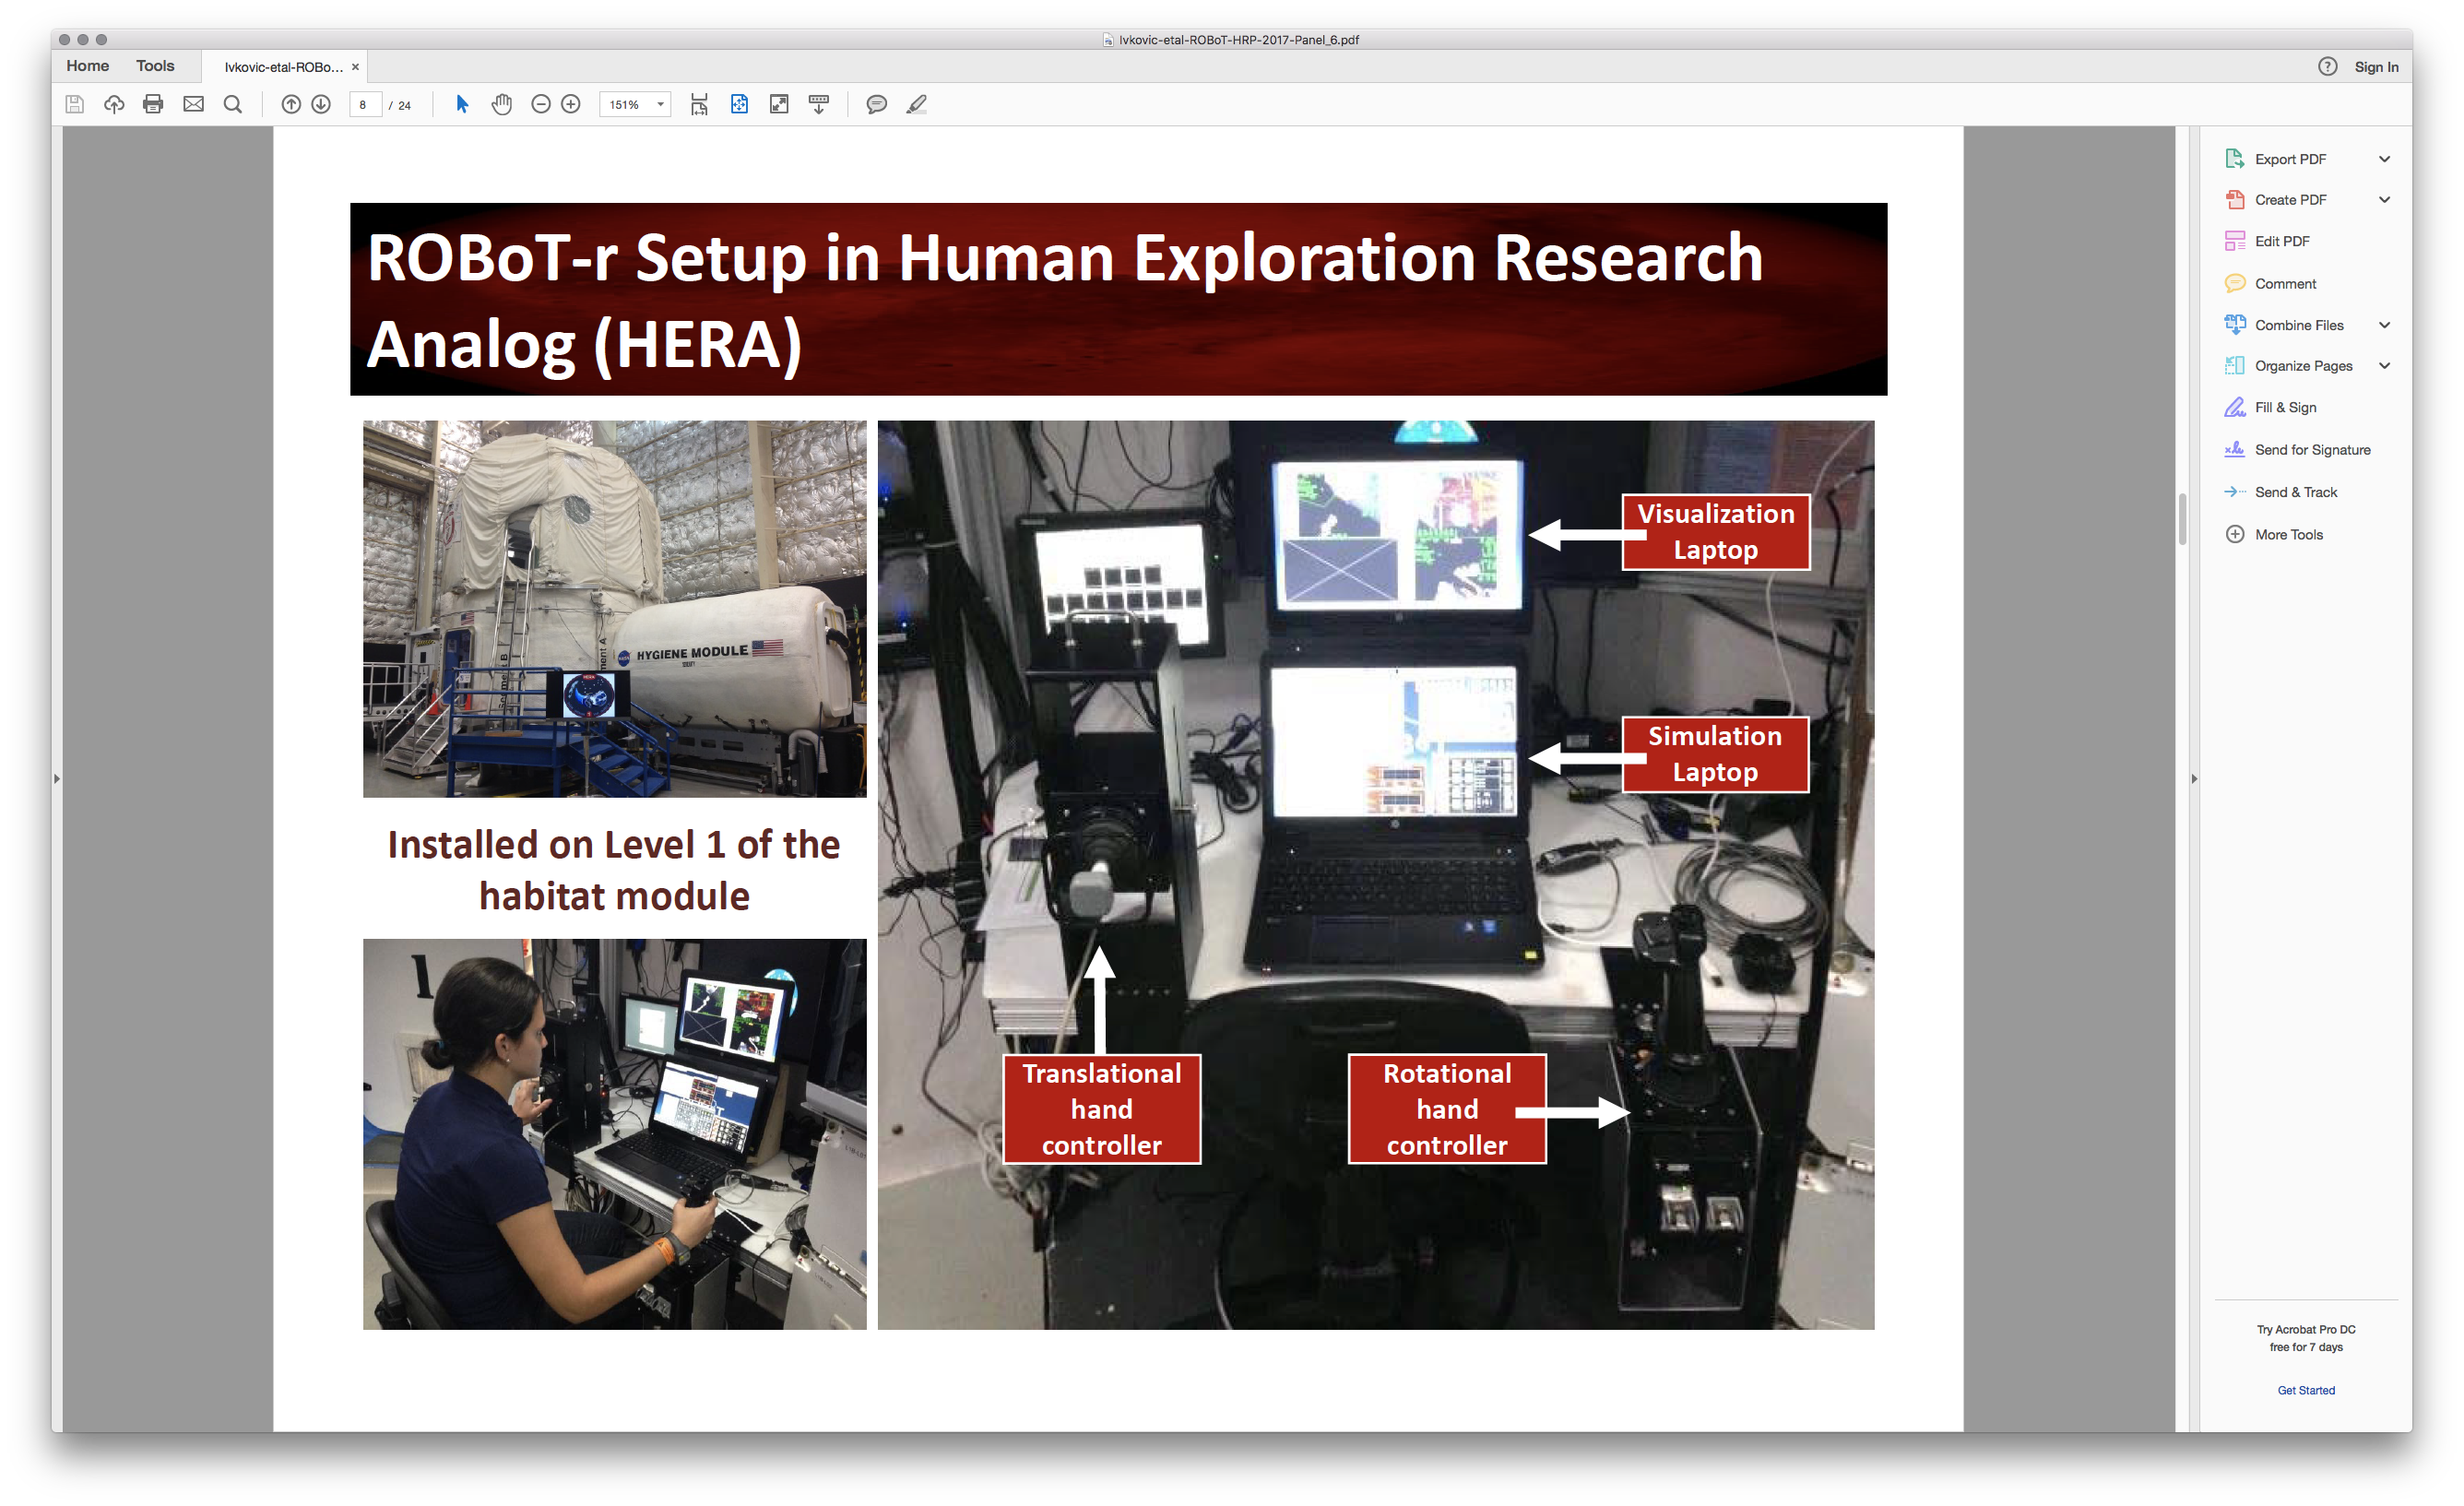
\includegraphics[trim={13cm 5cm 22cm 15.5cm},clip,width=\linewidth]{figures/Screen_Shot_2018-07-26_at_1_43_16_PM.png}
        \caption{The Robotic On-board Trainer (ROBoT) station set up in the NASA HERA Analog, from~\citep{robottalk}.}
        \label{figure:robotinhera}
    \end{center}
\end{figure}

The second Aim of the proposal is addressed by Experiment Two.
Experiment Two will focus on if concurrent bandwidth feedback can decrease the required learning time to peak performance in a simulated robotic arm track and capture task.
We will compare task performance throughout training and workload between two groups: a control group, which receives no feedback, and a treatment group, which receives concurrent bandwidth feedback on one or more sensor readouts.
Subjects in both groups will complete the same task, and it is hypothesized that subjects in the treatment group will perform the task better and require less training time to reach peak performance.
This hypothesis is based on the results of the SAFER experiment, as well as the results of Experiment One.

In this task, subjects will command a robotic arm to track an approaching vehicle and grapple with it.
This is motivated by the primary use of the robot arm on the International Space Station, which grasps visiting vehicles when they arrive at the station and then attaches them to a separate fixed location on the station.
Subjects will be trained on this task and will then repeat the task for one to two hours through a variety of slightly different start and end conditions.

NASA's Robotic On-board Trainer (ROBoT) will be used for this experiment.
ROBoT is a package of simulation software which includes a dynamic model of the robotic arm on the space station and presents the user with multiple camera angle views and the instrument panel required to operate the robotic arm, see Figure~\ref{figure:robotinhera}.
In addition to these displays, ROBoT also includes the two hand controllers required to control the arm.
NASA trainers at Johnson Space Center developed metrics for performance which are included in ROBoT and include the time to capture, the alignment measurements during approach, the amount of wobble in the arm, the number of times the grapple fixture contacted the structure, the overall path efficiency, and the number of capture attempts.
The preceding list presents candidate metrics from which we may observe human performance.

\subsubsection{Hypotheses}
This study will assess the influence of concurrent bandwidth feedback (with vs. without) on performance and workload.
Objective performance data will be measured using time to capture, alignment error metrics, and other metrics available by the ROBoT system.
Subjective workload will be measured using the NASA-TLX at several points throughout the experiment.
It is hypothesized that:
\begin{description}[align=left]
\item [Hypothesis 1] Concurrent bandwidth feedback will improve performance in the track-and-capture task.
\item [Hypothesis 2] Concurrent bandwidth feedback will cause subjects to more quickly reach their peak performance in the track-and-capture task.
\item [Hypothesis 3] Concurrent bandwidth feedback will decrease workload in the track-and-capture task.
\end{description}

\subsubsection{Previous Work}
We have experience using the ROBoT simulation software from participating in a study investigating the effects of sleep loss and circadian misalignment on performance on the ROBoT simulator at NASA Ames~\citep{robotreport}.
In this study, subjects trained during one-hour long sessions each day for five days, then spent a twenty four hour period in the lab while they continued to perform robotic tasks.
We did not find evidence of performance loss during sleep deprivation or circadian misalignment on any of the ROBoT performance metrics.
In fact, participants continued to show improvement over time, which indicated that they had continued to learn the task despite the sleep loss~\citep{robotreport}.
This finding reinforces the need for enhanced learning techniques, as the current training strategy requires a tremendous amount of time to reach peak performance.

% \begin{figure}[tb!]
%     \begin{center}
%         \includegraphics[trim={13cm 5cm 22cm 15.5cm},clip,width=\linewidth]{./../img/Screen Shot 2018-07-26 at 1.43.02 PM.png}
%         \caption{ROBoT visualization laptop, showing four camera views.}
%         % \label{}
%     \end{center}
% \end{figure}

% \begin{figure}[tb!]
%     \begin{center}
%         \includegraphics[trim={13cm 5cm 22cm 15.5cm},clip,width=\linewidth]{./../img/Screen Shot 2018-07-26 at 1.43.05 PM.png}
%         \caption{The camera attached to the end effector of the robotic arm, showing the grapple fixture.}
%         % \label{}
%     \end{center}
% \end{figure}

% \begin{figure}[tb!]
%     \begin{center}
%         \includegraphics[trim={13cm 5cm 22cm 15.5cm},clip,width=\linewidth]{./../img/Screen Shot 2018-07-26 at 1.43.07 PM.png}
%         \caption{Example performance score report shown to the user after each trial.}
%         % \label{}
%     \end{center}
% \end{figure}

% \begin{figure}[tb!]
%     \begin{center}
%         \includegraphics[trim={13cm 5cm 22cm 15.5cm},clip,width=\linewidth]{./../img/Screen Shot 2018-07-26 at 1.43.10 PM.png}
%         \caption{The hand controller inputs and position and angular errors are also logged throughout the trial.}
%         % \label{}
%     \end{center}
% \end{figure}

\subsection{Model Extension}
The third and final Aim of the proposal is addressed by developing a model of the human pilot which includes the effects of concurrent bandwidth feedback.
The proposed Model will extend Professor Hess' structural model of the human pilot to include the effects of concurrent bandwidth feedback.
The Structural Model has been extremely successful in predicting human performance through a variety of system dynamics and can predict how performance changes during a pilot's adaptation to changing dynamics.
Hess has developed adaptive logic for the human pilot in a pursuit task which triggers when the pilot notices that vehicle dynamics have changed~\citep{hess_modeling_2009}.
This logic is based off several criteria, which ``must be predicated upon information available to the human [and] the postadapated pilot models must follow the dictates of the crossover model of the human pilot~\citep{hess_modeling_2009}.''
The primary result of the adaptive logic is to increase the resulting crossover frequency of the pilot, effectively making them more responsive, which could be interpreted as more focused on the task.
Our initial approach to adding concurrent bandwidth feedback into the Structural Model will be based off of Hess' approach to modeling human adaptation in pursuit tasks, which is currently ad-hoc in nature, see Figure~\ref{figure:hesspursuit}.

\begin{figure}[tb]
    \begin{center}
        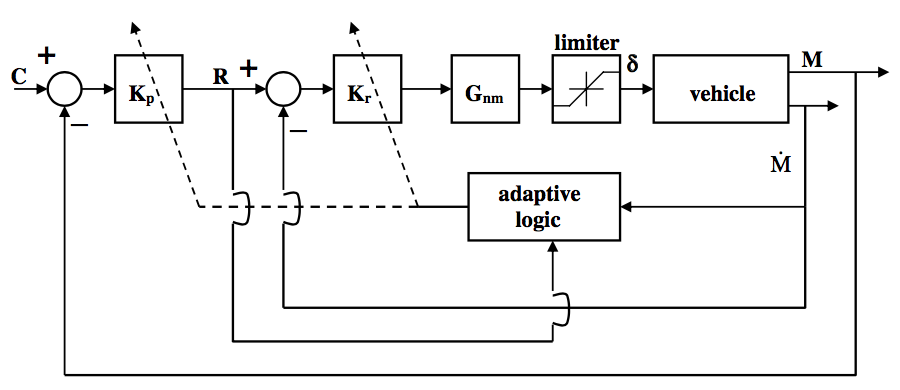
\includegraphics[width=0.8\linewidth]{figures/Screen_Shot_2018-08-09_at_4_15_24_PM.png}
        \caption{Hess' model of the adaptive human pilot, from~\citep{hess_modeling_2009}.}
        \label{figure:hesspursuit}
    \end{center}
\end{figure}

While this model of the adaptive pilot has been successful in predicting changes in performance for a well trained subject, it does not consider how a pilot would behave when they are still in the early stages of training.
Our modified model will include two major changes to Hess' current model:
\begin{itemize}
\item The adaptation logic will be changed to focus on concurrent bandwidth feedback
\item The timescale of the adaptation will be significantly longer
\end{itemize}

We propose to modify the adaptive logic to trigger when the pilot is receiving concurrent bandwidth feedback, rather than when a change in system dynamics occurs.
This will require the addition of a feedback loop onto the Structural Model which triggers when the bandwidth feedback is activated.
This loop will likely be based around the $K_e$ gain, which is currently the primary way of setting the crossover frequency in the Structural Model.
This implies that the subjects in our experiments do their primary learning when they are receiving qualitative feedback that their current level of aggressiveness is not sufficient to complete the task.
While there must be a separate loop that adjusts the crossover frequency as learning progresses over the course of several hours, the change in performance we see when subjects use the concurrent bandwidth feedback happens relatively rapidly, within a few minutes.
This is reflected in the delta of performance between subjects in the different groups of our SAFER experiment, even on the first trial, see Figure~\ref{figure:saferdistance}.
This relates to the second required change, the amount of required adaptation time.
Professor Hess' model requires that pilots adapt within a very short time period, on the order of 5 seconds~\citep{weir_model_1966}.
The results of our experiment with SAFER and the three-axis tracking task also suggest relatively short adaptation times, though they are on the order of a few minutes, again see Figure~\ref{figure:saferdistance}.

While it should be noted that this work is in preliminary stages and not scheduled to begin until the Fall Quarter, some early work has been started in preparation for the qualifying examination.
An effort has been made to begin to replicate some of Hess' results.
Working with Professor Hess, we have been able to replicate some of the existing adaptation logic for a two-axis tracking task, and begun exploratory research into modifying the model.


%!TEX root = ../main.tex
% \documentclass[float=false, crop=false]{standalone}
% \usepackage[subpreambles=true]{standalone}
% \begin{document}

\section{Timeline and Risks}
% \begin{figure}[h!]
%     \begin{center}
%         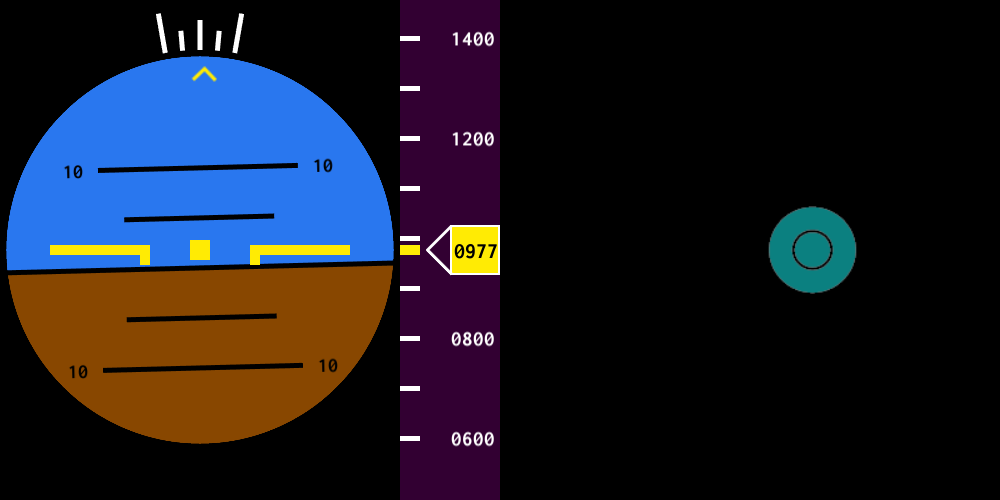
\includegraphics[width=\linewidth]{./../img/image1.png}
%         \caption{The proposed timeline for this research.}
%         \label{timeline}
%     \end{center}
% \end{figure}

The proposed timeline for the remainder of this research is available in Figure%~\ref{timeline}.
This timeline shows the past few months spent accomplishing the first aim and outlines our estimated timeline to complete the remaining aims, with an estimated graduation date of Summer Quarter 2020.
While not present on the timeline, we also plan to write and submit several conference papers and journal articles throughout the completion of this research.

A conference paper, ``Evaluating Augmented Reality in a Three-Axis Manual Tracking Task'', J. Karasinski and S. Robinson has recently been submitted for consideration at AIAA SciTech 2018.
A draft journal article on the SAFER experiment is being prepared for submission in the journal of Human Factors.
We expect to publish an additional conference paper to an AIAA or IEEE conference and journal article for the results of the robotic arm experiment, likely in Human Factors.
If we are successful in creating a model which closely follows human behavior, we would also publish this as a journal article, likely in the Journal of Guidance, Control, and Dynamics.

% This timeline was created under the assumption that everything will go according to plan, which is almost certainly not the case.
This schedule is flexible to changes in plans, and was designed with the full awareness that we may face setbacks.
There are a number of places where we may suffer delays or other issues:
\begin{itemize}
\item% 
% It is difficult to predict how long it will take to recruit subjects and run them through an experiment.
While the author has experience subject testing over one hundred subjects over three hundred hours of experiment time, it is difficult to predict how long subject testing will take to complete.
Under the assumption that we will run approximately twenty to thirty subjects in the robotic arm experiment, and that the experiment will last for approximately two to three hours per subject, we have budgeted one quarter to recruit subjects and run them through the experiment.
This could, however, easily stretch to two quarters, depending on subject availability and success rates.
\item NASA Ames has agreed to allow the Human/Robotics/Vehicle Integration and Robotics Lab to use the ROBoT simulator for this proposed experiment at UC Davis.
If, for whatever reason, we are unable to use ROBoT, we could either run the experiment at Ames or attempt to build our own robotic arm simulation.
\item While we believe we have sufficient evidence that our feedback techniques will improve performance, it is also possible that we will not see significant effects in the robotic arm task.
If this is the case we will need to further investigate how this task is different from our previous successes.
This would allow us, for instance, to make begin to make recommendations for which types of tasks can and cannot benefit from this feedback.
\item It is possible that we may be unable to create a model which incorporates feedback and that accurately mirrors the effects we have seen in our experiments. This may require us to investigate other types of performance models or to create a novel technique.
\end{itemize}

\chapter{Augmented Reality Tracking Task}
\label{chap:3dtracking}

Portions of this chapter were originally published in the conference proceedings for AIAA Modeling and Simulation Technologies 2019 \citep{karasinski_evaluating_2019}.

% \begin{abstract}
% Recent advances in computing hardware have enabled a new generation of mobile augmented reality devices which have the potential to improve human performance and reduce workload in a variety of tasks.
% The aim of this study was to investigate the effect of several factors on human performance and workload in a three-axis manual tracking task.
% Twenty four (24) engineering students at the University of California, Davis were randomly placed into a one of two device groups ($n=12$ per group): a 2D or 3D display.
% Subjects in both groups evaluated three different displays in a random order: a baseline display, a concurrent bandwidth feedback display, and an rotated display.
% Subjects' objective performance was evaluated using the root-mean-square error (RMSE) of the depth ($z$) axis.
% Objective workload was measured by the response time to a two-choice task, and subjective workload was evaluated using the NASA Task Load Index (NASA-TLX).
% Results of ANOVA analysis on the $z$ axis RMSE showed significant effects for design ($F(2, 36)=84.92, p<.001$), device ($F(1, 18)=7.22, p<0.015$), and start design ($F(2, 18)=4.81, p<0.021$).
% The ANOVA also showed a significant interaction effect between design and starting design ($F(4, 36)=8.55, p<0.0001$), and a three way interaction between design, device, and starting design ($F(4, 36)=5.57, p<0.002$).
% In general, there were no significant effects found for workload measurements.
% Both concurrent bandwidth feedback and a rotated display resulted in superior performance when compared to a baseline display.
% Providing a 3D display did not, in general, improve performance.
% Subjects in the 3D display group and that had early exposure to the concurrent bandwidth feedback, however, were able to use the feedback to achieve superior performance.
% \end{abstract}

\section{Introduction}
\subsection{Overview}
Recent advances in computing hardware have enabled a new generation of mobile augmented reality devices which have the potential to improve human performance and reduce workload in a variety of tasks.
The aim of this study was to investigate the effect of several factors on human performance and workload in a three-axis manual tracking task.
The Microsoft HoloLens is a head-mounted, mobile augmented reality device which provides a stereoscopic 3D view to the user which is not available with traditional 2D displays.
To evaluate whether this new display technology could improve user performance in a tracking task, we designed an experiment that investigated if the depth cueing delivered by stereoscopic display could provide improved performance and decreased workload.
We were also interested to see if a 2D display could gain the benefits of a depth cue by rotating the axis of the task such that the depth cue was more readily available.
Research has also shown that presenting three-dimensional information on a two-dimensional screen is not a simple task, and that the projection of the 3D information onto the 2D screen can cause large changes in the performance of the user~\citep{kim_quantitative_1987}.
In addition to these cues, we also investigated the effects of concurrent bandwidth feedback on task performance and workload as an alternate technique to improving performance.
Concurrent bandwidth feedback alerts the operator when their real-time performance has drifted outside an acceptable, predefined window of performance.
The use of this type of feedback has been shown to improve performance in a wide variety of motor control tasks~\citep{salmoni_knowledge_1984,sigrist_augmented_2013,karasinski_real-time_2017}.

\subsection{Literature Review}
\subsubsection{Augmented Feedback}
The concept of feedback was popularized when closed-loop control systems were first developed and has since been defined many times~\citep{Wierner1948}.
In the context of this work, a convenient definition of feedback comes from Ramaprasad, ``[f]eedback is information about the gap between the actual level and the reference level of a system parameter which is used to alter the gap in some way~\citep{ramaprasad_definition_1983}.''
The aforementioned ``gap'' is the error and can be conveyed to the operator of a system in a variety of ways.
Feedback can be broadly classified into two types: intrinsic, feedback which is generated from within the context of the action itself, and extrinsic, feedback which is given from an external source~\citep{laurillard_rethinking_2002}.

Extrinsic feedback, which is also known as augmented feedback, has been extensively studied in the field motor learning~\citep{sigrist_augmented_2013}.
In their 2013 review, Sigrist et al. write ``[i]t is generally accepted that augmented feedback, provided by a human expert or a technical display, effectively enhances motor learning~\citep{sigrist_augmented_2013}.''
There are a variety of different forms of augmented feedback, that can be further classified by how, when, and by what form the feedback is provided.
Concurrent, or real-time, feedback is displayed to the operator while the task is being executed, in contrast to terminal feedback, which is displayed after the task is complete.
Bandwidth feedback is displayed to the operator when some parameter is inside (on-track feedback) or outside (off-track feedback) of an acceptable, predefined tolerance limit.

Experimentation with bandwidth feedback traces its origins to Thorndike's 1927 line-drawing experiment~\citep{thorndike_law_1927}.
In his experiment, subjects were seated and blindfolded at a table, then asked to draw lines of 3, 4, 5, or 6 inches.
The experiment was divided into two groups of subjects, one group of subjects received no verbal feedback, while the other group was told ``right'' if they were within an 1/8th of an inch of the desired length for the 3 inch line, or 1/4 of an inch for the other three line lengths, and ``wrong'' if they were outside this bandwidth.
Subjects that received the verbal bandwidth feedback improved from an initial median ``right'' percentage of 13\% to 54\% after several training sessions.
The feedback was then removed after these training trials, during which time subjects dropped to a median percentage of 26\%.
This is consistent with the guidance hypothesis (which was not formalized for another fifty years after this experiment was concluded), which states that consistent feedback during the acquisition phase of learning leads to a dependency on the feedback~\citep{salmoni_knowledge_1984}.
Subjects became dependent on the verbal feedback (extrinsic feedback) rather than their visual or proprioceptive sense (intrinsic feedback) to such an extent that they could no longer perform with the verbal feedback removed.

Payne and Hauty performed one of the first concurrent bandwidth feedback studies in 1955~\citep{payne_effect_1955}.
In their study, subjects completed a multidimensional pursuit test, which required them to scan four simulated aircraft instruments and counter their drift by adjusting simulated aircraft controls.
Subjects were placed into one of three feedback groups: a control level, where no feedback was provided, a second level, which included a single peripheral visual signal when a deviation in one of the displays occurred, but did not specify which instrument, and a third level, which provided individual indicators for each of the four instruments, and noted the locus of the deviation.
They found a very significant effect between the different feedback groups, with the control group performing the worst, the second level performing better, and the third level performing better still.
Subjects completed the test every hour for a four hour period.
Performance dropped across all three groups as time elapsed and subjects fatigued, but the performance of the subjects in level three was superior at the end of this period compared to the subjects in the control group at the beginning of the experiment.
They concluded by stating that ``the increment is a positive function of the specificity of the information supplied, it can be ascribed largely to the directive properties of the cues, i.e., the cues impose a more efficient temporal and spatial organization upon [the subject's] scanning behavior~\citep{payne_effect_1955}.''

Gordon and Gottlieb performed a rotary pursuit study investigating the effects on on-track and off-track concurrent bandwidth feedback in 1967~\citep{gordon_effect_1967}.
Subjects in their study were placed into one of three groups: a control, on-track feedback, and off-track feedback.
The subjects in the bandwidth feedback groups had to track a 0.75 inch by 0.75 inch target with 0.187 inch rigid stylus tip.
For subjects in the on-track feedback group, a light bulb was illuminated when they were on target, and the light bulb was illuminated for subjects in the off-track group when they were not on the target.
While both the on-track and off-track groups performed better than the control group, the off-target group performance was slightly superior.
This finding was consistent with the results Williams and Briggs found in a similar task~\citep{williams_-target_1962}.
Additionally, subjects in the feedback groups completed several trials at the end of the experiment without feedback and did not experience the loss of performance which is often seen due to the guidance hypothesis.
This indicates that subjects were able to use the feedback to better learn the task and were not completely dependent on the feedback.
Subjects used their own intrinsic feedback to learn the task, and were able to take advantage of the concurrent bandwidth feedback to better learn and perform the task without becoming dependent on the external feedback.

Recent work in the field has taken advantage of modern computing and visualization technology to produce higher fidelity simulations.
In 2011, de Groot et al. investigated the effects of concurrent bandwidth feedback on learning a lane-keeping task in a driving simulator~\citep{de_groot_effect_2011}.
Similar to Gordon and Gottlieb, they investigated the effects of on-track and off-track feedback compared to a control group~\citep{gordon_effect_1967}.
Instead of using a visual indicator, however, de Groot et al. used haptic feedback in the form of a vibrating chair for their feedback groups~\citep{de_groot_effect_2011}.
They found that on-target and off-target groups had better lane-keeping performance than the control group, and that, similar to Gordon and Gottlieb and Williams and Brigg, the off-target group performed best~\citep{gordon_effect_1967,williams_-target_1962}.
Retention trials, however, showed that a majority of this performance improvement was lost during when the feedback was removed, which was in accordance with the guidance hypothesis.
The off-target group, though, did still retain some minor performance improvement, which the authors partially attribute to the onset advantage~\citep{fischer_differential_2008}.
The onset advantage ``suggests that the sudden onset of a stimulus is a more powerful perceptual event than a stimulus offset, facilitating low-level perceptual processing and resulting in faster reaction times~\citep{de_groot_effect_2011}.''
This effect could explain a repeated finding that off-track feedback is superior to on-track feedback, even if the effect is, in general, small.
de Groot et al. also measured response time to a secondary task as an estimate of workload, but found no differences across groups.

\subsubsection{SAFER Experiment}
\begin{figure}[b!]
    \begin{center}
        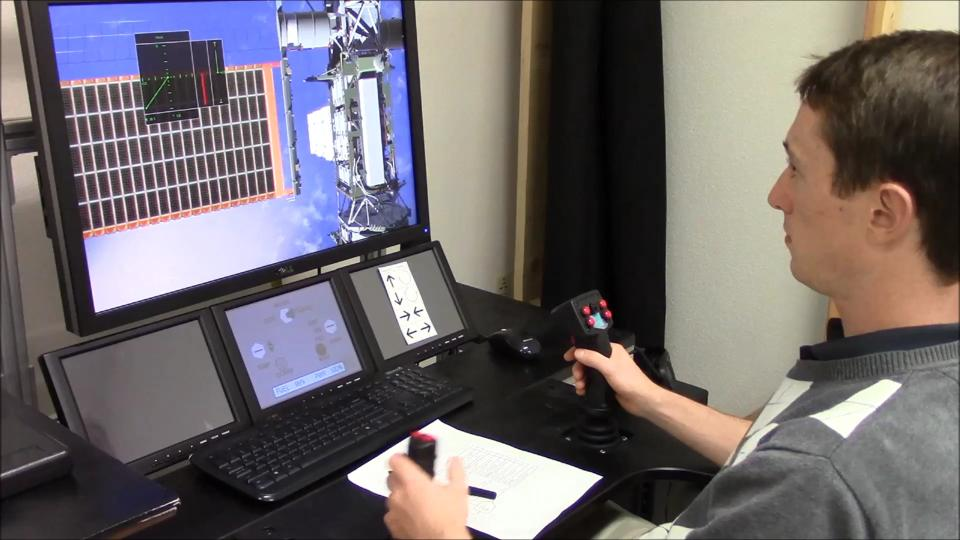
\includegraphics[width=0.8\linewidth]{figures/AR/SAFER_DangerChris.jpg}
        \caption[Simplified Aid for EVA Rescue (SAFER) experiment subject seated in the fixed-base simulator]{A subject from the Simplified Aid for EVA Rescue (SAFER) experiment seated in the fixed-base simulator~\citep{karasinski_real-time_2016}.}
        \label{figure:safersim}
    \end{center}
\end{figure}

Our recent work includes investigations into concurrent bandwidth feedback in a four degree of freedom Simplified Aid for EVA Rescue (SAFER) task~\citep{karasinski_real-time_2016, karasinski_real-time_2017, karasinski_development_2016}.
SAFER is a small propulsive jet pack worn during spacewalks for self-rescue~\citep{Vassigh1998}.
Subjects were tasked with flying a SAFER simulation to perform an inspection of the International Space Station's (ISS) solar arrays.
Subjects were initially placed 40 feet away from the solar array and were asked to close to 30 feet and hold this distance for the remainder of the task.
They could gauge their distance from the solar array using the indicator on the guidance display and the out-the-window display.
Subjects were then asked to inspect four waypoints on the solar array, and were given a guidance display for navigation to the waypoints.
Two vertically arranged displays in the simulator were available to complete the task (see Fig.~\ref{figure:safersim}).
The primary display contained an out-the-window view of the solar array and, depending on which group the subject was in, one of the guidance displays.
The secondary display located directly below the primary display portrayed information about the subject's current mode, remaining fuel, and a ``comm light''.

\begin{figure}[tb!]
    \begin{center}
        \begin{subfigure}{0.49\textwidth}
            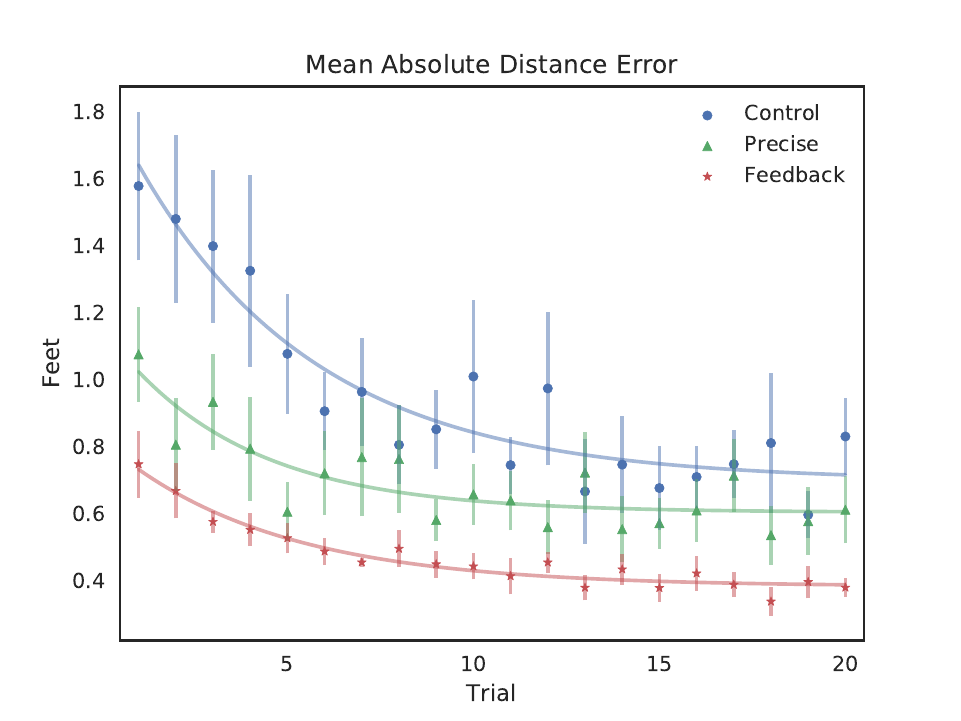
\includegraphics[width=\linewidth]{figures/AR/Group_absDistErr_clean_fit_30.png}
            \caption[Mean absolute distance error]{Mean absolute distance error, by group.}
            \label{figure:saferdistance}
        \end{subfigure}\hfill
        \begin{subfigure}{0.49\textwidth}
            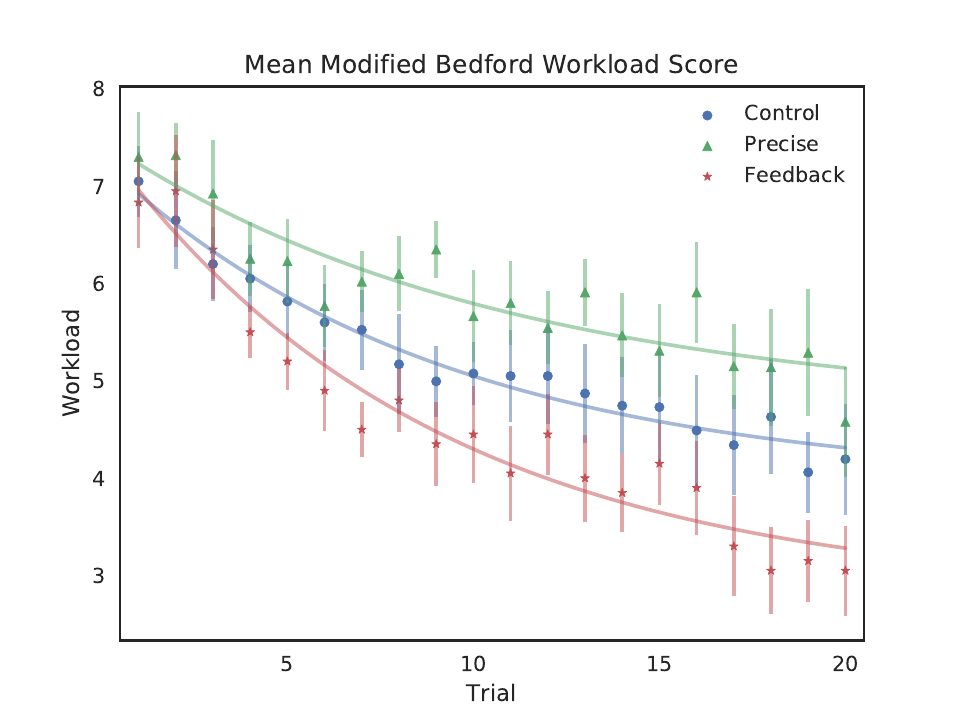
\includegraphics[width=\linewidth]{figures/AR/Group_Workload_fit_30.png}
            \caption[Mean subjective workload rating]{Mean subjective workload rating, by group.}
            \label{figure:saferworkload}
        \end{subfigure}
        \caption[Performance and workload benefits from feedback]{Subjects with concurrent bandwidth feedback (CBF) performed the best (a) and reported the lowest workload (b). Errors are the standard error of the mean~\citep{karasinski_real-time_2016}.}
    \end{center}
\end{figure}

In our experiment, subjects were placed into one of three groups: a control, a high precision augmented feedback group, and a concurrent bandwidth feedback (CBF) group.
Subjects in the high precision group were given an extra significant figure in their guidance display and an analog display which was scaled twice as large (but had half the maximum value) of their flight parameters.
Subjects in the CBF group had two display elements which would change from a green to a red color when the subject's performance was outside a predefined range.
Performance was measured as mean absolute distance error (MAE) and results across trials are shown in Fig.~\ref{figure:saferdistance}.
Both treatment groups performed better than the control group, with the CBF group performing the best and having the least error.
The effects that the treatments had on workload was very different than performance, however.
Subjects in the high precision group reported significantly more workload than the control group, while subjects in the CBF group reported significantly less workload than the control group (see Fig.~\ref{figure:saferworkload}).
The concurrent bandwidth feedback also had the added benefit of significantly reducing the amount of time required to train the subjects to their maximum skill level.
Subjects with the CBF performed better on their first trial than subjects in the control group did on their last, which was after approximately two hours on the task.

\subsubsection{Stereoscopic Displays}
Stereoscopic displays are systems ``in which two slightly different views of a scene are provided to a viewer, one image for each eye... allow[ing] the viewer's binocular visual system to extract depth information in a scene using this disparate information''~\citep{mcintire_stereoscopic_2014}.
Without the aid of the binocular depth cue presented by stereoscopic displays, viewers are instead entirely reliant on monocular clues such relative sizing, occlusion, and motion.
One of the primary motivation for stereoscopic displays is that ``[t]he visual scene of a 3D world is a more `natural,' `ecological,' or `compatible' representation than that provided by 2D displays''~\citep{wickens_three-dimensional_1990}.
As a result of this motivation, the effects of stereoscopic displays on human performance have been extensively studied in the literature.
Several authors have attempted to classify which types of tasks may stand to benefit~\citep{mcintire_stereoscopic_2014, wickens_three-dimensional_1990, wickens_three-dimensional_1989, naikar_perspective_1998, dixon_human_2009}.
A recent review of 184 papers, for example, suggests that 60\% of studies showed some benefit of 3D stereo displays, 15\% of tasks showed unclear or mixed benefits, and 25\% of studies showed no clear benefits~\citep{mcintire_stereoscopic_2014}.
In their review, tasks involving finding/identifying/classifying objects and tasks involving real/virtual spatial manipulations of objects benefited the most, while learning/training/planning tasks were the least likely to show a benefit.

Kim et al. also performed a quantitative evaluation of perspective and stereoscopic displays in a three-axis manual tracking task~\citep{kim_quantitative_1987}.
They investigated the differences between perspective and stereoscopic displays, the elevation angle, azimuth angle, and the effects of two visual enhancements: a grid and a reference line.
They found very strong relationships between elevation and azimuth angles and tracking performance, with the best performance occurring at an elevation angle of 45 degrees and an azimuth angle of 0 degrees.
Tracking performance decreased rapidly as the azimuth angle varied, and decreased less rapidly as the elevation angle varied.
In general, they found that the stereoscopic display allowed for better tracking performance, though the inclusion of the reference line visual enhancement greatly decreased the benefit over the perspective display.
Using only two subjects, they provided some insight into intrasubject and intersubject variability.
In several instances, intrasubject variability showed 50\% changes within the same experimental condition, while intersubject variability also appeared quite large in some conditions.
Kim et al. repeated the evaluation of these parameters on a telerobotics pick-and-place study~\citep{kim_visual_1987}.
They found similar results in this second study, suggesting that their results could be generalized and that three-axis tracking performance can be correlated with pick-and-place completion time.

Smallman at al. similarly investigated the effect of visual enhancements and 2D vs 3D displays for the development of a naval air warfare console~\citep{smallman_track_2000}.
Participants viewed naval and aircraft tracks in either a conventional 2D top-down display or a 3D display, and then attempted to reconstruct track positions.
They investigated the effectiveness of drop-lines and drop-shadows, and found that they significantly improved subjects ability to localize aircraft compared to when the enhancements were not present.
Furthermore, in the absence of either visual enhancement, subjects performed better with the 2D display than the 3D display.
Similar to Kim et al., they ultimately recommended that 3D stereoscopic displays include the use of a reference or drop-line for optimal performance.

\subsubsection{Workload Measurement}
Improving performance, through some kind of feedback or other technique, often comes at the cost of increased workload, which can lead to a loss of the ability to maintain performance.
Workload was defined by Hart and Staveland as ``the perceived relationship between the amount of mental processing capability or resources and the amount required by the task''~\citep{hart_development_1988}.
Having a low workload indicates that it would be easy to complete additional tasks, while having a high workload suggests that it would be difficult.

The NASA Task Load Index (NASA-TLX) is one of the most well known and commonly used subjective workload measures.
The NASA-TLX has been in use for thirty years, and has been used and validated over a large variety of tasks~\citep{hart_nasa-task_2006}.
The NASA-TLX is a multidimensional rating scale which uses the magnitude and ranking of six subscales to produce an overall estimate of subjective workload~\citep{hart_development_1988}.
The six subscales are: Mental Demand, Physical Demand, Temporal Demand, Performance, Effort, and Frustration.
Each of these scales is rated on a 0 (Very Low) to 100 (Very High) scale, with the exception of Performance, which is rated from 0 (Perfect) to 100 (Failure).
After marking a value for each of these subscales, subjects then make fifteen pairwise weightings, allowing them to rate each pair of subscales based on its perceived contribution to their overall workload.
A final, overall workload score is computed by multiplying each subscale's score by the number of times it was chosen in the pairwise weightings, adding these values, and dividing by fifteen.
As certain subscales may be more or less important than others, depending on the task being evaluated, some researchers can drop subscales or simply not compute the overall score.

In addition to subjective measures of workload, there are a variety of techniques which aim to estimate objective workload.
One of the most common objective measurement techniques is the secondary task, which requires subjects to complete the primary task, then use any spare workload to respond to an additional task~\citep{gawron_human_2008}.
Secondary tasks can provide a measure more sensitive to differences in workload and performance than a single task alone and allow for a common measure between experimental conditions~\citep{slocum1971meaningful}.
Care must be taken, however, to ensure that the secondary task does not intrude upon primary task performance~\citep{williges_behavioral_1979}.
In our previous studies, we have used a multiple choice reaction time task as an objective workload measurement.
In this secondary task, subjects are presented with several different stimuli, each of which requires a different response~\citep{lysaght_operator_1989}.
A subject's objective workload can then be inferred by either the percentage of secondary tasks which were correctly responded to within a given time, the number of secondary tasks which were correctly responded to in a trial, or both.
We have previously found this type of task to be correlated with subjective workload scales in the aforementioned SAFER task~\citep{karasinski_real-time_2017}.

\subsubsection{Summary}
Concurrent bandwidth feedback has been used in a large variety of motor control tasks, and has generally been found to improve performance.
Until recently, however, only simple tasks such as physical movements or basic pursuit tasks have been investigated.
More recent works, including the lane-keeping task by de Groot et al., and our previous work with the SAFER task, have indicated that concurrent bandwidth feedback can also be quite effective for complex tasks.
The decrease in required learning time, improved performance, and decreased workload seen in the SAFER task show that concurrent bandwidth feedback may prove to be most useful very early in training when subjects are first exposed to complex, highly dynamic tasks.
While visual concurrent bandwidth feedback has been used in a variety of tasks, no researchers have investigated its effects on a three-axis tracking task.

Despite extensive previous research, to the authors' knowledge there exists no study in the literature addressing human performance or workload changes in manual tracking tasks between traditional computer monitors and mobile, augmented reality headsets.
If operator performance while using augmented reality displays is improved--or at the very least, not degraded--then these devices could prove especially valuable in scenarios where it is impractical or otherwise difficult to provide a traditional computer interface.
There are a variety of robotics tasks, such as pick-and-place tasks, for which performance may be improved by allowing an operator the mobility to move and view the scene from whatever position is convenient at a given time.
Traditional robotics stations require the operator to remain in a single position, and typically only allow for several camera angles.
Mobile augmented reality displays allow the operator to take advantage of their ability to move through the environment, without needing to manage external cameras.

\section{Materials and Method}
\begin{figure}[b!]
    \begin{center}
        % Thanks
        % https://tex.stackexchange.com/questions/67573/tikz-shift-and-rotate-in-3d

        \newcommand{\rotateRPY}[3]% roll, pitch, yaw
        {   \pgfmathsetmacro{\rollangle}{#1}
            \pgfmathsetmacro{\pitchangle}{#2}
            \pgfmathsetmacro{\yawangle}{#3}

            % to what vector is the x unit vector transformed, and which 2D vector is this?
            \pgfmathsetmacro{\newxx}{cos(\yawangle)*cos(\pitchangle)}
            \pgfmathsetmacro{\newxy}{sin(\yawangle)*cos(\pitchangle)}
            \pgfmathsetmacro{\newxz}{-sin(\pitchangle)}
            \path (\newxx,\newxy,\newxz);
            \pgfgetlastxy{\nxx}{\nxy};

            % to what vector is the y unit vector transformed, and which 2D vector is this?
            \pgfmathsetmacro{\newyx}{cos(\yawangle)*sin(\pitchangle)*sin(\rollangle)-sin(\yawangle)*cos(\rollangle)}
            \pgfmathsetmacro{\newyy}{sin(\yawangle)*sin(\pitchangle)*sin(\rollangle)+ cos(\yawangle)*cos(\rollangle)}
            \pgfmathsetmacro{\newyz}{cos(\pitchangle)*sin(\rollangle)}
            \path (\newyx,\newyy,\newyz);
            \pgfgetlastxy{\nyx}{\nyy};

            % to what vector is the z unit vector transformed, and which 2D vector is this?
            \pgfmathsetmacro{\newzx}{cos(\yawangle)*sin(\pitchangle)*cos(\rollangle)+ sin(\yawangle)*sin(\rollangle)}
            \pgfmathsetmacro{\newzy}{sin(\yawangle)*sin(\pitchangle)*cos(\rollangle)-cos(\yawangle)*sin(\rollangle)}
            \pgfmathsetmacro{\newzz}{cos(\pitchangle)*cos(\rollangle)}
            \path (\newzx,\newzy,\newzz);
            \pgfgetlastxy{\nzx}{\nzy};
        }

        \tikzset{RPY/.style={x={(\nxx,\nxy)},y={(\nyx,\nyy)},z={(\nzx,\nzy)}}}

        \begin{tikzpicture}
            \draw[-] node at (3.5,0,0) {$x$} (-3,0,0) -- (3,0,0);
            \draw[-] node at (0,3.5/2,0) {$y$, {\color{red} $y\textprime$}} (0,-3/2,0) -- (0,3/2,0);
            \draw[-] node at (0,0,3.5) {$z$} (0,0,-3) -- (0,0,3);

            \rotateRPY{0}{-30}{0}
            \begin{scope}[draw=red, text=red,fill=red,densely dashed,RPY]
                \draw[-] node at (3.5,0,0) {$x\textprime$} (-3,0,0) -- (3,0,0);
                %\draw[-] node at (0,3.5,0) {} (0,0,0) -- (0,3,0);
                \draw[-] node at (0,0,3.5) {$z\textprime$} (0,0,-3) -- (0,0,3);
            \end{scope}
            \draw [->] (0:1.5) arc (0:-15:1.5);
            \draw[-] node at (1.7,-.2,0) {$\theta$};
        \end{tikzpicture}

        \caption[Perspective display of the coordinate frame for the tracking tasks]{Perspective display of the coordinate frame for the tracking tasks, with the $x$, $y$, and $z$ axes labeled. After rotating by $\theta$ around the y axis, the resulting reference frame of $x\textprime y\textprime z\textprime$ is also labeled.}
        \label{designdiagram}
    \end{center}
\end{figure}

In our experiment, subjects were responsible for simultaneously completing three primary tracking tasks and a two-choice secondary task.
Each axis of the tracking task was disturbed by a sum-of-sines, resulting in a random appearing signal that was difficult for the subjects to predict.
The two-choice task appeared on a screen next to the tracking task, and asked subjects to respond to either a ``LEFT'' or ``RIGHT'' command by pressing a button.
Subjects controlled the three-axes and responded to the two-choice task by using a Microsoft Xbox controller.
The subjects used the left joystick on the controller to control the $x$ and $y$ axes tracking tasks.
Subjects moved this joystick left and right to control the $x$ axis, and up and down to control the $y$ axis.
The subjects used the right joystick on the controller to control the $z$ axis.
Subjects moved this joystick up and down to control the $z$ axis.
See Fig.~\ref{designdiagram} for a visualization of the coordinate frame of the primary tracking task.
Subjects used the left and right triggers on the controller to respond to the two-choice task, using the left trigger to indicate ``LEFT'' on the two-choice task, and the right trigger to indicate ``RIGHT'' on the two-choice task.

\subsection{Hypotheses}
This study assessed the influence of display type (perspective vs. stereoscopic), relative display attitude (zero degrees vs. thirty degrees), and concurrent bandwidth feedback (with vs. without) on performance and workload.
Objective performance was measured using the root-mean-square error (RMSE) of the depth ($z$) axis.
Objective workload was measured using the response time to the secondary task, and subjective workload was measured using the NASA-TLX.
It was hypothesized that:
\begin{description}[align=left]
    \item [Hypothesis 1] Concurrent bandwidth feedback will improve performance in the depth ($z$) axis for both display types, and will decrease workload.
    \item [Hypothesis 2] Stereoscopic augmented reality displays improve performance in the depth ($z$) axis, but do not affect workload.
    \item [Hypothesis 3] Rotating the display improves performance in the depth ($z$) axis for both display types, and will decrease workload.
\end{description}

\subsection{Procedure}
A total of 24 subjects (19 males, 5 females) were recruited in accordance with the University of California, Davis Internal Review Board (IRB), and subjects were not compensated.
There were 12 subjects in the 2D group, and 12 subjects in the 3D group.
Subjects were students in the University of California, Davis, College of Engineering.
All participating subjects had normal vision (no colorblindness, eyesight correctable to 20/20 vision) and full motor control of their hands.

\begin{figure}[t!]
    \begin{center}
        \begin{subfigure}{0.49\textwidth}
            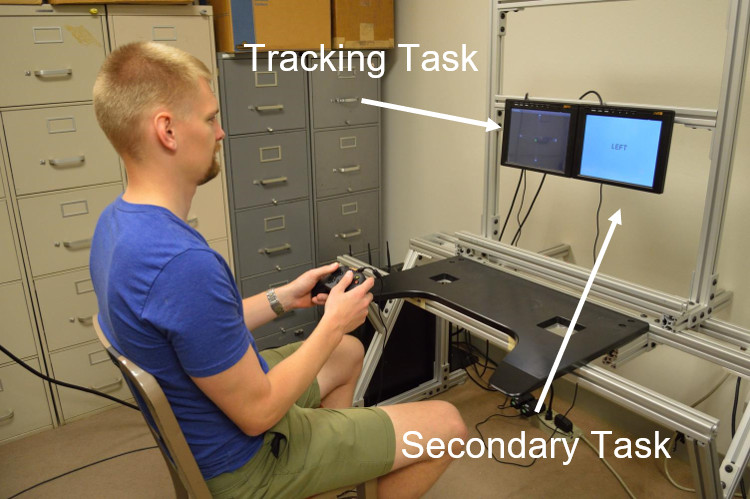
\includegraphics[width=\linewidth]{figures/AR/DSC_0801.JPG}
            \caption[2D Group]{2D Group.}
        \end{subfigure}\hfill
        \begin{subfigure}{0.49\textwidth}
            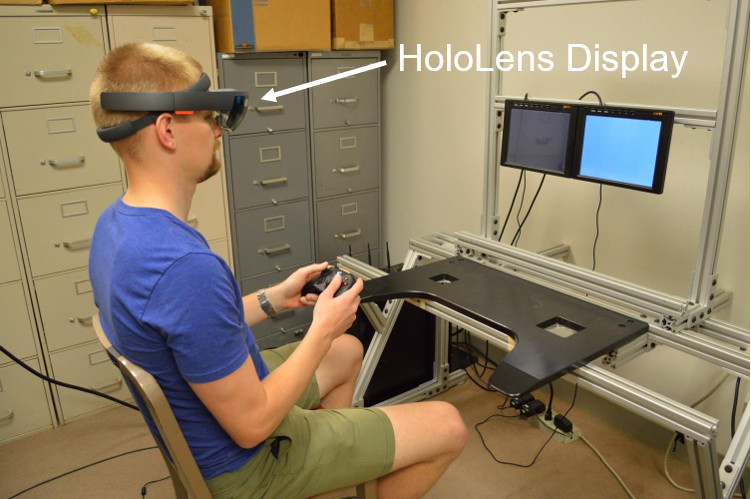
\includegraphics[width=\linewidth]{figures/AR/DSC_0803.JPG}
            \caption[3D Group]{3D Group.}
        \end{subfigure}
        \caption[The fixed-based simulator used by both groups]{The fixed-based simulator used by both groups.}%
        \label{fig:simulator}%
    \end{center}
\end{figure}

\begin{figure}[t!]
    \begin{center}
        \begin{subfigure}{0.32\textwidth}
            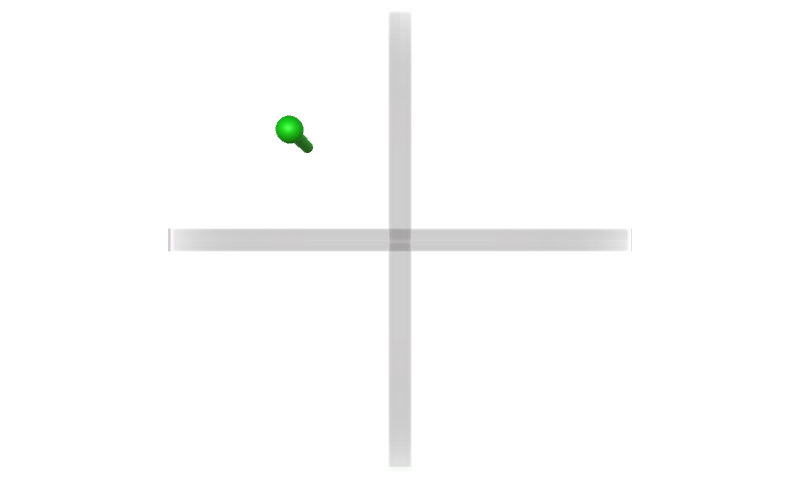
\includegraphics[trim={5cm 0 5cm 0},clip,width=\linewidth]{figures/AR/Baseline.png}
            \caption[Baseline]{Baseline.}
            \label{fig:designs_baseline}
        \end{subfigure}\hfill
        \begin{subfigure}{0.32\textwidth}
            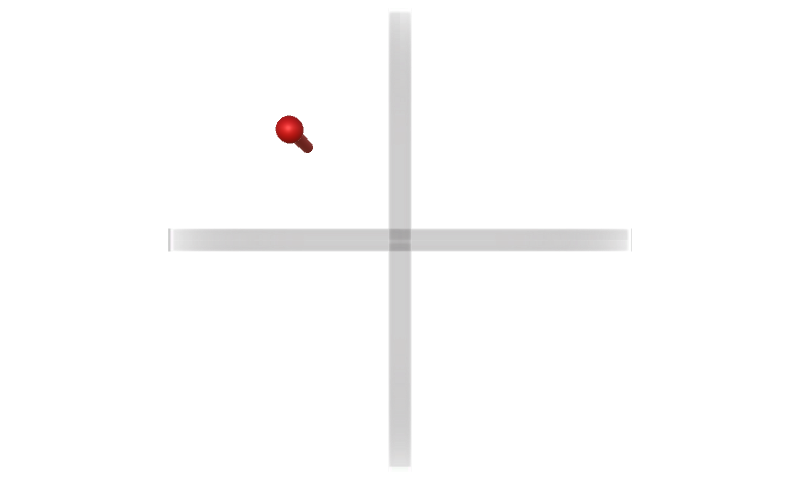
\includegraphics[trim={5cm 0 5cm 0},clip,width=\linewidth]{figures/AR/Color.png}
            \caption[Color Feedback]{Color Feedback.}
            \label{fig:designs_feedback}
        \end{subfigure}\hfill
        \begin{subfigure}{0.32\textwidth}
            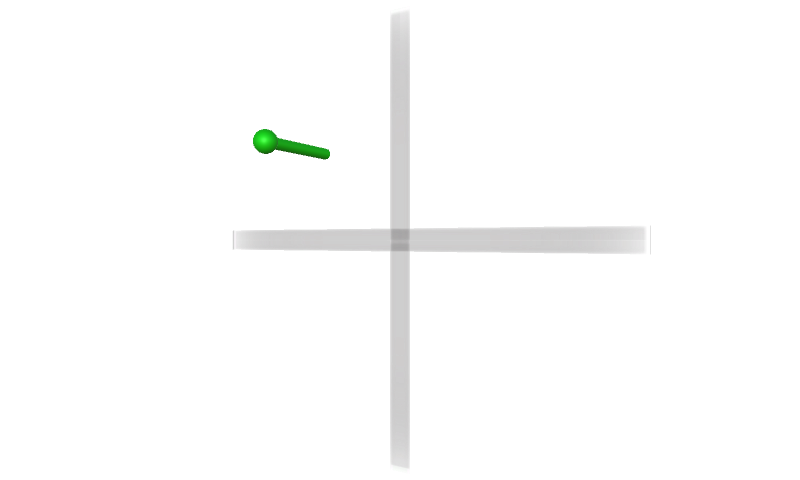
\includegraphics[trim={5cm 0 5cm 0},clip,width=\linewidth]{figures/AR/Angled.png}
            \caption[Rotated (about the $y$ axis)]{Rotated (about the $y$ axis).}
            \label{fig:designs_rotated}
        \end{subfigure}
        \caption[The three different designs in the same error state]{The three different designs in the same error state.
            (b) The color feedback has been activated here, changing the guidance target from green to red.}
        \label{fig:designs}%
    \end{center}
\end{figure}

A human-in-the-loop simulation was conducted using a fixed-base simulator (see Fig.~\ref{fig:simulator}).
The simulator consisted of two 10.4 inch LCD displays.
The primary tracking task was shown on the left display, while the right display showed the two-choice secondary task.
Subjects were seated for the duration of the experiment and were placed one meter perpendicular from the center of the left display.
For subjects in the 3D group, the left LCD monitor was turned off, and the tracking task was instead displayed on the HoloLens.
For these subjects, the cross was placed at the same height as the subject's head, such that it was viewed with no relative attitude in the baseline condition (see Fig.~\ref{fig:designs}).
Both groups viewed the guidance cross with a width and height of 5 inches by 5 inches.
For subjects in the HoloLen's group, the $z$ motion of the cross also could move up to 5 inches in either direction away from the center of the guidance cross.
Subjects in both groups used the same Microsoft Xbox controller and control scheme to complete the task.

The disturbance function was a sum of 13 sinusoids approximating a rectangular spectrum with a 2.0 rad/s cutoff frequency.
The disturbing force, as a function of time, $d(t)$, was
\begin{align}
    d(t) = \sum_{i=1}^{13} A_i \sin \left( w_i t + \phi_i \right)
    \label{eq:disturbance}
\end{align}
Each sine wave amplitude, frequency, and phase offset was borrowed from a similar experiment~\citep{hess_effects_1984}.
Table~\ref{sine-table} lists the sine wave amplitude, frequency, number of cycles in a 60 second run, and phase offset for each sine wave in the disturbance force.
This disturbance was the same for all subjects and trials, though the subjects were naive to this.
The $x$, $y$, and $z$ axes all experienced the same disturbance force generating function, but the $y$ axis was temporally offset by 60 seconds and the $z$ axis was offset by 120 seconds.
This allowed for a very similar generation of disturbance forces for each axis.
The RMSE of the disturbance force was normalized along each axis such that all three were the same.

\begin{table}[tb]
    \centering
    \includetable{3dar-sine-table.tex}
    \caption[Disturbance force characteristics]{The relative amplitude, frequency, number of cycles in each 60 second run, and phase offset each $i^{th}$ sine, see Equation~\ref{eq:disturbance}.}
    \label{sine-table}
\end{table}

\begin{table}[tb]
    \centering
    \includetable{3dar-designs.tex}
    \caption[The factors that were modified between the different designs]{The factors that were modified between the different designs.}
    \label{tab:designs}
\end{table}

Three designs were presented to the subjects to evaluate: a baseline design, a color-based concurrent bandwidth feedback (CBF) design, and a rotated design.
Fig.~\ref{fig:designs} shows all three designs in the same error state.
The three designs were very similar, having only minor differences between each other.

The baseline design consists of a flat cross with a center target point and a green sphere error indicator.
This indicator also casts a green, variable-length rod perpendicular to the plane of the cross, which allows for a visual estimation of the error in the $z$ axis.
The $x$ axis is parallel with the horizontal cross, while the $y$ axis is parallel with the vertical cross.
The color feedback design was identical to the baseline design in every way, with the addition of visual concurrent bandwidth feedback (green or red) on the $z$ axis.
When the absolute value of the error on the $z$ axis exceeded a fixed bandwidth, the color of both the spherical indicator and the cylindrical rod changed from green to red (see Fig.~\ref{fig:designs_feedback}).
When the absolute value of the error on the $z$ axis was lowered back below this fixed bandwidth, the indicator changed back to a green color (see Fig.~\ref{fig:designs_baseline}).
The rotated design was identical to the baseline design, but the relative attitude of the display was rotated about the $y$ axis by 30 degrees (see Fig.~\ref{designdiagram}).
This design was created to provide subjects with more visual variation in the $z$ axis, and 30 degrees was chosen after a brief pilot study.

Before entering the study, subjects were randomly placed in a display group (either the LCD monitor or HoloLens), and were then randomly placed into an order group (which consisted of Baseline-Feedback-Rotated, Feedback-Rotated-Baseline, and Rotated-Baseline-Feedback).
This order group was created to remove any order effects that might arise due to training on a given display, and follows a standard Latin squares design.
(The order of the designs was expected to be insignificant, but we will later discuss how this is not the case.)
After entering the experiment room, the subjects were familiarized with the task, three designs, NASA-TLX, and the controller through a twenty minute training session during which they were instructed to:
\begin{itemize}
    \item Minimize the displacement of their guidance target from the center
    \item Respond to the two choice task as accurately and quickly as possible
\end{itemize}

Subjects in the 3D group completed a short calibration program that adjusted the display to their interpupillary distance.
All subjects were then allowed to complete two familiarization trials, during which time they could ask questions about how the controls worked, or any other aspects of the task.
The proctor also used this time to ensure that subjects showed basic competency with the task by responding to both the tracking and two-choice tasks appropriately.
All familiarizations were done with the baseline design, regardless of which design the subjects evaluated first.

After this familiarization process, subjects completed ten trials with their first design.
After completing these trials, they answered a brief survey which asked them if the design was adequate to complete the task.
Subjects were also asked to subjectively rate their performance in a questionnaire after evaluating each design.
Subjects were asked to rate ``I found the tracking display adequate to complete the task.'' on a five point scale where 1 indicated ``Strongly Disagree'' and 5 indicated ``Strongly Agree''.
After this survey, subjects then completed a NASA-TLX workload survey.
Subjects then repeated this process with their second and third designs.
At the conclusion of the three designs, subjects were also asked to complete a preference survey which inquired into what design the subjects preferred.

\section{Results}
We conducted three-way mixed ANOVAs between display (2D or 3D), design (Baseline, Feedback, or Rotated), and starting design (Baseline, Feedback, or Rotated) with repeated measures on the design factor.
When significant effects were observed, post hoc comparisons using the Tukey Honest Significance Difference (HSD) test with a Bonferroni adjustment were completed to investigate which pairs of the factor were significant.
In order to remove learning and fatigue effects, each subject's best performing five trials in each design were averaged together to produce one average score for each subject and design.
Additionally, the first ten seconds of each sixty second trial were not included in the analysis to remove initial transient effects.

The root-mean-square error (RMSE) of the depth ($z$) axis was used to understand the differences between the three designs and the two devices.
The RMS of the disturbance signal was calculated and used to normalize the RMSE.
Under this definition, an RMSE of 1 indicates performance no better than no input, and an RMSE greater than 1 indicates quite poor performance.
It was expected that the baseline design would lead to the worst performance in the $z$ axis than the color feedback and rotated designs.
It was also expected that, due to the stereoscopic nature of the display, the HoloLens would allow for better performance than the 2D LCD monitor along $z$ axis.

\begin{figure}[tb!]
    \begin{center}
        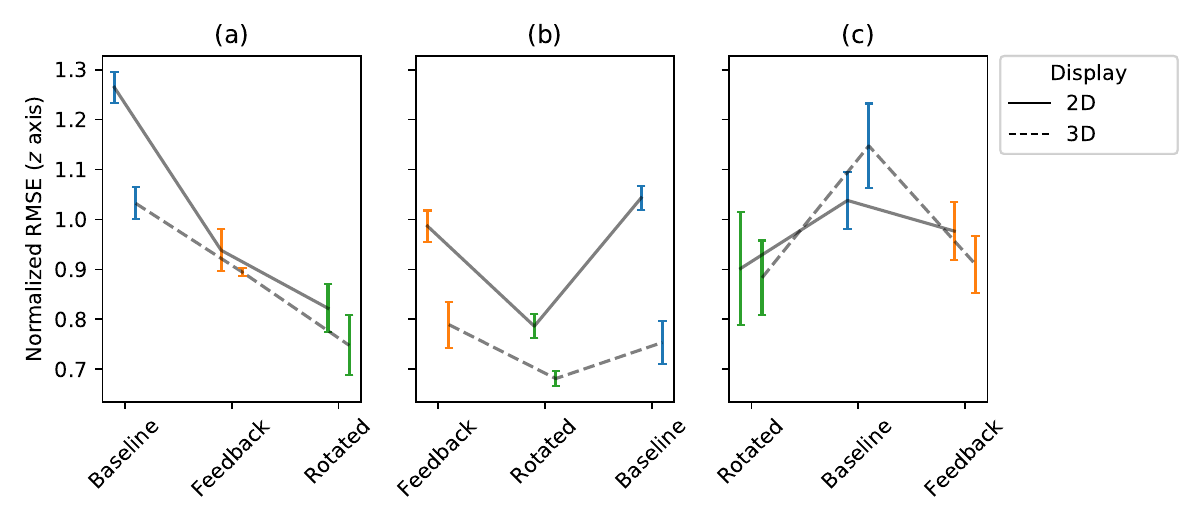
\includegraphics[height=7cm]{figures/AR/x_design_y_zrmse_col_startdesign_hue_device.png}
        \caption[The resulting normalized RMSE along the $z$ axis]{The resulting normalized RMSE along the $z$ axis. Subjects started in either the (a) Baseline, (b) Feedback, or (c) Rotated design.}
        \label{fig:zrmseanovas}
    \end{center}
\end{figure}

Results of the ANOVA on the $z$ axis RMSE showed significant effects for design ($F(2, 36)=84.92, p<.001$), device ($F(1, 18)=7.22, p<0.015$), and start design ($F(2, 18)=4.81, p<0.021$).
The ANOVA also showed a significant interaction effect between design and starting design ($F(4, 36)=8.55, p<0.0001$), and a three way interaction between design, device, and starting design ($F(4, 36)=5.57, p<0.002$).
Further investigation into the effect of starting design using pairwise comparisons showed significance differences between subjects that started in the concurrent bandwidth feedback group and those in the baseline ($p<0.001$) or rotated ($p<0.001$) designs, but no difference between subjects that started in the baseline and rotated designs ($p>.38$).
The difference in performance between design, device, and starting design can be seen in Fig.~\ref{fig:zrmseanovas}.

Due to the unanticipated but significant interaction effects in the starting design factor, the remainder of the analysis is split between subjects who started with the concurrent bandwidth feedback design and those that did not (e.g., those that started in the baseline or rotated design).
For subjects that started in the CBF design, there was a significant effect of design ($F(2, 12)=21.65, p<.0001$), a significant effect of display ($F(1, 6)=36.73, p<0.001$), and a significant interaction effect between design and device ($F(2, 12)=5.42, p<0.021$).
For subjects that did not start in the CBF design, there was a significant effect of design ($F(2, 28)=38.70, p<.0001$), but no significant effect or display ($F(1, 14)=1.03, p>0.32$), and no interaction effect ($F(2, 12)=0.03, p>0.97$).
The resulting difference between subjects who started in the CBF design and those who did not is presented in Fig.~\ref{fig:zrmseanovas2}.
For subjects who did not start in the CBF design, display had no significant effect, and subjects performed best in the rotated design, followed by the feedback design and finally the baseline design.
Subjects who started in the CBF design performed significantly better in the 3D display than the 2D displays, and performed best in the rotated design, but comparably between the feedback and baseline designs.

\begin{figure}[tb!]
    \begin{center}
        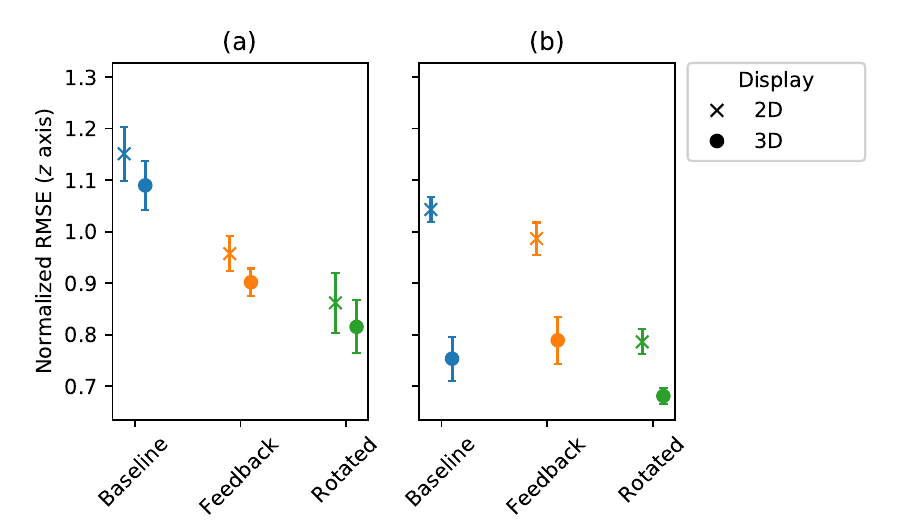
\includegraphics[height=7cm]{figures/AR/x_design_y_zrmse_hue_device_col_cbf_first.png}
        \caption[The resulting normalized RMSE along the $z$ axis]{The resulting normalized RMSE along the $z$ axis, grouping by subjects that started (a) without or (b) with feedback.}
        \label{fig:zrmseanovas2}
    \end{center}
\end{figure}

The NASA-TLX was used to measure differences in subjective workload, and the reaction time to the secondary task was used to measure differences in objective workload between design, device, and starting design.
There were no significant effects, nor interaction effects, found in the ANOVA for design, device, or starting design for the NASA-TLX measurements.
There was a significant effect of design ($F(2, 36)=7.93, p<0.0014$) for the reaction time to the secondary task, though the magnitude of this effect was very small between designs (less than 100 ms difference) and was not significant during Tukey HSD tests.
In general, there were no significant effects found for workload measurements.

\section{Discussions and Conclusion}
To summarize these results, there were significant effects found in the $z$ axis RMSE for design, with subjects generally performing the best using the rotated design, followed by the CBF design, and performing worst with the baseline design.
There were significant effects found for the factors of device and starting design, though these must be interpreted carefully.
Subjects who started with concurrent bandwidth feedback performed better than subjects who did not.
We believe that this result reinforces that found in our prior SAFER experiment, where subjects who were exposed to the CBF early on learned the task better than those who were not exposed~\citep{karasinski_real-time_2017,karasinski_development_2016,karasinski_real-time_2016}.
An interesting effect of this exposure is that, after learning the task with CBF, subjects continued on to perform significantly better in the baseline condition than those subjects that did not start in the CBF design.

Subjects who started in the CBF design and who were wearing the HoloLens appear to have used the CBF to better learn the depth cue presented in the stereoscopic display.
These subjects continued to perform significantly better than subjects who started with the CBF design but without the stereoscopic display when they continued to the baseline design.
This indicates that even a brief exposure to the concurrent bandwidth feedback was sufficient to induce improved performance in the baseline design.
Additionally, this also suggests that well trained subjects could perform better using the stereoscopic display compared with the traditional display, but that subjects who were still learning the task could not take advantage of the additional depth cues provided by the display.
Finally, there were no significant effects found for the NASA-TLX measurements, and there were significant but small effects found between the designs for reaction time.

In summary, we find partial agreement with all of our hypotheses in respect to the performance aspects of our experiment, while the workload was essentially unaffected by all of our experimental factors.
For Hypothesis 1, subjects who completed the baseline design before the CBF design performed better in the CBF design, while subjects who completed the CBF design before the baseline performed approximately the same in both designs.
This indicates that CBF can both improve performance compared to a baseline design, and better train subjects such that, even after brief exposure, the feedback is no longer required.
Workload was unaffected by the CBF.
For Hypothesis 2, subjects who started in the CBF design appear to have better learned the task and used the CBF to learn to interpret the depth cue provided by the stereoscopic display.
Subjects who were not initially exposed to this feedback were unable to exploit the display, and did not perform significantly better than subjects without the display.
For Hypothesis 3, subjects in the rotated design did perform better than those in the baseline design and appeared to be able to use this view to better interpret the depth of the target.

These results suggest that 3D displays such as the HoloLens have the potential to improve performance, but that simply donning a 3D display is not in itself wholly sufficient for improvement.
Subjects performed the tracking task better when we exposed them to CBF early in the experiment, and were able to use the depth cues provided by the 3D display to sustain this improvement when the feedback was removed.
These subjects achieved the best performance that we observed in this experiment, suggesting that the combination of CBF and 3D displays is an effective training technique for optimal performance.
The rotated design generally resulted in excellent performance by all subjects, which suggests that a direct ($\theta=0$) view should be avoided for three-axis tracking tasks.
Care must be taken to provide subjects with the feedback required to adequately complete the task, and subjects should not expect to perform better simply because they have 3D displays.

% \section*{Acknowledgments}
% The authors would like to thank all the subjects for volunteering to take part in the study.
% This work was supported by the Link Foundation's Modeling, Simulation, and Training Fellowship.

\chapter{Conclusion}
\label{chap:conclusion}

\textbf{\color{red} This chapter does not yet exist.}

\section{Research Questions}

In Chapter~\ref{sec:intro_questions}, we listed seven research questions that we aimed to answer by this research.
Here we summarize our answers to these questions.

\section{Future Work}



% note that the 'plainnat' style does not allow URL's in the bibtex entry
%
% some ideas here:
% http://bib2web.djvuzone.org/bibtex.html
%

% reset the page style
\pagestyle{plain}

\ssp
\bibliography{dissertation}


% To enable this it will need to be added to toc so it's not in a chapter
%\nocite{*}
%\printbibliography %[heading=bibliography]

% the appendix:
% there are several sections, that don't really fit into the main chapters
%
\part*{\addcontentsline{toc}{part}{Appendices}Appendices}
\appendix

% reset page style to fancy
%\pagestyle{fancyplain}

\chapter{Trade Analysis Tables} \label{appendix:trade-tables}

\begin{figure}[b!]
    \begin{center}
        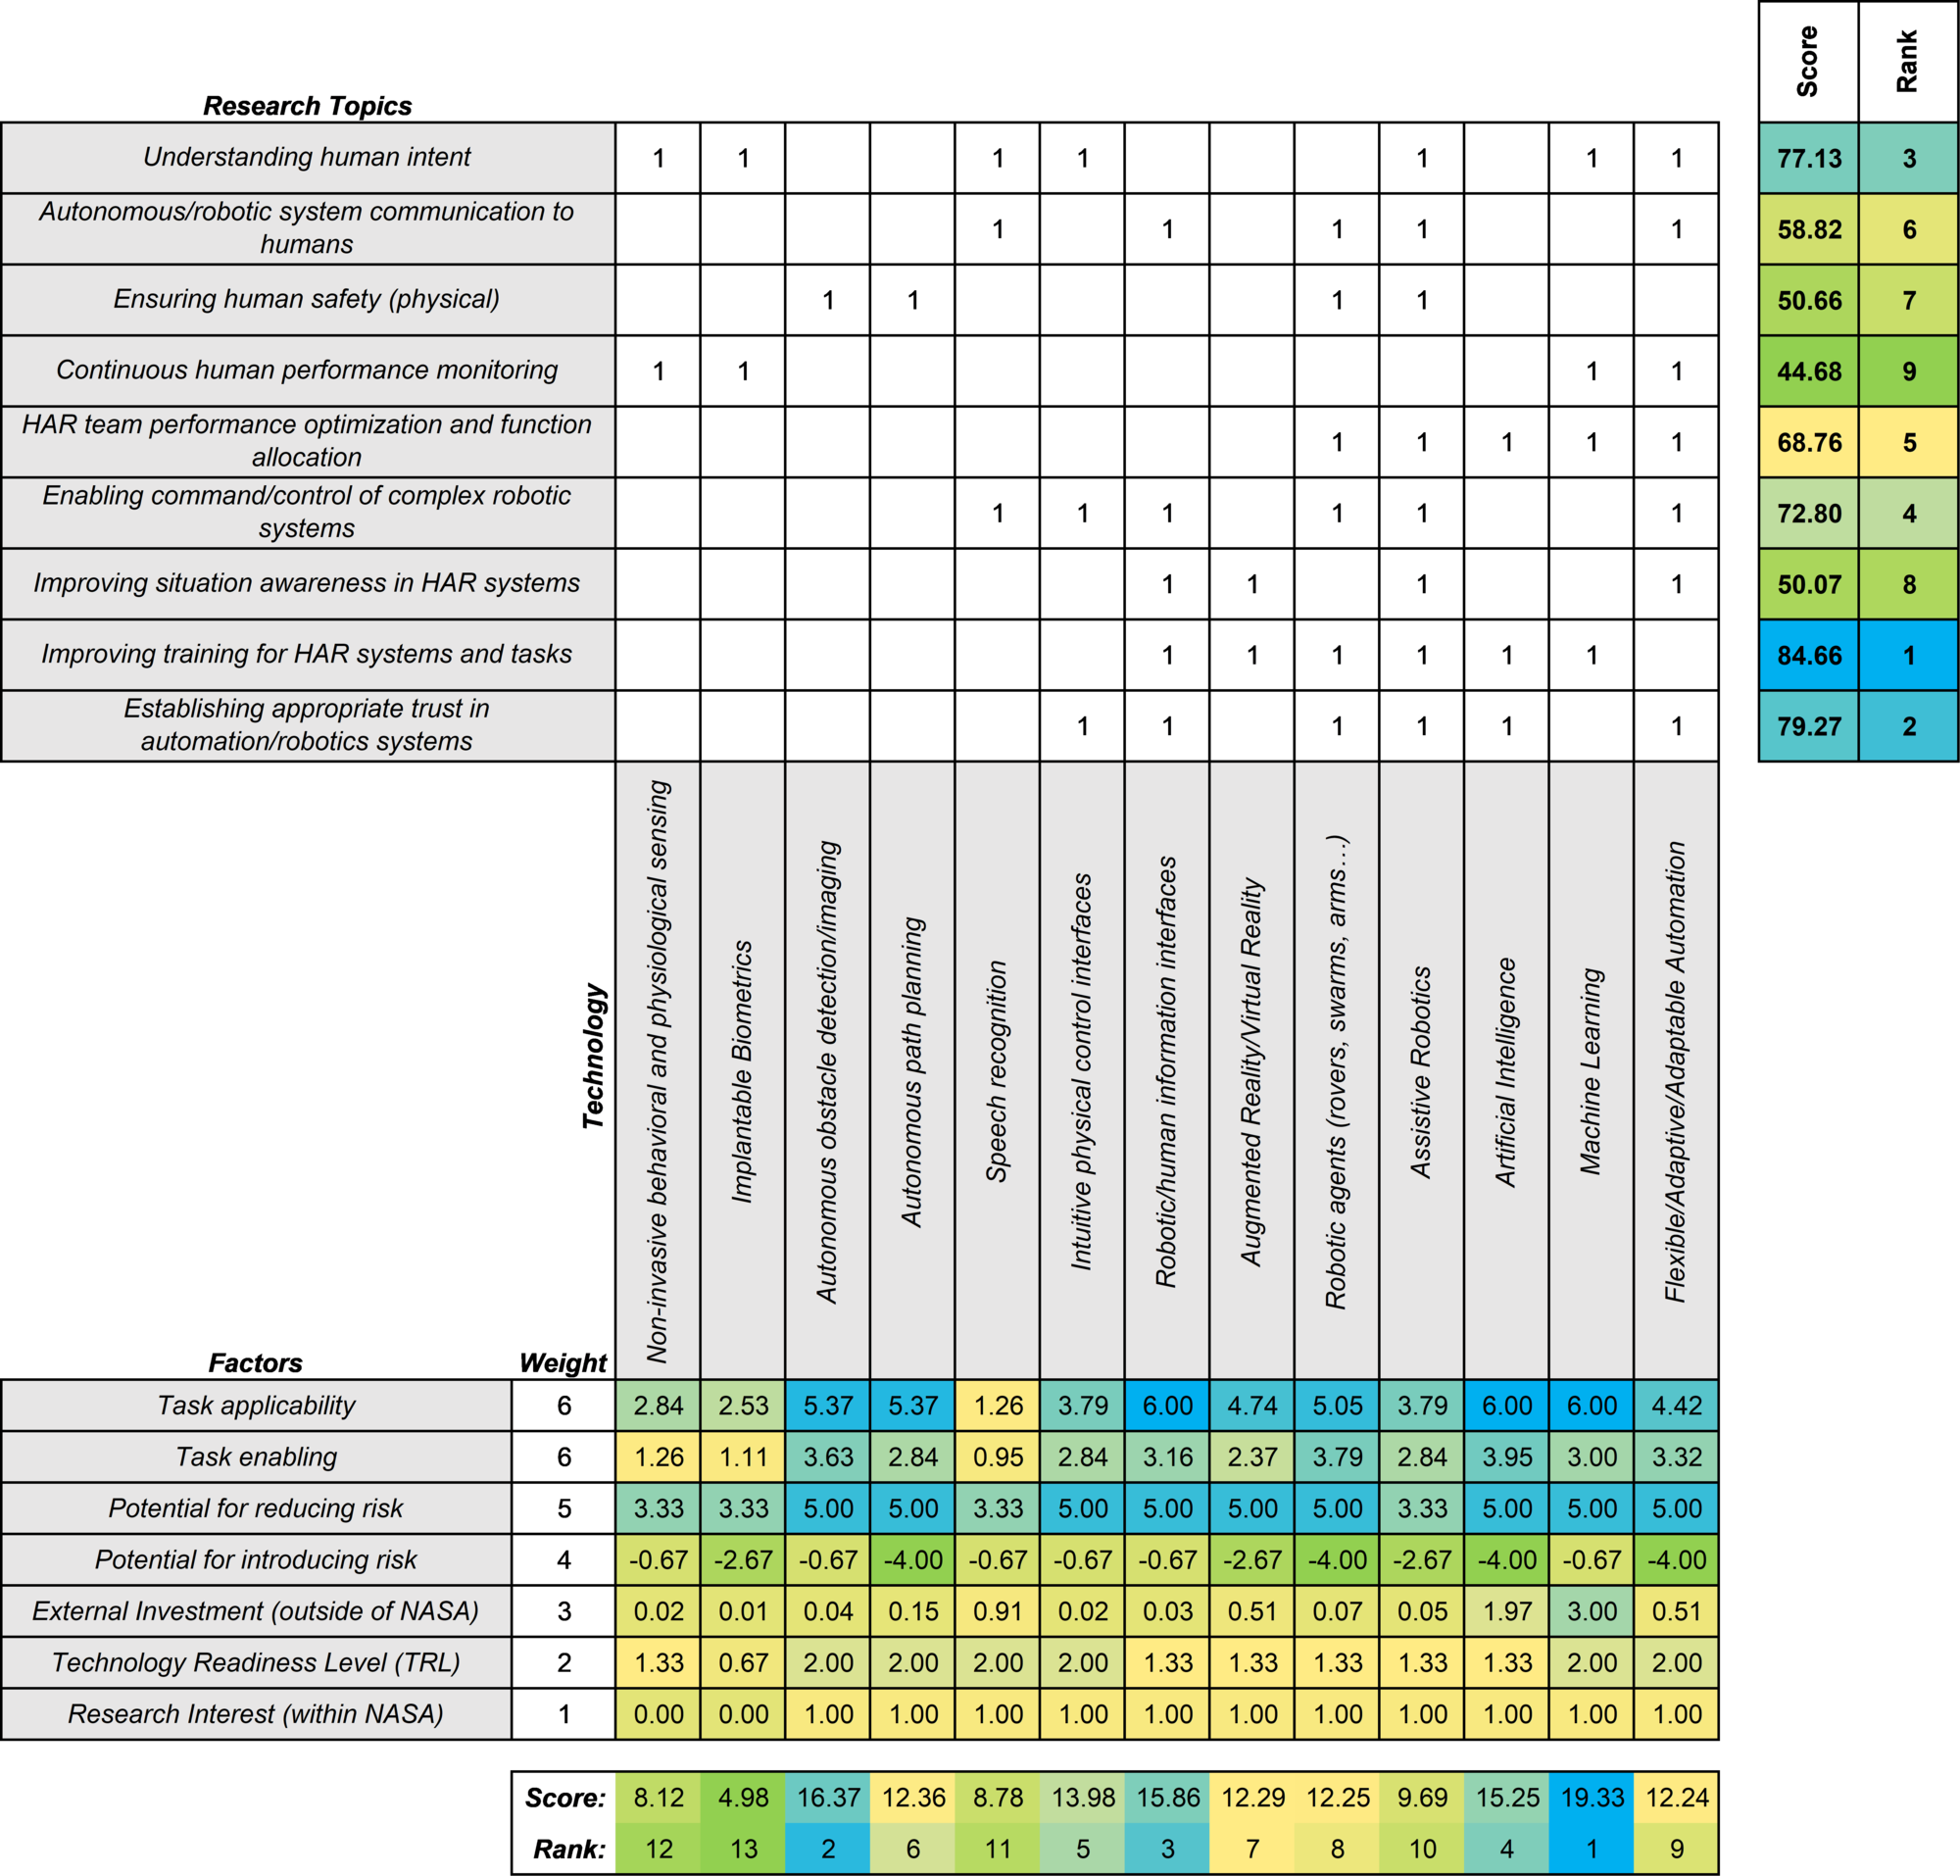
\includegraphics[width=0.8\linewidth]{figures/TradeStudy/figurea1.png}
        \caption[Top-level trade table]{Top-level trade table with final research topic scores (top right), final technology scores based on factors (bottom) and weighted factor-level scores for each technology.}
        % \label{figure:}
    \end{center}
\end{figure}

\begin{figure}[b!]
    \begin{center}
        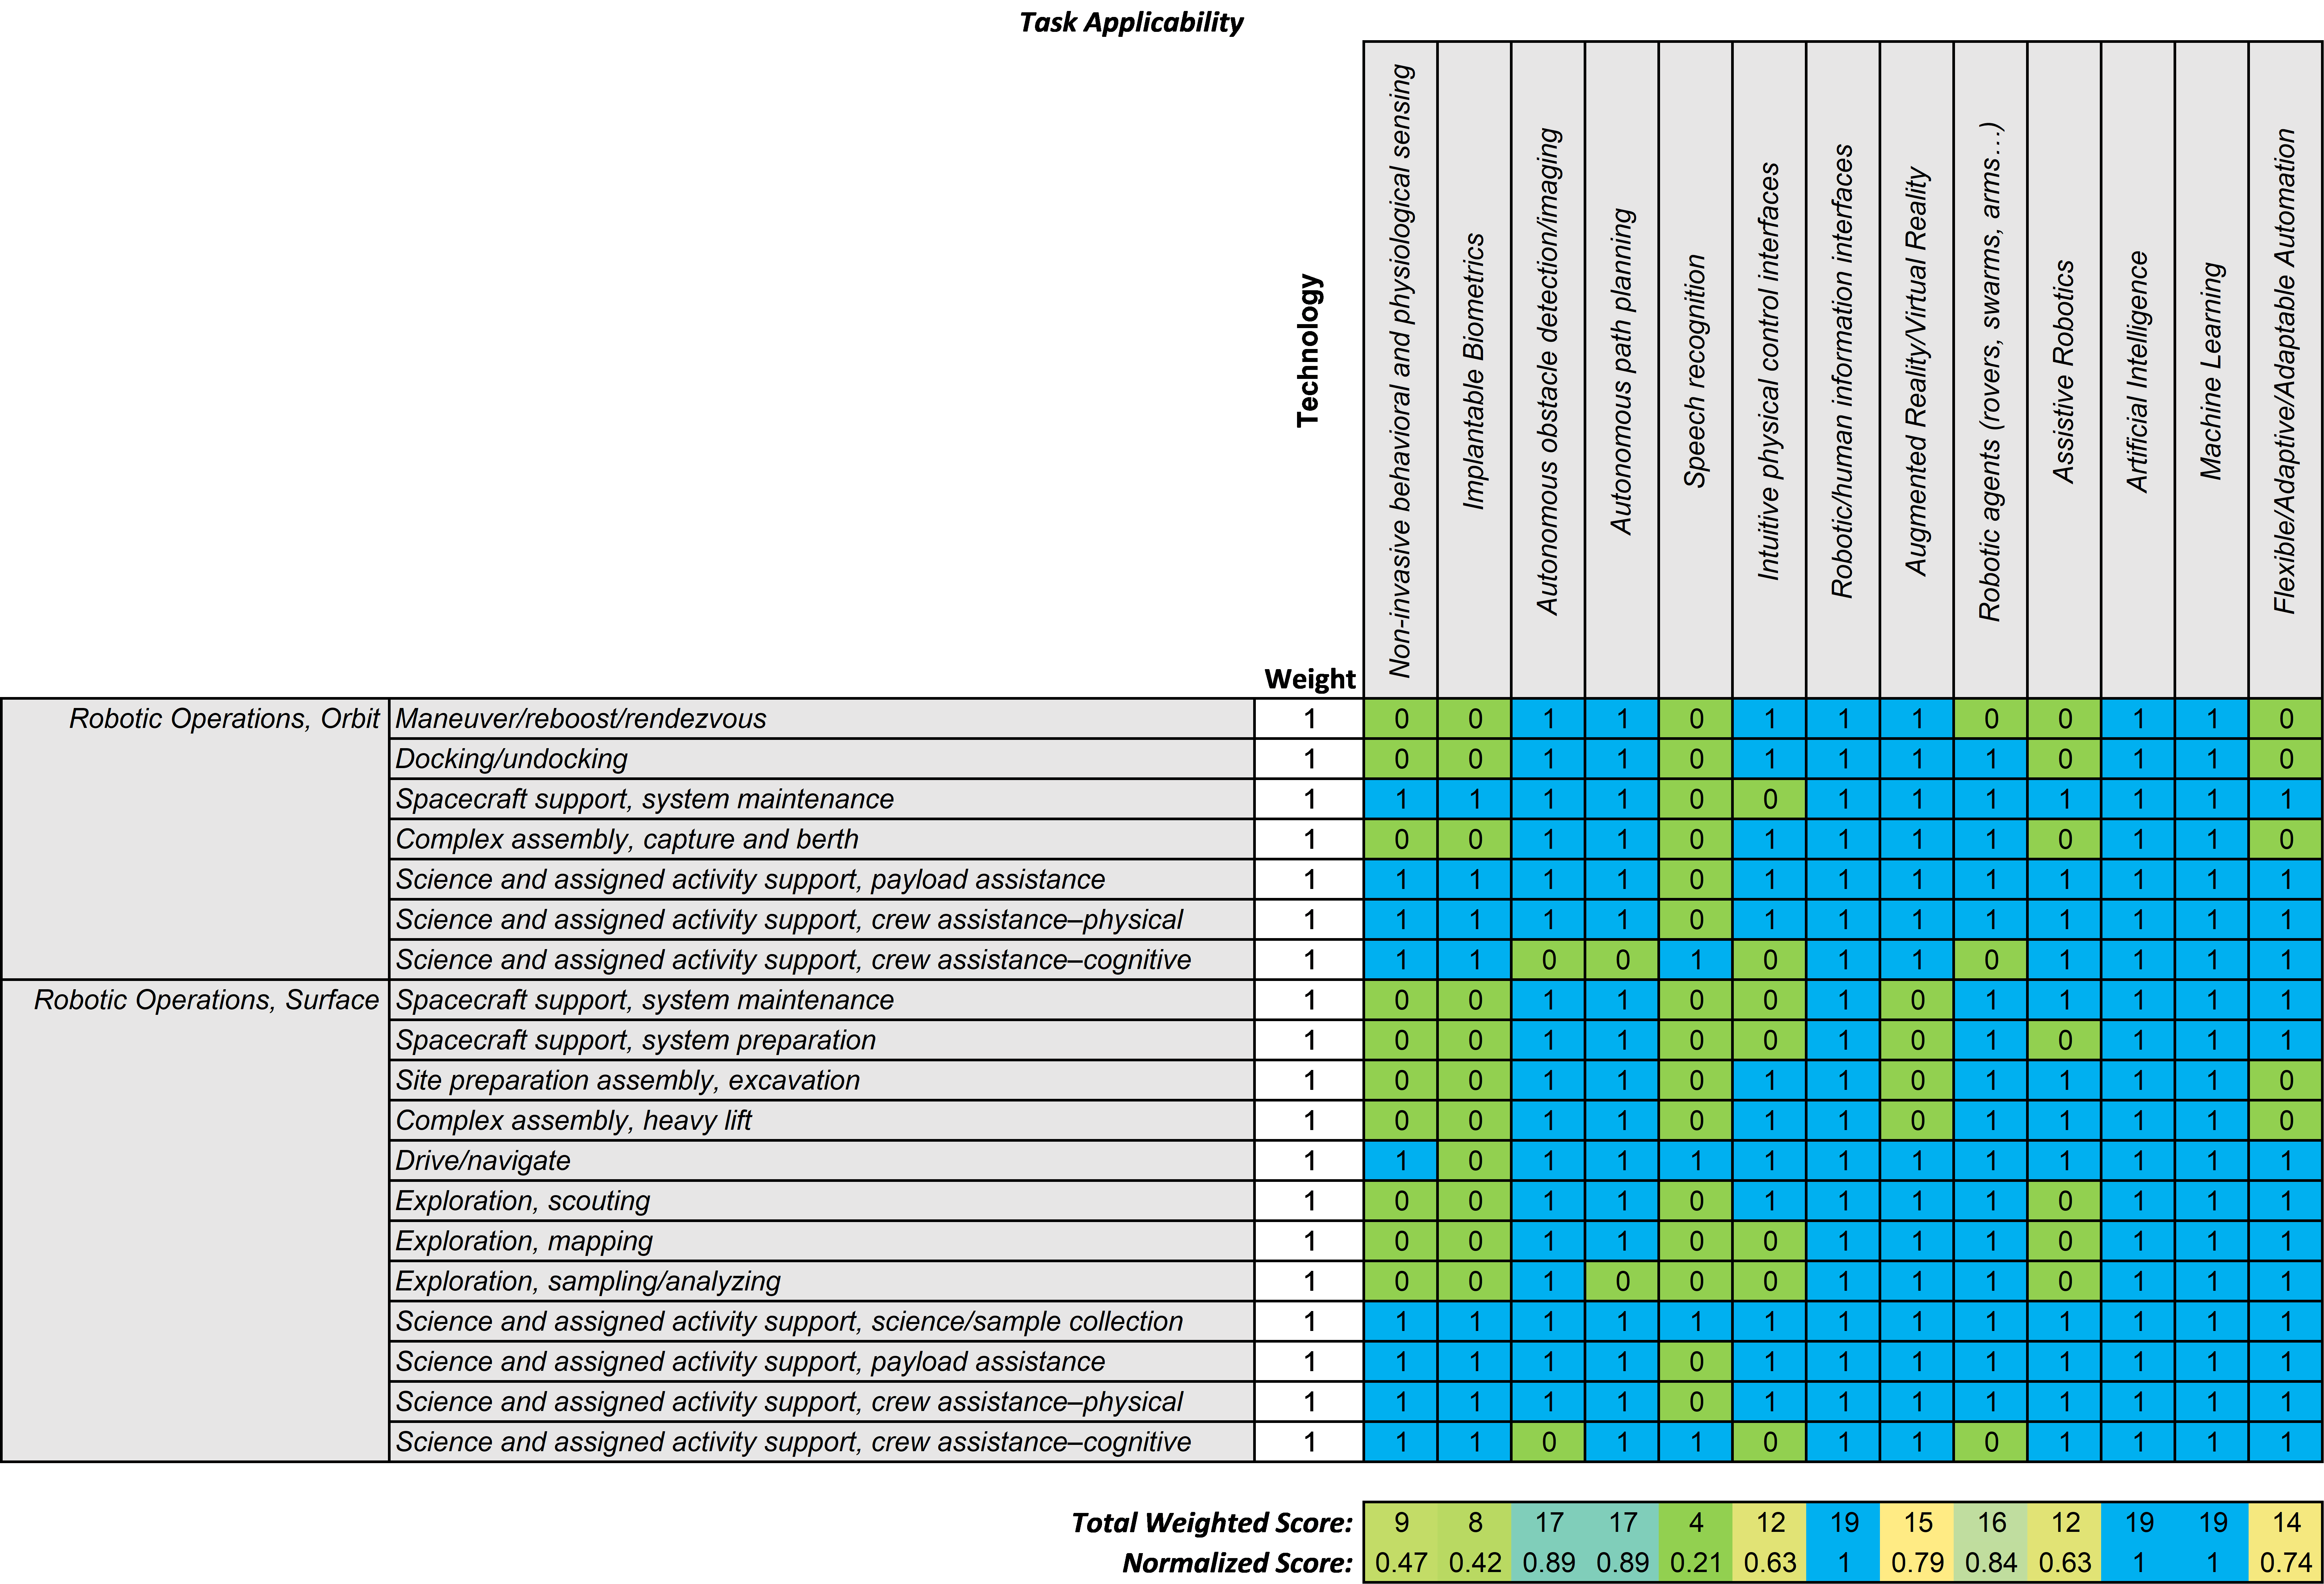
\includegraphics[width=0.8\linewidth]{figures/TradeStudy/figurea2.png}
        \caption[Technology to Task Applicability factor-level trade table]{Technology to Task Applicability factor-level trade table.}
        % \label{figure:}
    \end{center}
\end{figure}

\begin{figure}[b!]
    \begin{center}
        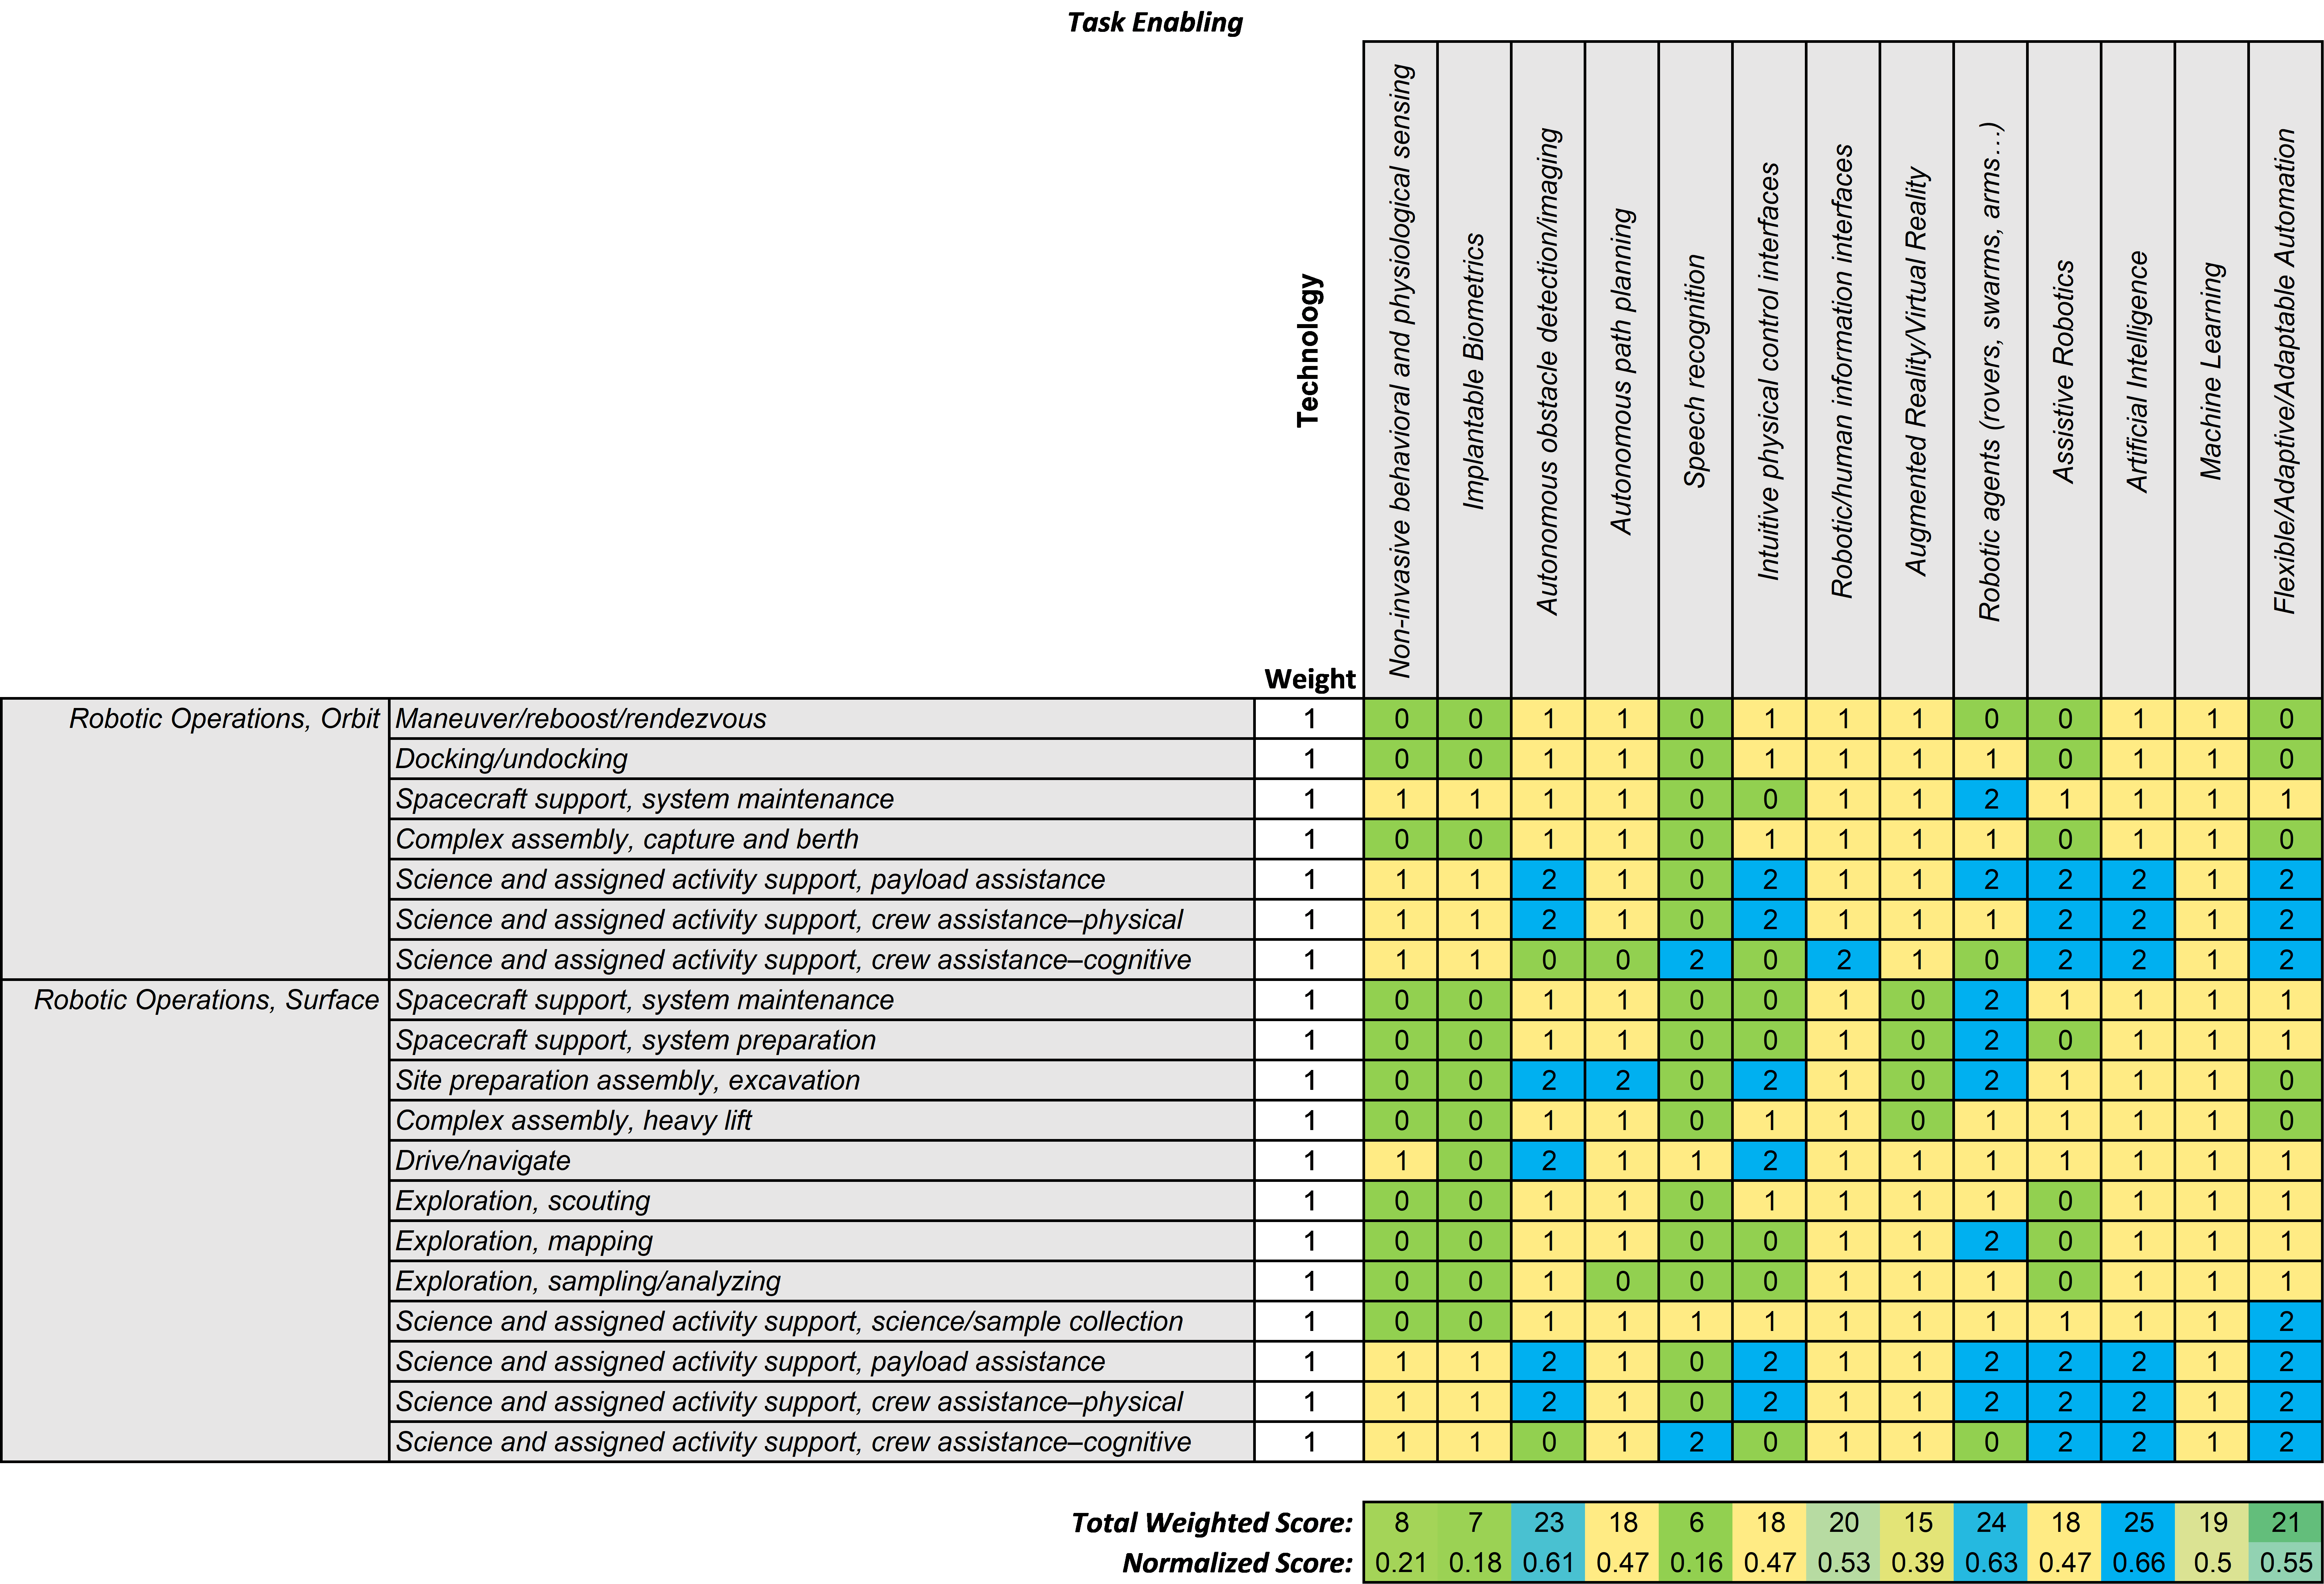
\includegraphics[width=0.8\linewidth]{figures/TradeStudy/figurea3.png}
        \caption[Technology to Task Enabling factor-level trade table]{Technology to Task Enabling factor-level trade table.}
        % \label{figure:}
    \end{center}
\end{figure}

\begin{figure}[b!]
    \begin{center}
        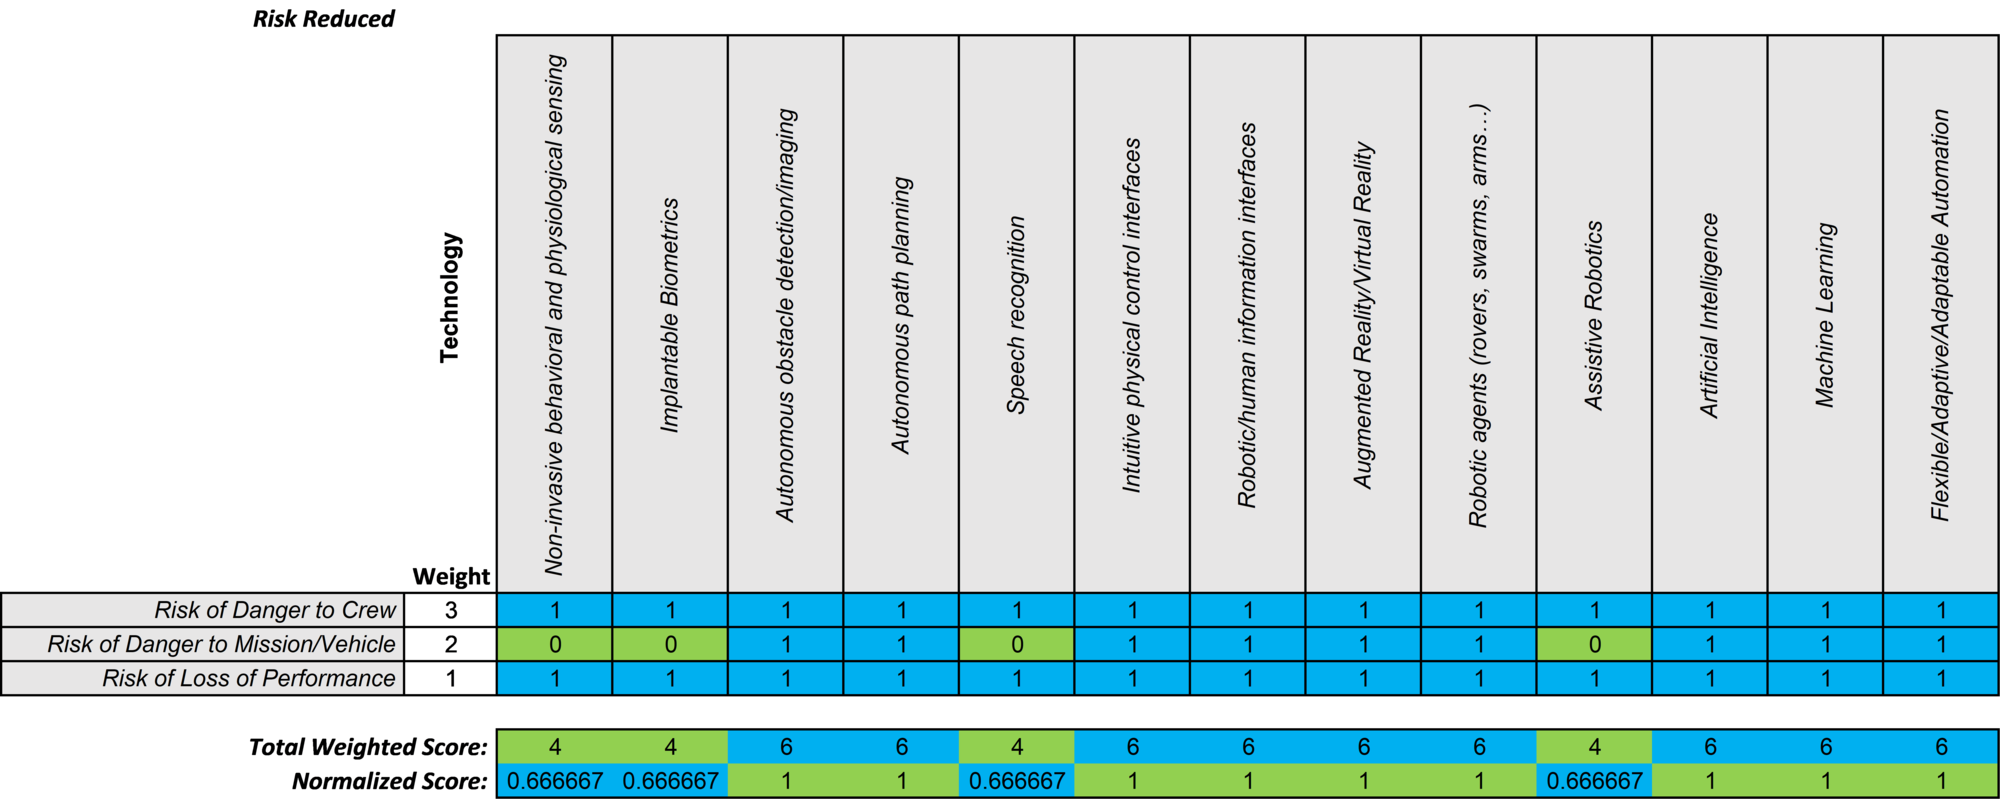
\includegraphics[width=0.8\linewidth]{figures/TradeStudy/figurea4.png}
        \caption[Technology to Risk Reduced factor-level trade table]{Technology to Risk Reduced factor-level trade table.}
        % \label{figure:}
    \end{center}
\end{figure}

\begin{figure}[b!]
    \begin{center}
        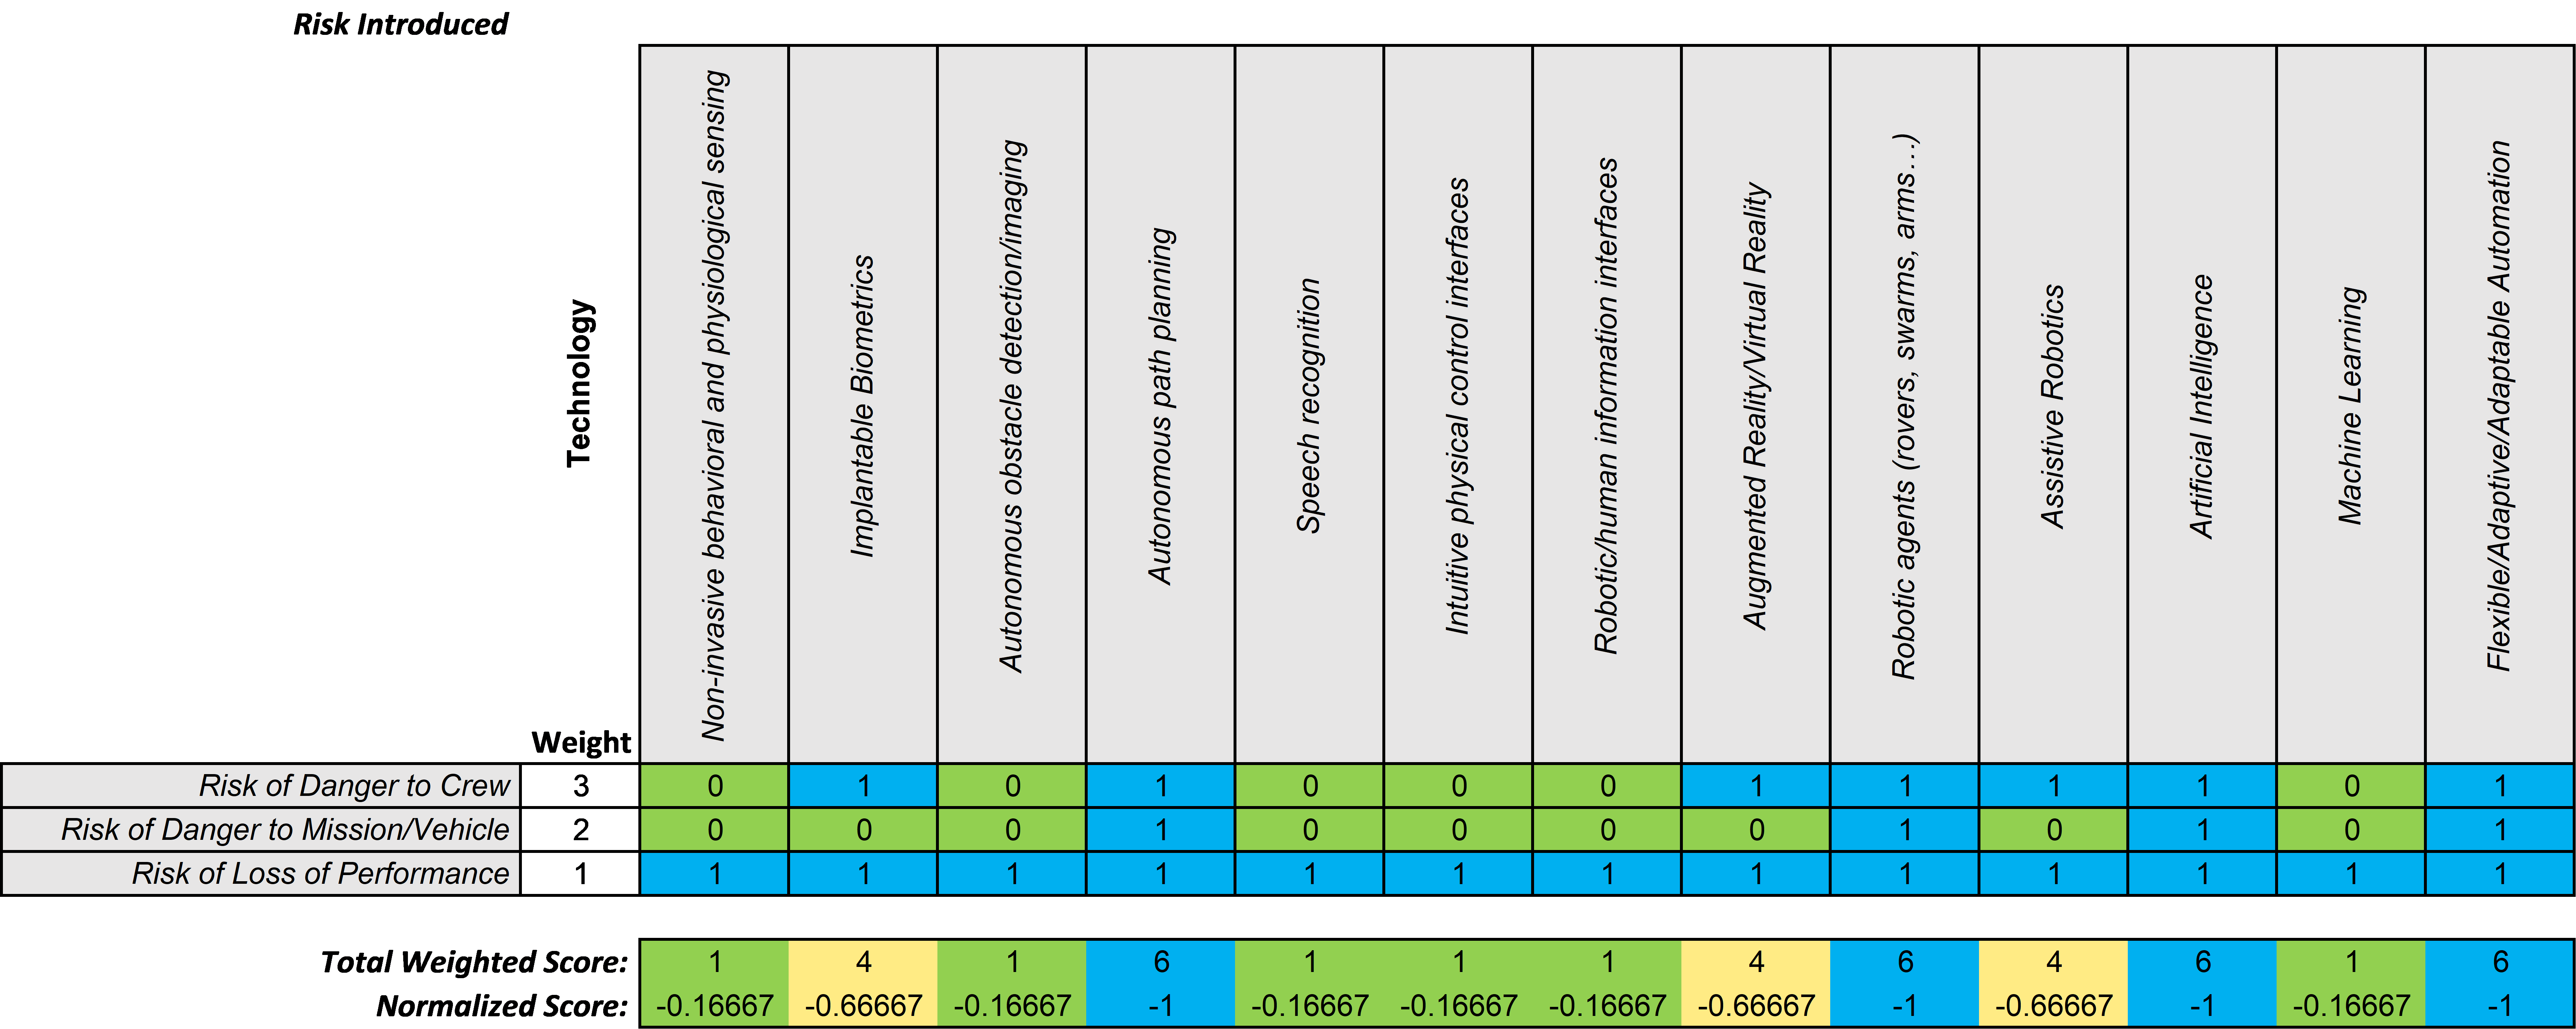
\includegraphics[width=0.8\linewidth]{figures/TradeStudy/figurea5.png}
        \caption[Technology to Risk Introduced factor-level trade table]{Technology to Risk Introduced factor-level trade table.}
        % \label{figure:}
    \end{center}
\end{figure}

\begin{figure}[b!]
    \begin{center}
        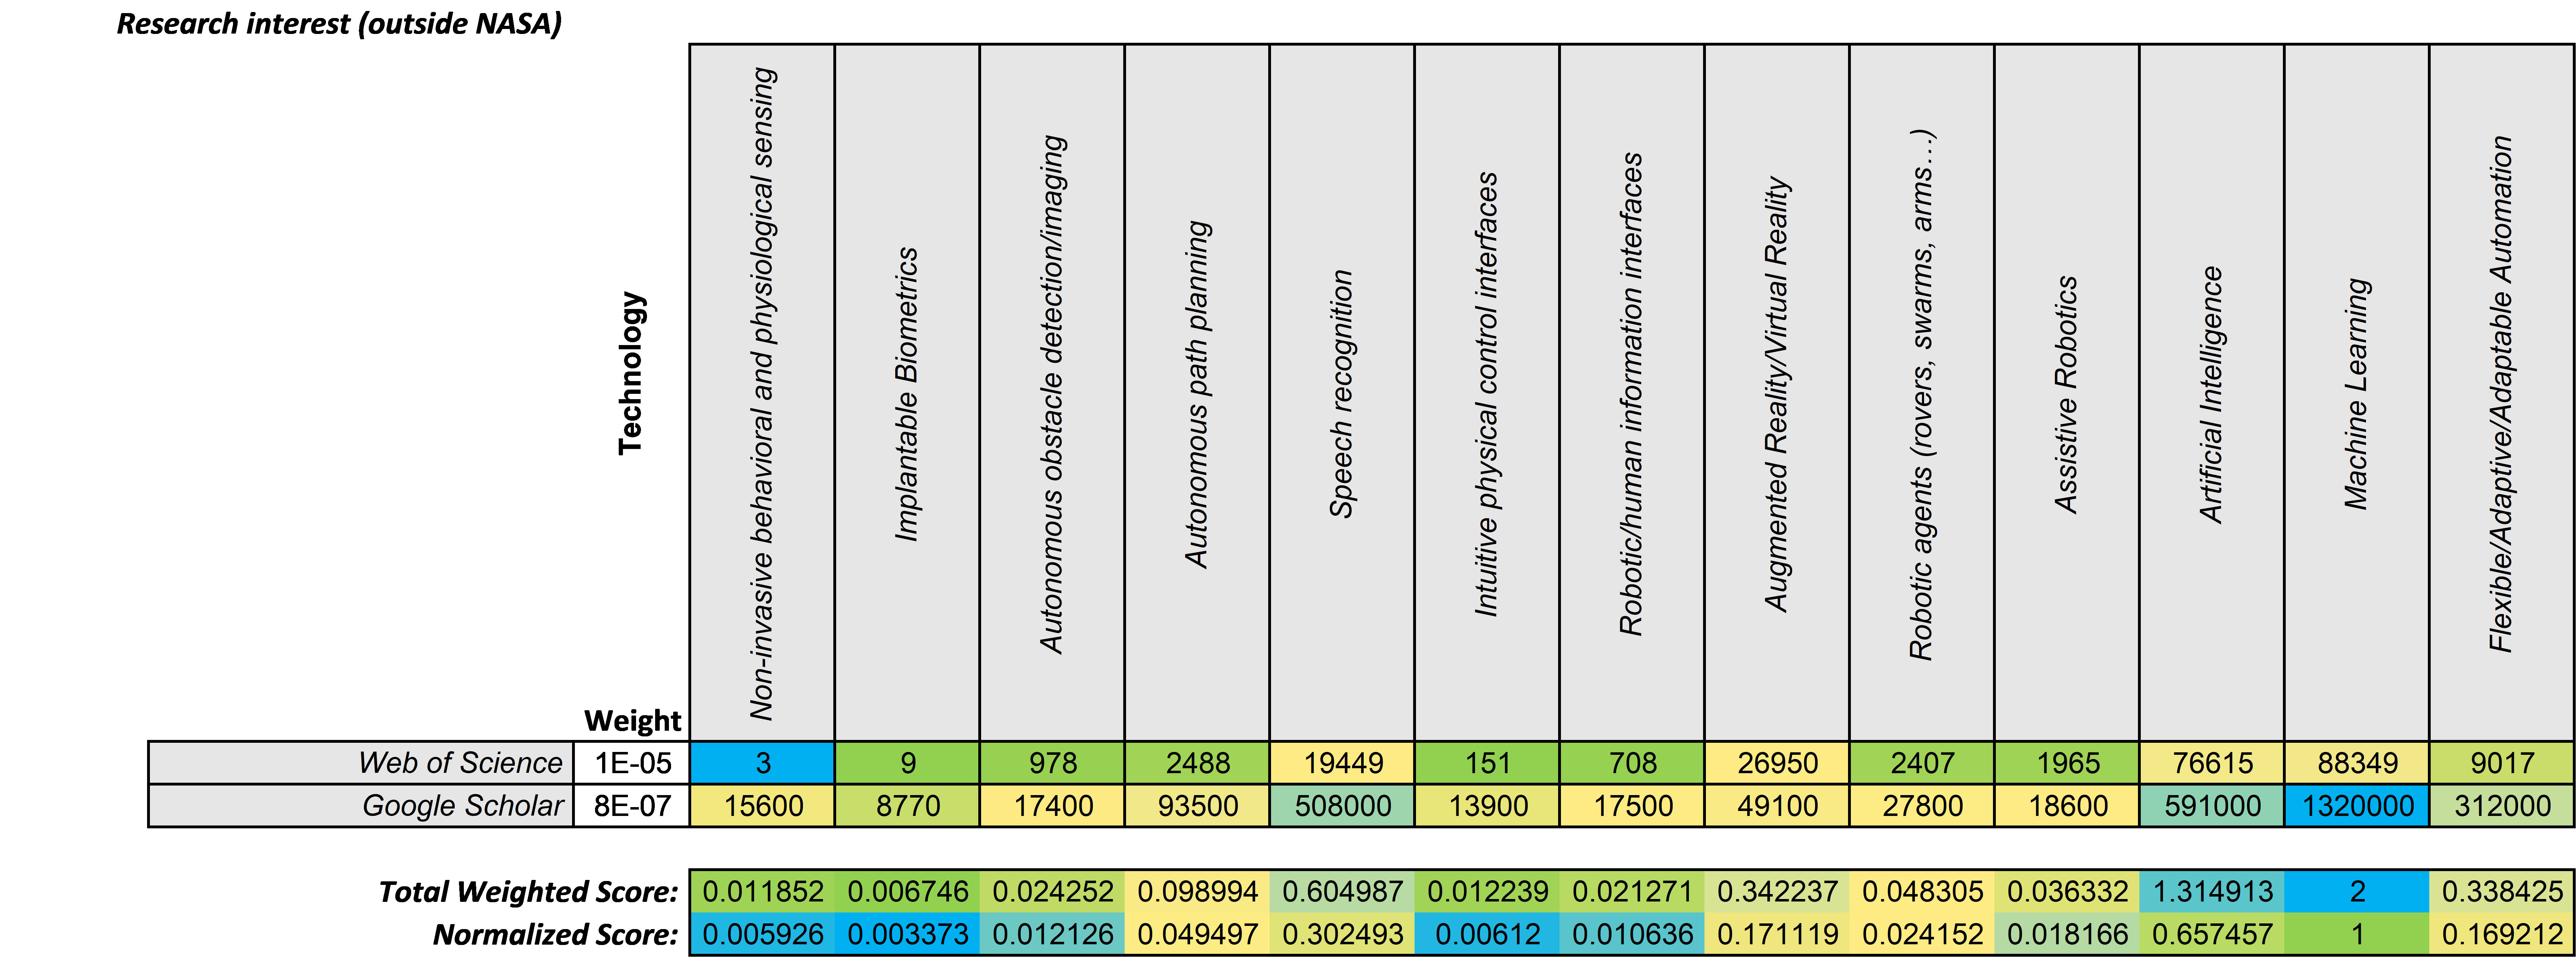
\includegraphics[width=0.8\linewidth]{figures/TradeStudy/figurea6.png}
        \caption[Technology to Research Interest (outside NASA) factor-level trade table]{Technology to Research Interest (outside NASA) factor-level trade table.}
        % \label{figure:}
    \end{center}
\end{figure}

\begin{figure}[b!]
    \begin{center}
        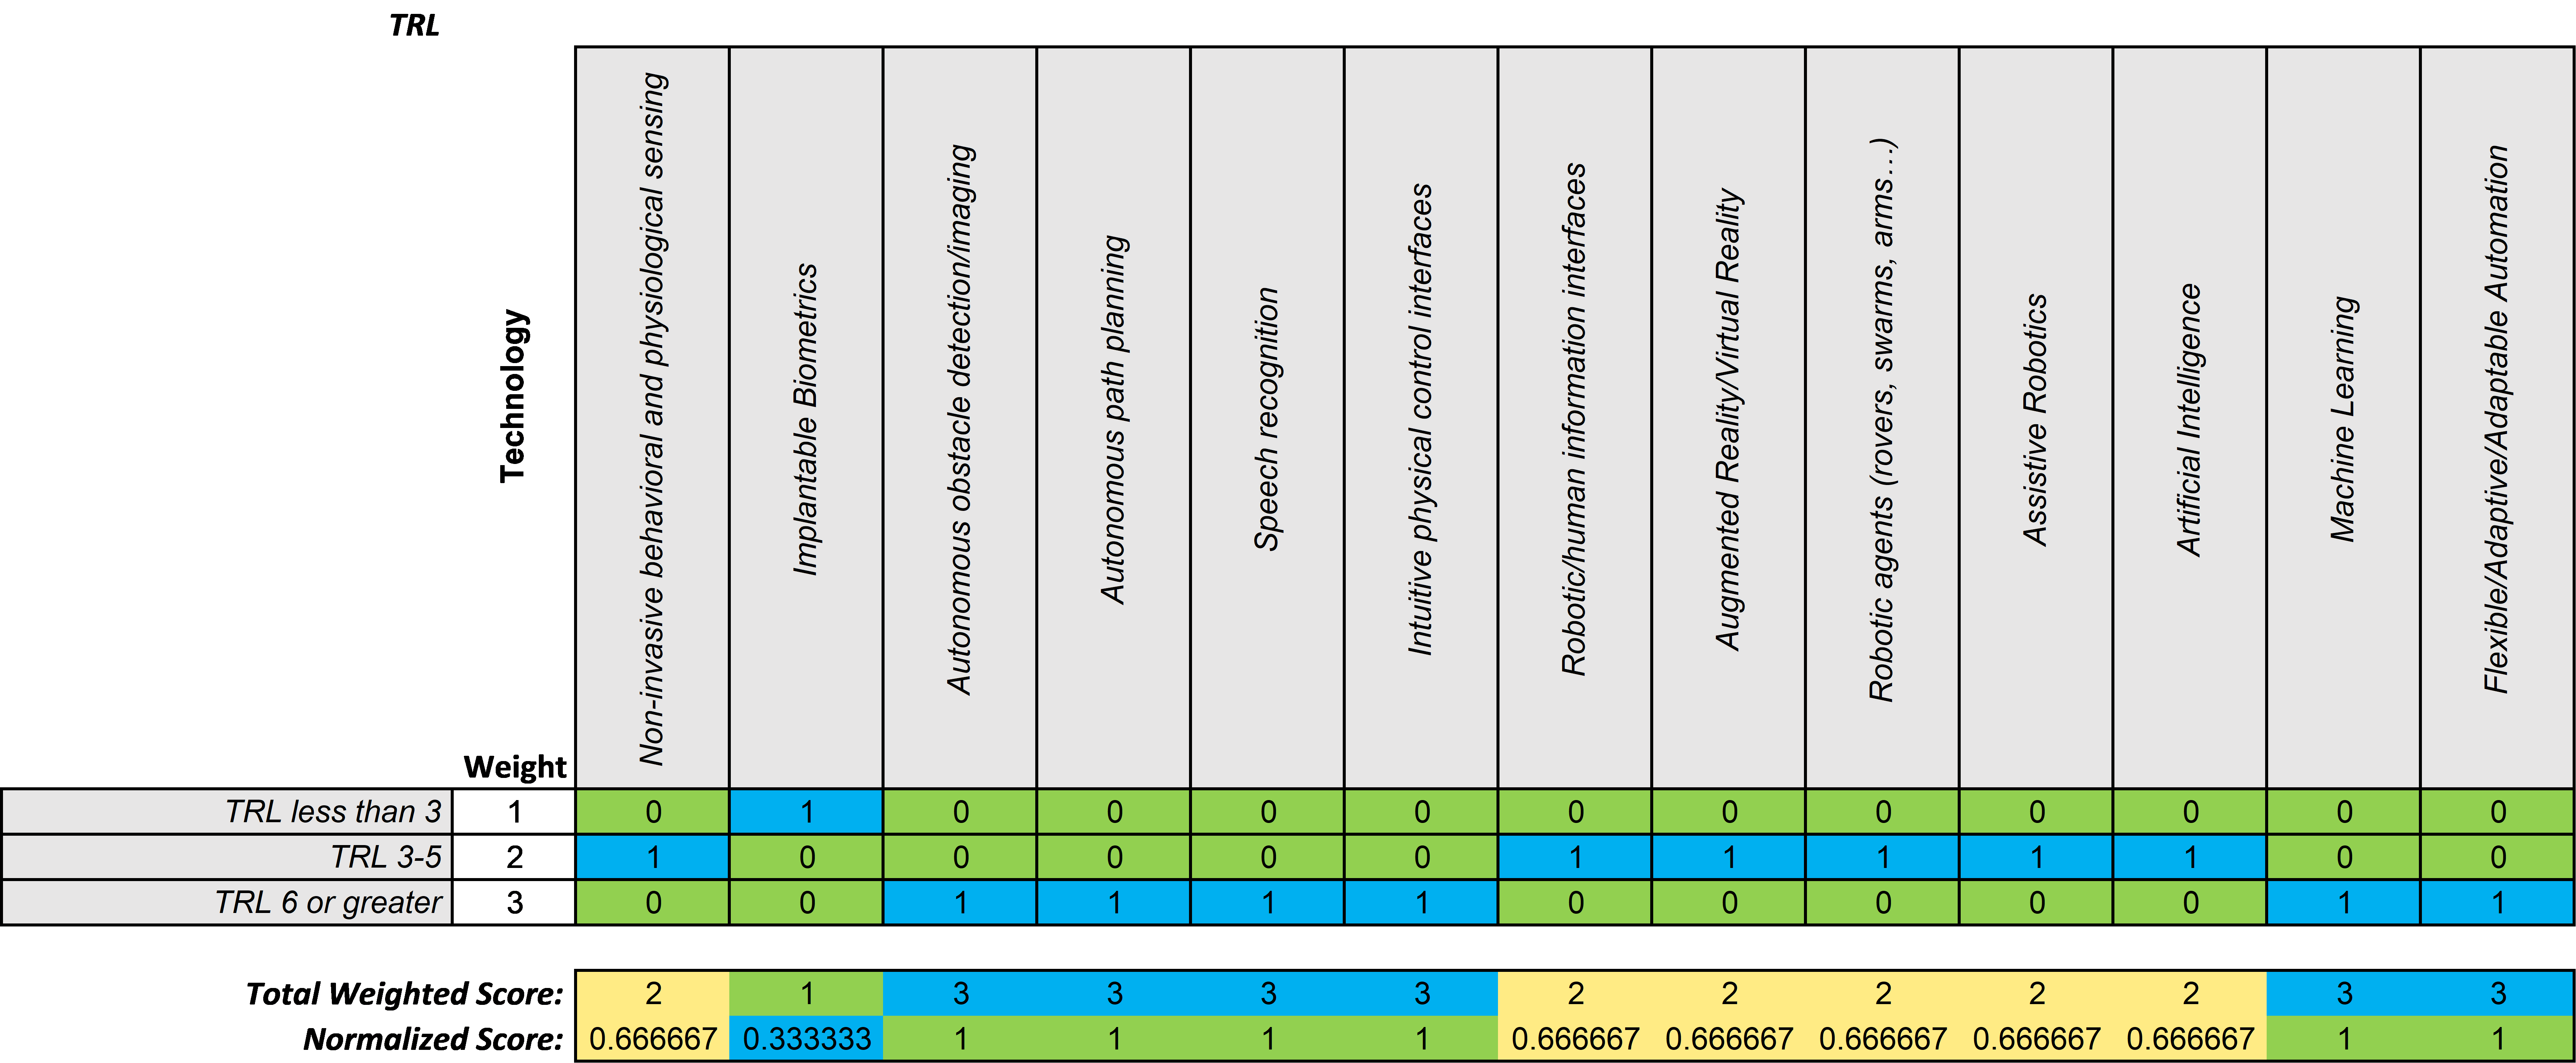
\includegraphics[width=0.8\linewidth]{figures/TradeStudy/figurea7.png}
        \caption[Technology to TRL factor-level trade table]{Technology to TRL factor-level trade table.}
        % \label{figure:}
    \end{center}
\end{figure}

\begin{figure}[b!]
    \begin{center}
        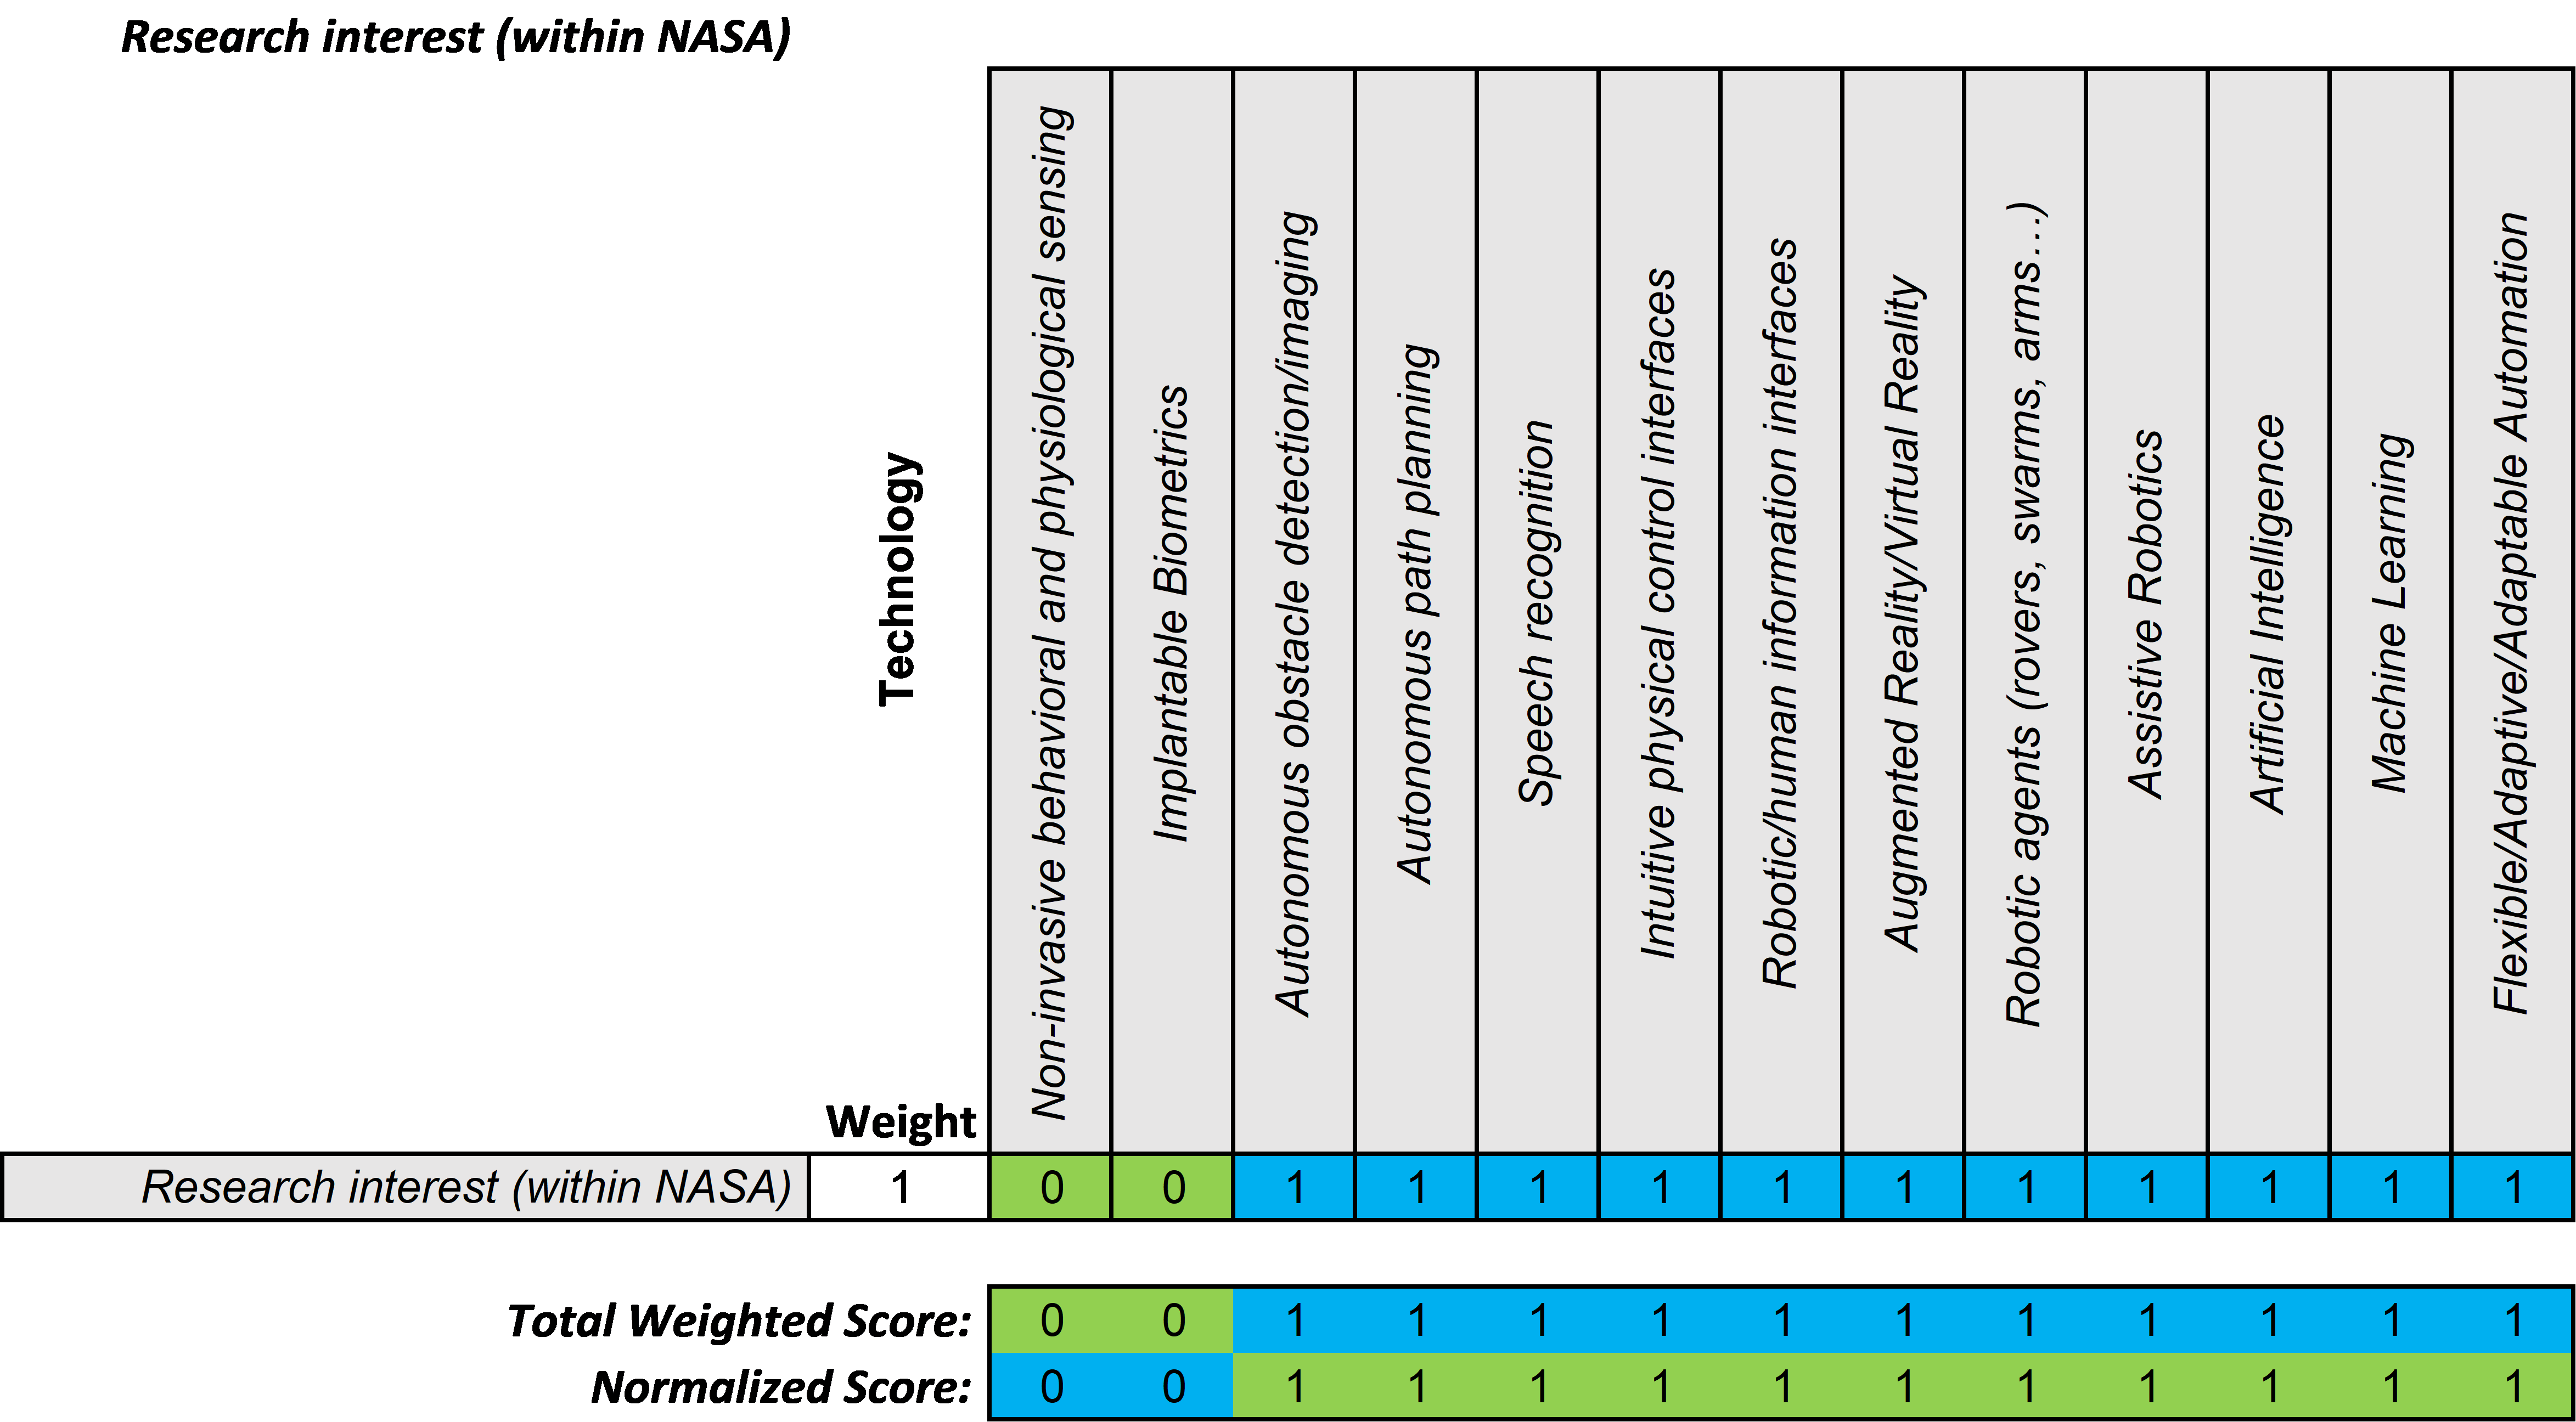
\includegraphics[width=0.8\linewidth]{figures/TradeStudy/figurea8.png}
        \caption[Technology to Research Interest (within NASA) factor-level trade table]{Technology to Research Interest (within NASA) factor-level trade table.}
        % \label{figure:}
    \end{center}
\end{figure}

% Appendix B: Subject Matter Expert Summary of Backgrounds
% The SMEs interviewed to gather background information on the HARI trade space all have extensive experience in either HAR integration research, human factors, or both, in their respective fields. Additionally, three SMEs have experience in related fields: one person in data analytics, and two others in psychology/neuroscience. The SMEs have a wide range of experience addressing different research applications, captured in Table B1.

% SME	Background	Expertise
% 		Space	Aviation	Military	Medical	Automotive	Locomotive	Robotics (general)
% 1	Industry		x	x
% 2	Industry		x	x
% 3	Academia	x	x			x	x	x
% 4	Industry,
% Former NASA	x	x		x
% 5	Military			x	x			x
% 6	Academia, Industry				x	x
% 7	Academia	x	x	x			x
% 8	Academia,
% Industry		x					x
% 9	Academia	x			x			x
% 10	Industry,
% Former NASA	x			x	x
% Table B1: Background and application area expertise of interviewed subject matter experts

% Appendix C: Annotated Bibliography
% Parasuraman, Raja, and Christopher D. Wickens. "Humans: Still vital after all these years of automation." Human factors 50.3 (2008): 511-520.
% 	In their 2008 review, Parasuraman and Wickens discuss major discoveries and developments in levels and stages of automation, reliance on and compliance with automation, and adaptive automation. "Parasuraman, Sheridan, and Wickens (2000) accordingly proposed an extension of the LOA concept to four information-processing stages: (a) information acquisition, (b) information analysis, (c) decision making, and (d) action, with each stage having its own LOA scale (for similar scales, see Endsley & Kaber, 1999; Endsley & Kiris, 1995)."
% Ososky, Scott, et al. "Building Appropriate Trust in Human-Robot Teams." AAAI Spring Symposium: Trust and Autonomous Systems. 2013.
% 	In their 2013 paper, Ososky et al. describe autonomous, intelligent robots as teammates, rather than tools, and describe the importance of appropriate, rather than maximal, trust in the human-robot team. They discuss how human operators must create a sufficiently developed mental model of a robot to appropriately use it for tasks which the robot can perform superiorly to the human. They note that inaccurate mental models can create "pitfalls for robotic system misuse or disuse", and that accurate mental models are required for the human to appropriately trust the robot. They argue that appropriate trust in the robotic system leads to how the robotic system is ultimately used.
% Beer, Jenay M., Arthur D. Fisk, and Wendy A. Rogers. "Toward a framework for levels of robot autonomy in human-robot interaction." Journal of Human-Robot Interaction 3.2 (2014): 74-99.
% 	In their 2014 paper, Beer, Fisk, and Rogers outline a framework for levels of robot autonomy (LORA) for human-robot interaction (HRI), with the goal of allowing researchers to identify the impacts of autonomy on the interaction between human and robot. They outline a set of guidelines which can serve as "(1) a set of guidelines suggesting task and environmental influences on robot autonomy, (2) guidelines for determining or measuring autonomy, (3) a taxonomy for categorizing autonomy, and finally, (4) a set of HRI variables that may be influenced by robot autonomy."
% Chen, Jessie YC, and Michael J. Barnes. "Human–agent teaming for multirobot control: A review of human factors issues." IEEE Transactions on Human-Machine Systems 44.1 (2014): 13-29.
% 	In their 2014 paper, Chen and Barnes identified important human factors issued related to human-agent teams in multirobot control. They conclude that agents acting as interfaces between human operators and intelligent systems are an efficient way for operators to supervise multiple systems, while natural language processing is not required, the agents must have the ability to recognize operator intent, and that mixed initiative architectures can take advantage of both the human's expertise and the agent's precision and ability to act quickly. Mixed initiative systems, a subset of flexible automation, which allows for a dynamic level of automation based on the operator's state and events in the environment. Chen and Barnes further note the importance of transparency in effectively calibrating operator trust in an autonomous system.
% Kehoe, Ben, et al. "A survey of research on cloud robotics and automation." IEEE Trans. Automation Science and Engineering 12.2 (2015): 398-409.
% 	Kehoe et al.'s 2015 paper considers robots and automation systems that rely on externally networked support, and focuses on the benefits of the cloud, including: big data, cloud computing, collective robot learning, and human computation. They note the state of the art in each of these areas while considering the current challenges and future directions research must should be taken. New issues associated with the rise in cloud technology include the need for techniques to consider time varying latency and quality of service, privacy concerns, and big data cleaning and filtering techniques. The note three levels at which a cloud computing framework are currently established: Infrastructure as a Service (IaaS), where bare operating systems are available; Platform as a Service (PaaS), where more structure is provided, including access to application frameworks, databases, and programming languages; and Software as a Service (SaaS), where software is made available online rather than as a local service. They conclude by proposing a fourth cloud framework, Robotics and Automation as a Service (RAaaS), which merges PaaS and SaaS frameworks to provide a cloud service which processes inputs for robotics, suggests output actions, and monitors results to update future recommendations.
% Rautaray, Siddharth S., and Anupam Agrawal. "Vision based hand gesture recognition for human computer interaction: a survey." Artificial Intelligence Review 43.1 (2015): 1-54.
% 	Rautaray and Agrawal's 2015 survey provides a summary of progress in the field of vision-based hand gesture recognition and reviews the three main phases of hand gesture recognition: detection, tracking, and recognition. They analyze existing literature and note the required advances to further improve hand gesture recognition systems. They note the primary application domains of hand gesture recognition are desktop applications, followed by gaming and sign language. In terms of the challenges of operating in real-time and robustness, the authors find that comparisons are difficult as there is no commonly accepted baseline technique to compare to. Psychological aspects of gestures have been found to play an important role in hand gesture recognition systems. The authors find that, despite plenty of research into the field, 3D based gesture representations are still less preferred to appearance-based hand gesture representations.
% Ruhland, Kerstin, et al. "A review of eye gaze in virtual agents, social robotics and hci: Behaviour generation, user interaction and perception." Computer Graphics Forum. Vol. 34. No. 6. 2015.
% 	Ruhland et al.'s 2015 review covers the state of the art in generating artificial entities which include attempts to replicate the human eye, the role of social robotics, and the human-computer interaction issues involved. They found that research into eye-gaze models would greatly benefit from a fundamental foundation, and that individual differences in eye gaze are often ignored as research has traditionally attempted to model and recreate general behavior. Human-robot interaction in the field of eye gaze has largely focused on shared attention and gaze cueing, factors that have affected task performance and user speech. The authors note several challenges mapping virtual to physical robots, especially that robot expression has fewer degrees of freedom. They also, however, suggest that physical systems may be able to better direct human gaze to targets of interest in a real environment as they can avoid the Mona Lisa gaze effect associated with virtual agents.
% Yanco, Holly A., et al. "Analysis of human‐robot interaction at the darpa robotics challenge trials." Journal of Field Robotics 32.3 (2015): 420-444.
% 	Yanco et al.'s 2015 paper reviewed team performance at the DARPA Robotics Challenge (DRC) trials, analyzing the results, team structure, and human-robotic interfaces. The DRC trials were designed to test humanoid robots' ability to respond to disaster scenarios where communications bandwidth was limited or degraded. Yanco et al.'s team analyzed 8 of the 15 teams which volunteered to participate in their study, observing their team interaction and robot's performance during the challenge. They identified four areas required for teams to be successful in the challenge: robot mobility, robot manipulation, situation awareness of the robot and its surroundings, and an effective way to command the robot. They further found that the most effective team was successful largely due to their: increased sensor fusion, which reduced the operator's cognitive load and reduced the need to repeat tasks; decreased number of operators, which both increased situational awareness and decreased the amount of required operator input.
% Kolling, Andreas, et al. "Human interaction with robot swarms: A survey." IEEE Transactions on Human-Machine Systems 46.1 (2016): 9-26.
% 	Kolling et al.'s 2016 review is the first survey of human-swarm interaction, and presents the basics of swarm robotics, the cognitive needs of a swarm operator, and the challenges involved with providing a human-swarm interface. They break the cognitive complexity of the human-robot system into three difficulties, using an analogy of computational complexity: robots performing independent activities, with complexity O(n), which allows more robots to be controlled simply by adding more operators in a linear manner; robots interacting with other robots fully autonomously, with complexity O(1), which allows for a fixed number of robots to control any number of robots; and the case where robot-robot interaction must be controlled by an operator, with complexity O(>n), as the dependencies between robots results in more demand faster than the number of robots grows. Under the assumption that O(1) complexity (only one operator) is desired, they review various control methods of conveying operator intent to the swarm.
% Phillips, Elizabeth, et al. "Human-animal teams as an analog for future human-robot teams: influencing design and fostering trust." Journal of Human-Robot Interaction 5.1 (2016): 100-125.
% 	In their 2016 paper, Phillips et al. discuss the advantages of human-animal teams as an analog for the ongoing development of human-robot teams. They discuss the ways that trust is established and changes in human-animal teaming, how these effects are beginning to be seen in human-robot teams, and how this trust determines how humans interact with their robotic teammates. They argue that including nonverbal communication in robots can help humans to better understand their actions and intents, allowing humans to form appropriate expectations of them. They further suggest that it may be beneficial, in the short term, to make robots more co-dependent on their users until these autonomous systems are capable of more sophisticated capabilities.
% Schaefer, Kristin E., et al. "A meta-analysis of factors influencing the development of trust in automation: Implications for understanding autonomy in future systems." Human factors 58.3 (2016): 377-400.
% 	Schaefer et al.'s 2016 meta-analysis reviews thirty studies to identify the significance of many factors influencing trust in automation. They first include three main moderators on trust, human, automation, and environment, and then further divide these main moderators into several submoderating effects. The authors observed that human-related factors have an overall moderate effect on trust development, and that automation or robotic capabilities play an important role on the formation of trust. They conclude by noting a large difference between human-robot interaction and human-automation interaction, attributing this to the need for more studies on system feature-based characteristics. They further recommend research on "the effects of human states, mode of communication, anthropomorphism, and agent transparency on trust development."
% Sheridan, Thomas B. "Human–robot interaction: status and challenges." Human factors 58.4 (2016): 525-532.
% 	In his 2016 paper, Sheridan discusses the state of human-robotic interaction and challenges, breaking the field into four areas: human supervisory control of robots for industrial tasks, teleoperation in hazardous environments, automated highway and rail vehicles, and commercial aircraft, and human-robot social interaction. He suggests that major human factors research challenges include: "(a) task analysis that includes dynamics, economics, and other factors; (b) teaching the robot and avoidance of unintended consequences; (c) considering how both human and robot have mutual models of each other; (d) use of robots in education; (e) coping with user culture, fears, and other value considerations."
% Tsarouchi, Panagiota, Sotiris Makris, and George Chryssolouris. "Human–robot interaction review and challenges on task planning and programming." International Journal of Computer Integrated Manufacturing 29.8 (2016): 916-931.
% 	Tsarouchi et al.'s 2016 review focuses on human-robotics interaction in the topics of task planning/coordination, intuitive programming, and communication frameworks. They also note important technologies and sensors for human-robotic interaction, which include visual guidance and imitation learning, vocal commanding, haptics and force control, and physical HRI and safety. They note voice guidance as one of the most promising interaction modalities, suggesting that it is "the most natural and intuitive way of communication", and that physical HRI applications are lacking despite considerable research into the field.
% Lu, Zhenji, et al. "Human factors of transitions in automated driving: A general framework and literature survey." Transportation research part F: traffic psychology and behaviour 43 (2016): 183-198.
% 	In their 2016 paper, Lu et al. propose a classification tree which distinguishes six types of transitions in automated driving, provide use cases for these transitions, and apply their proposed framework to a review of the literature of experimental research of transitions in automated driving. Their decision tree has three levels, based on the questions of "Who initiates the transition?", followed by "Who is in control after the transition?", and finally, "Is the transition required?". By utilizing the resulting six types of transitions and comparing to the research available in the literature, the authors were able to identify transitions which were rarely studied. They also consider the emerging abilities of adaptive automation. They end by noting that "[u]ntil the driving task is wholly automated under all possible circumstances and humans are prohibited from driving manually, transitions between the driver and the automation will remain a key element of automated driving."
% Vagia, Marialena, Aksel A. Transeth, and Sigurd A. Fjerdingen. "A literature review on the levels of automation during the years. What are the different taxonomies that have been proposed?." Applied ergonomics 53 (2016): 190-202.
% 	In their 2016 paper, Vagia et al. review the level of automation taxonomies that have been proposed since the 1950s, present the differences between these taxonomies, provide an example taxonomy generated from their review, and review the recent trend of adaptive automation. As a result of their review, Vagia et al. identified 24 automation level characteristics and present how their reviewed authors grouped them. They further identify which of these levels are popular among their reviewed authors and discuss how some levels are more appropriate than others based on the context in which level of automation is meant to be used. Vagia et al. stress that "[w]hat is important to remember is that amongst the different levels presented by the authors there exist no ‘correct' or ‘wrong' levels, ‘better or worse' ones, they are just different. It would be wrong to claim that some levels are better than others, or that one taxonomy is the best one. To be accurate, there is no available tool in measuring how "good" or "bad" a taxonomy is, which gives the opportunity to every potential user to use the one that fits his needs better." They end by briefly noting the benefits of adaptive automation.
% Admoni, Henny, and Brian Scassellati. "Social eye gaze in human-robot interaction: a review." Journal of Human-Robot Interaction 6.1 (2017): 25-63.
% 	Admoni and Scassellati's 2017 paper reviews the state of the art in social eye gaze for human-robot interaction. They break the research field into three categories: human-focused, research that characterizes human behavior during robotic interaction, design-focused, research that focuses on how the design and behavior of a robot affects its interactions with humans, and technology-focused, which focuses on the computational tools for generating robotic eye gaze, and does not generally focus on human interactions. The human-focused research to date has shown that humans can identify the target of a robot's gaze, but that humans tend to have different patterns of behavior between robotic gaze and gaze from other humans. The design-focused research has shown that "contextually contingent gaze is more effective than gaze behaviors that are uncorrelated with the interaction" and increases human performance in a variety of tasks across many metrics.
% Ahmad, Muneeb, Omar Mubin, and Joanne Orlando. "A systematic review of adaptivity in human-robot interaction." Multimodal Technologies and Interaction 1.3 (2017): 14.
% 	Ahmad et al.'s 2017 review covered reported adaptive interactions across several domains in human-robot interaction, which included healthcare and therapy, education, public domains and work environments, and homes. After reviewing 37 papers which included user studies, they summarize their results by domain and provide future directions and challenges. They note the recognition of emotion as "one of the key technical challenges in state of the art HRI", and that including the user's emotion can lead to greater social engagement. Another technical challenge involves robot memory, and that research is needed to produce more sophisticated methods based on a robot's previous interactions with a user. One issue with robot memory is user ethical concerns on their personal data storage, which are varied. The authors conclude by calling for a need for standardized evaluation metrics, noting that, while most results are driven from video analysis, there is "no protocol to analyze these videos for a set of measurements for different domains." They also conclude that most studies, though reporting positive findings, are only based on short term exposure with social robots, and that longitudinal research is needed to provide greater context.
% Endsley, Mica R. "From here to autonomy: lessons learned from human–automation research." Human factors 59.1 (2017): 5-27.
% 	Endsley's 2017 paper discusses the emerging problem of loss of operator situational awareness and out-of-the-loop performance problems associated with increasing system autonomy, reliability, and robustness. Endsley presents a model for human-autonomy system oversight (HASO), incorporating situation awareness, trust, workload and automation interfaces among the key system design features influencing human cognitive processes involved in successful interaction with automated systems. Twenty guidelines for the design of human-autonomy systems are presented, based off twenty years of research and an extensive literature search. Endsley closes her review by noting a number of areas where further research is required to realize fully autonomous systems: autonomy software validation, as traditional software testing techniques are not sufficient for testing autonomy because exhaustive state testing is difficult or impossible; learning system consistency, as there is concern that individuals acting with many different autonomous systems will be unclear how the current system interprets and adapts to their behavior, which leads to; transparency of learning systems, where it is both difficult for human operators to understand how machine learning techniques incorporate new information and for software programmers to understand what the system will do in every situation. While systems have an ever-increasing level of autonomy and intervention is increasingly rare, there are still situations where human intervention is required. Maintaining situational awareness in these systems will pose a continued problem for the foreseeable future.
% Guiochet, Jérémie, Mathilde Machin, and Hélène Waeselynck. "Safety-critical advanced robots: A survey." Robotics and Autonomous Systems 94 (2017): 43-52.
% 	Guiochet et al.'s 2017 survey discusses the deployment of advanced robotic applications to "real life" outside the laboratory and manufacturing warehouse. The authors suggest that the major question about robots is "how can we trust them?" and continue to discuss dependability and safety as two active issues and fields of work. They discuss the requirements to product commercialization in Europe, and robotics specific standards that have recently been released for industrial (ISO 10218:2011) and personal robots (ISO 13482:2014), which the authors note as lacking. In order to discuss dependability, the definition of which the authors use "ability to deliver service that can justifiably be trusted", the authors discuss the challenges associated with fault prevention, fault removal, fault forecasting, and fault tolerance. The authors end by noting the current challenges for dependability in autonomous systems, including adaptive safety monitoring, modeling and simulation for safety analysis, perception of hazardous situations, and human-robot interaction models.
% Zamora, Mauricio, et al. "Machine learning improves human-robot interaction in productive environments: a review." International Work-Conference on Artificial Neural Networks. Springer, Cham, 2017.
% 	Zamora et al.'s 2017 review presents the necessary technologies for effectively linking humans, robots, and intelligent and traditional machines in the new generation of Industry 4.0. They identify machine learning, computer vision, and augmented reality as three fundamental upcoming technologies. They discuss human-robot interaction in manufacturing regarding robotic level of autonomy, noting that most robots are controlled largely by humans, and that few could be fully controlled by artificial intelligence. In reviewing which machine learning algorithms are currently being used, they found that neural networks accounted for an overwhelming majority, but that both supervised and unsupervised algorithms were about equally common. Their discussion proposes a future for manufacturing where robots use computer vision to detect human intentions, humans use augmented reality interfaces to view robot intentions, and artificial intelligence enables an optimal manufacturing workflow.
% Liu, Hongyi, and Lihui Wang. "Gesture recognition for human-robot collaboration: A review." International Journal of Industrial Ergonomics 68 (2018): 355-367.
% 	Liu and Wang's 2018 review of covers the most essential technologies and algorithms for gesture recognition and human-robot collaboration. Their review breaks gesture recognition into four technical components for further discussion: sensor technologies, gesture identification, gesture tracking and gesture classification. Reviewing these technical components, they note the advantages and disadvantages to the different approaches within each. They end by noting that non-wearable sensors development and deep learning-based gesture recognition systems as the most promising upcoming technologies.
% Losey, Dylan P., et al. "A Review of Intent Detection, Arbitration, and Communication Aspects of Shared Control for Physical Human–Robot Interaction." Applied Mechanics Reviews 70.1 (2018): 010804.

% \begin{figure}[b!]
%     \begin{center}
%         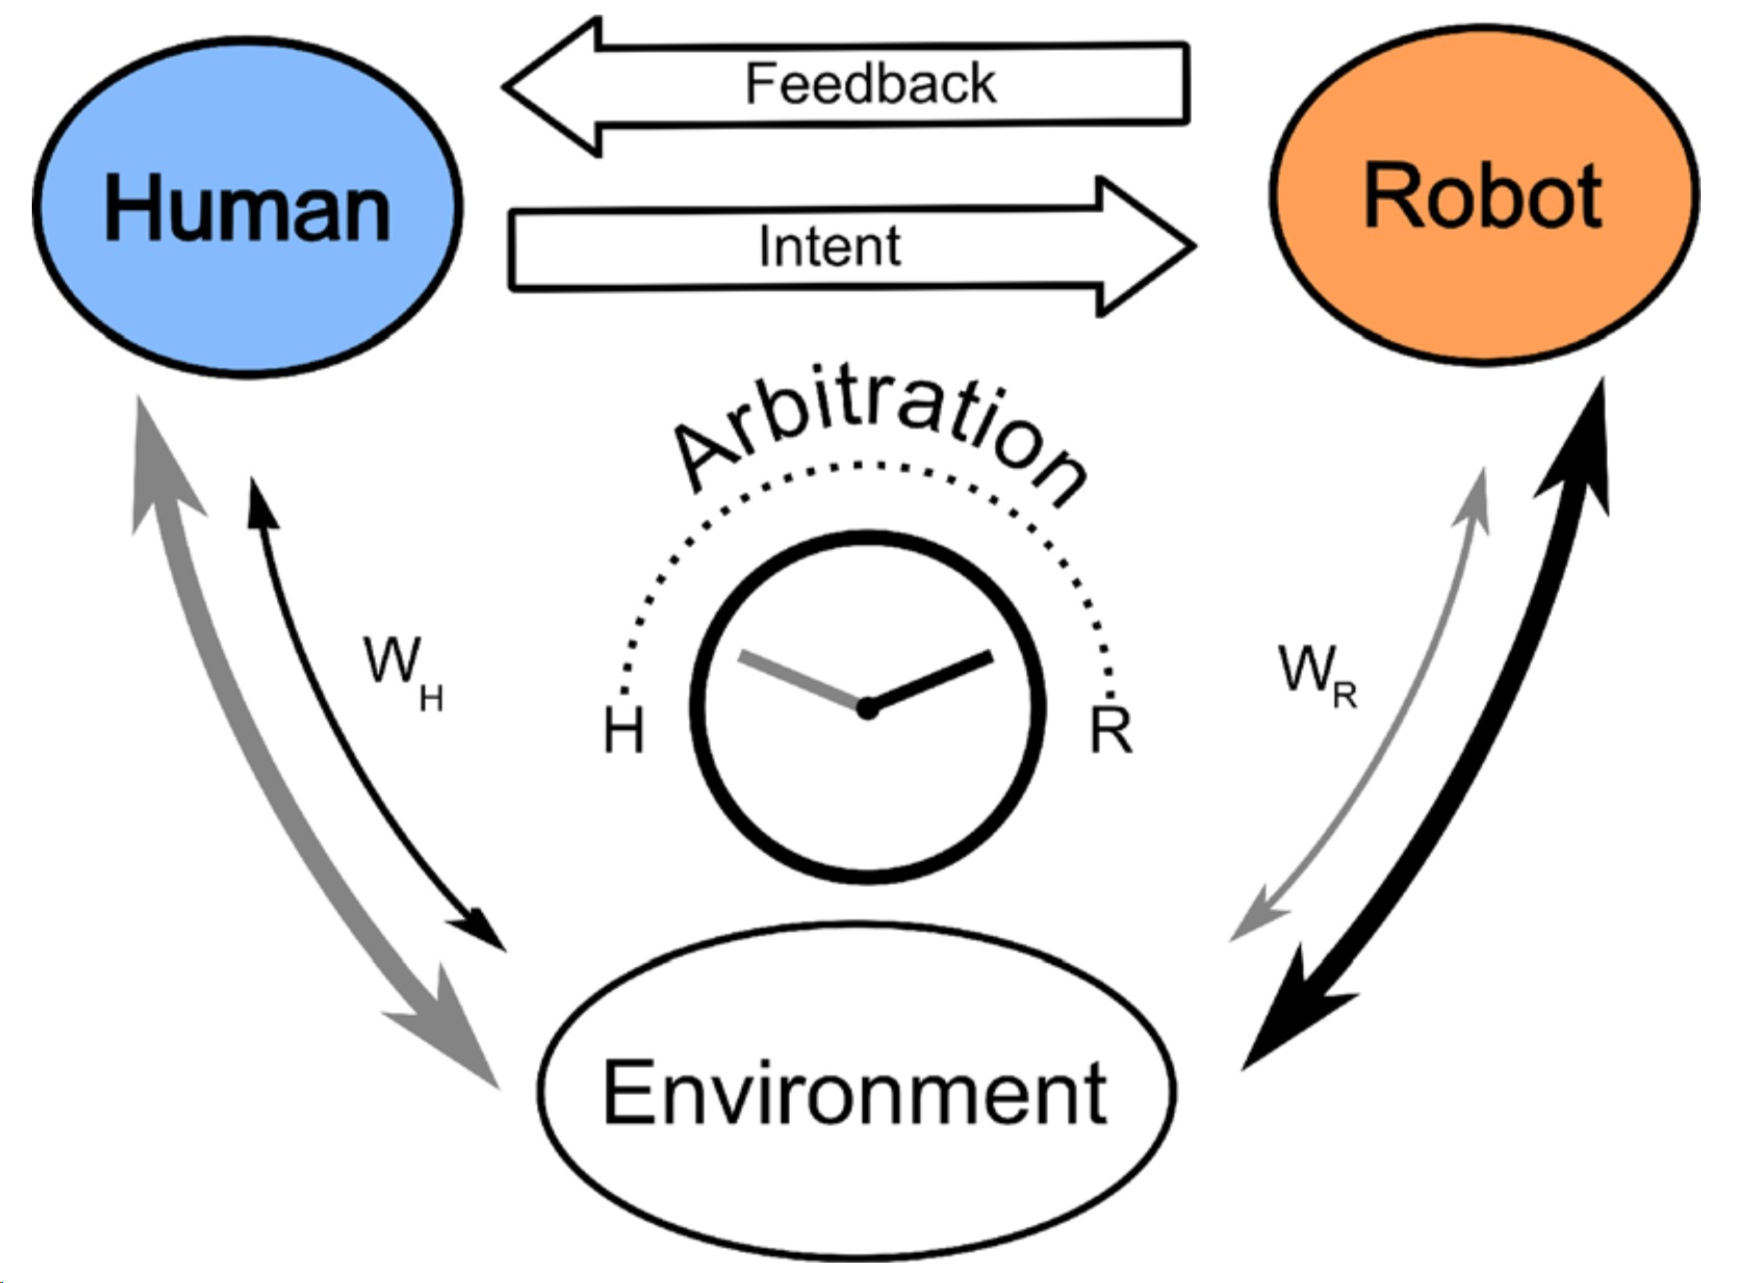
\includegraphics[width=0.8\linewidth]{figures/TradeStudy/figureb1.png}
%         \caption{Losey et al.'s proposed framework for human-robot interaction with the environment}
%         % \label{figure:}
%     \end{center}
% \end{figure}
% 	Losey et al.'s 2018 review discusses the state of the art in the field of physical human-robot interaction, where human abilities are enhanced or supported by robotic aids, and discuss the human factors involved with shared task execution between the human and robot. They present a unified view of shared human-robot control in physical task execution, using case studies of applications in healthcare to demonstrate their framework. Their framework focuses on three distinct phases of decision making: detection, the task of understanding the human's intent; arbitration, the task of distributing control between the human and robot; and feedback, the task of presenting the result of the human's intent, which is often done through haptic devices. One ongoing field of research in physical human-robot interaction is that of dynamic changes in role arbitration using machine learning and artificial intelligence techniques. The authors note role arbitration should re-evaluated when trust changes, and further note "robotic performance has the largest and most identifiable influence on trust in HRI." As such, the real-time monitoring of performance metrics is an area of active research.

% Wang, Tian-Miao, Yong Tao, and Hui Liu. "Current Researches and Future Development Trend of Intelligent Robot: A Review." International Journal of Automation and Computing (2018): 1-22.
% 	In their 2018 review, Wang et al. discuss current research and future development trends of "intelligent" robots. They note several key and leading technologies in the field of robotics. They include key technologies such as human-robot collaboration technology, autonomous navigation technology under non-structured environments, multi-agent robot systems (swarms), and emotion recognition and interaction mechanism of robot oriented to harmonious human-robot cooperation. They also highlight innovative leading technologies such as brain computer interfaces, brain-like robot control and decision making (artificial intelligence and supervised/unsupervised learning techniques), material cross-innovation and applications of robot oriented to software structure (3D printed materials, soft grippers, flexible robots), and network decision mechanism of robot based on cloud computing and big data (IoT, SLAM). Their review further breaks down these technology areas into more specific, individual technologies and notes the current state of the art in each.

\chapter{Aircraft Dynamics}

\section{Longitudinal Dynamics}
\begin{align*}
    \dot{\vec{x}}_{long} =
    \left[ \begin{array}{ *{5}{c} }
            X_u                     & X_w                     & X_q                                          & -g \cos \theta_0 & 0 \\
            Z_u                     & Z_w                     & Z_q + U_0                                    & -g \sin \theta_0 & 0 \\
            M_u + M_{\dot{w}} Z_{u} & M_w + M_{\dot{w}} Z_{w} & M_q + M_{\dot{w}} \left( Z_{q} + U_0 \right) & 0                & 0 \\
            0                       & 0                       & 1                                            & 0                & 0 \\
            0                       & -1                      & 0                                            & U_0              & 0 \\
        \end{array} \right]
    \left[ \begin{array}{ *{1}{c} }
            \Delta u      \\
            \Delta w      \\
            \Delta q      \\
            \Delta \theta \\
            \Delta z      \\
        \end{array} \right] & + \\
    \left[ \begin{array}{ *{5}{c} }
            X_{\delta_e}                            & X_{\delta_{th}}                               \\
            Z_{\delta_e}                            & Z_{\delta_{th}}                               \\
            M_{\delta_e} + M_{\dot{w}} Z_{\delta_e} & M_{\delta_{th}} + M_{\dot{w}} Z_{\delta_{th}} \\
            0                                       & 0                                             \\
            0                                       & 0                                             \\
        \end{array} \right]
    \left[ \begin{array}{ *{1}{c} }
            \Delta \delta_e    \\
            \Delta \delta_{th} \\
        \end{array} \right] &   \\
\end{align*}

\section{Lateral Dynamics}
\begin{align*}
    \dot{\vec{x}}_{lat} =
    \left[ \begin{array}{ *{5}{c} }
            Y_v  & Y_p  & Y_r - U_0     & g \cos \theta_0  & 0 \\
            L'_v & L'_p & L'_r          & -g \sin \theta_0 & 0 \\
            N'_v & N'_p & N'_r          & 0                & 0 \\
            0    & 1    & \tan \theta_0 & 0                & 0 \\
            0    & 0    & \sec \theta_0 & 0                & 0 \\
        \end{array} \right]
    \left[ \begin{array}{ *{1}{c} }
            \Delta v    \\
            \Delta p    \\
            \Delta r    \\
            \Delta \phi \\
            \Delta \psi \\
        \end{array} \right] & + \\
    \left[ \begin{array}{ *{5}{c} }
            Y_{\delta_{a}}  & Y_{\delta_{r}}  \\
            L'_{\delta_{a}} & L'_{\delta_{r}} \\
            N'_{\delta_{a}} & N'_{\delta_{r}} \\
            0               & 0               \\
            0               & 0               \\
        \end{array} \right]
    \left[ \begin{array}{ *{1}{c} }
            \Delta \delta_a \\
            \Delta \delta_r \\
        \end{array} \right] &   \\
\end{align*}



\end{document}
